\documentclass[14pt]{extreport}

\usepackage{geometry}
 \geometry{
 a4paper,
 left=30mm,
 right=15mm,
 top=20mm,
 bottom=20mm,
 }

\usepackage[utf8]{inputenc}
\usepackage[russian]{babel}
\usepackage{amsmath}
\usepackage{amssymb}
\usepackage{array}
\usepackage{tocloft}
\usepackage{etoc}
\usepackage{etoolbox}
\usepackage{indentfirst}
\usepackage{multirow}
\usepackage{ragged2e}
\usepackage{url}

\tolerance=1
\emergencystretch=\maxdimen
\hyphenpenalty=10000
\hbadness=10000

\usepackage{caption}
\usepackage{float}
\usepackage{graphicx}
\usepackage{subcaption}
\graphicspath{ {images/} }

\newcommand{\nextTitle}{String for Titles.}
\newcommand{\cursection}{0}

% These are to make TOC left-aligned.
\renewcommand{\cftchapleader}{\cftdotfill{\cftdotsep}}
\renewcommand{\cftchapfont}{\mdseries}
\renewcommand{\cftchappagefont}{\mdseries}
\cftpagenumbersoff{part}

\makeatletter
\bgroup
\advance\@flushglue by \@tocrmarg
\xdef\@tocrmarg{\the\@flushglue}%
\egroup
\makeatother
% End of left-alignment.

\begin{document}

\begin{titlepage}
    \begin{center}
        {\bf БЕЛАРУСКІ ДЗЯРЖАЎНЫ УНІВЕРСІТЭТ}
    \end{center}
    \begin{center}
        {\bf Факультэт прыкладной матэматыкі і інфарматыкі}
    \end{center}
    \begin{center}
        Кафедра дыскрэтнай матэматыкі і алгарытмікі
    \end{center}

    \vspace{8em}

    \begin{center}
        \textbf{
          Справаздача \\
          аб праходжанні пераддыпломнай практыкі
        }
    \end{center}

    \vspace{3em}

    \begin{flushright}
        студэнта 4 курса \\
        Богдана Уладзіслава Уладзіміравіча \\
        спецыяльнасць ``інфарматыка'' \\
    \end{flushright}

    \vspace{1em}

    \begin{flushright}
        Кіраўнік практыкі:\\
        асістэнт Жылка Андрэй Ігаравіч \\
    \end{flushright}

    \vfill

    \begin{center}
        Мінск, 2018
    \end{center}
\end{titlepage}
\newpage


\begin{titlepage}
    \begin{center}
        \section*{РЭФЕРАТ}
    \end{center}

    \vspace{10mm}

    Дыпломная праца, 41 с., 16 выяў, 5 формул, 18 крыніц

    \vspace{4mm}

    БПЛА, ТРОХМЕРНАЯ РЭКАНСТРУКЦЫЯ, СТЭРЭАБАЧАННЕ, SLAM-АЛГАРЫТМЫ,
    ЭПІПАЛЯРНАЯ ГЕАМЕТРЫЯ, МАНАКУЛЯРНАЯ КАМЕРА, КЛЮЧАВЫЯ КРОПКІ,
    ДЭСКРЫПТАРЫ КЛЮЧАВЫХ КРОПАК, ПОШУК АДПАВЕДНАСЦЯЎ

    \vspace{4mm}

    Аб'ектам даследвання з'яўляюцца алгарытмы трохмернай рэканструкцыі паверхні
    па дадзеных з беспілотных лятальных апаратаў.

    \vspace{4mm}

    Мэта працы –- даследаваць будову алгарытмаў рэканструкцыі паверхні па наборы здымкаў,
    правесці аналіз існуючых SLAM-алгарытмаў, разгледзець магчымасці інтэграцыі двух падыходаў
    да рэканструкцыі паверхні, расправаць адпаведнае праграмнае забеспячэнне.

    \vspace{4mm}

    Метады даследвання: аналіз публікацыяў і вынікаў эксперыментаў,
    даследванне ўнутранай будовы алгарытмаў,
    правядзенне уласных эксперыментаў, распрацоўка праграмнага забеспячэння.

    \vspace{4mm}

    У ходзе працы атрыманыя наступныя вынікі:

    \vspace{4mm}

    \begin{enumerate}
        \item Праведзены аналіз і прыведзеная апісанне сучасных SLAM-алгарытмаў.
        \item Прапанаваныя падыходы, пры якіх SLAM-алгарытмы могуць быць інтэграваныя з
        класічнымі алгарытмамі для рэканструкцыі паверхні па дадзеных з беспілотных лятальных апаратаў.
        \item Распрацаванае праграмнае забеспячэнне для маніпуляцыі з наборамі дадзеных,
        пабудовы трохмерных мадэляў па наборы здымкаў, візуалізацыі. Праграмнае забеспячэнне,
        апроч рэалізацыі традыцыйных падыходаў да рэканструкцыі, інтэграванае з SLAM-сістэмамі,
        адкуль яно вымае дадатковыя дадзеныя і выкарыстоўвае для ўдасканалення сваёй працы.
    \end{enumerate}

    \vspace{4mm}

    Галіны прымянення: камп'ютарны зрок, трохмерная рэканструкцыя, іншыя прыкладанні.
\end{titlepage}

\newpage

\begin{titlepage}
    \begin{center}
        \section*{РЕФЕРАТ}
    \end{center}

    \vspace{10mm}

    Дипломная работа, 40 с., 16 изображений, 5 формул, 18 источников

    \vspace{4mm}

    БПЛА, ТРЁХМЕРНАЯ РЕКОНСТРУКЦИЯ, СТЕРЕОМЕТРИЯ, SLAM-АЛГОРИТМЫ, ЭПИПОЛЯРНАЯ ГЕОМЕТРИЯ,
    МОНОКУЛЯРНАЯ КАМЕРА, КЛЮЧЕВЫЕ ТОЧКИ, ДЕСКРИПТОРЫ КЛЮЧЕВЫХ ТОЧЕК, ПОИСК СООТВЕТСТВИЙ

    \vspace{4mm}

    Объектом исследования являются алгоритмы трёхмерной реконструкции поверхности
    по данным с беспилотных летательных аппаратов.

    \vspace{4mm}

    Цель работы –- исследовать строение алгоритмов реконструкции поверхности по набору снимков,
    провести анализ существующих SLAM-алгоритмов, рассмотреть возможности интеграции двух подходов
    к реконструкции поверхности, разработать соответствующее программное обеспечение.

    \vspace{4mm}

    Методы исследования: анализ публикаций и результатов экспериментов,
    исследование внутреннего строения алгоритмов, проведение собственных экспериментов,
    разработка программного обеспечения.

    \vspace{4mm}

    В ходе работы получены следующие результаты:

    \vspace{4mm}

    \begin{enumerate}
        \item Проведён анализ и приведено описание современных SLAM-алгоритмов.
        \item Предложены подходы, при которых SLAM-алгоритмы могут быть интегрированы с классическими
        алгоритмами для реконструкции поверхности по данным с беспилотных летательных аппаратов.
        \item Разработано программное обеспечение для манипуляции с наборами данных,
        построения трёхмерных моделей па набору снимков, визуализации.
        Программное обеспечение, кроме реализации традиционных подходов к реконструкции,
        интегрировано с SLAM-системами, откуда оно достаёт дополнительные данные и использует для своей работы.
    \end{enumerate}

    \vspace{4mm}

    Область применения: компьютерное зрение, трёхмерная реконструкция, приложения.
\end{titlepage}

\newpage

\begin{titlepage}
    \begin{center}
        \section*{ABSTRACT}
    \end{center}

    \vspace{10mm}

    Graduate work, 41 p., 16 figures, 5 formulas, 18 sources

    \vspace{4mm}

    UAV, THREE-DIMENSIONAL RECONSTRUCTION, STEREOVISION, SLAM ALGORITHMS,
    EPIPOLAR GEOMETRY, MONOCULAR CAMERA, KEYPOINTS, FEATURES, FEATURES’ DESCRIPTORS,
    FEATURE MATCHING

    \vspace{4mm}

    The object of the research are algorithms of three-dimensional reconstruction
    of the surface based on the data from unmanned aerial vehicles.

    \vspace{4mm}

    The purpose –- to research the structure of the algorithms of surface reconstruction
    from a set of images, to analyze existing SLAM algorithms,
    to search for the possibilities to integrate two reconstruction approaches, to develop the software.

    \vspace{4mm}

    Methods of the research are: to analyze publications and results of the experiments,
    to research internal structure of the algorithms, to perform own experiments, to develop the software.

    \vspace{4mm}

    During the research the following results were obtained:

    \vspace{4mm}

    \begin{enumerate}
        \item Analysis of state-of-art SLAM algorithms was performed and the description was provided.
        \item The ways to integrate SLAM algorithms with traditional algorithms
        for surface reconstruction based on the data from UAV were suggested.
        \item The software for data manipulation, three-dimensional models’
        construction and visualization was developed. Furthermore, the software was
        integrated with SLAM systems in order to obtain data to improve its work.
    \end{enumerate}

    \vspace{4mm}

    The scopes are: computer vision, three-dimensional reconstruction, other applications.
\end{titlepage}

\newpage


\setcounter{page}{2}
\renewcommand*\contentsname{Змест}

\tableofcontents

\newpage

\begin{center}
    \addcontentsline{toc}{section}{УВОДЗІНЫ}
    \section*{УВОДЗІНЫ}
\end{center}

Задача рэканструкцыі паверхні зямлі па дадзеных з беспілотных лятальных апаратаў
(БПЛА) узнікае ўсё ў большай колькасці сфераў жыцця: ад сельскай гаспадаркі да
ацэнкі наступстваў прыродных катастрофаў. Патрэбнасць у эфектыўным рашэнні
задачы таксама звязаная з шырокай даступнасцю БПЛА і камер.

Непасрэдна задача рэканструкцыі цесна звязаная са шматлікімі сумежнымі задачамі:
распазнаванне аб'ектаў, навігацыя ў прасторы, пабудова мапы мясцовасці.
Асаблівую цікаўнасць прадстаўляюць рашэнні, якія выконваюцца ў рэальным часе;
праца ў рэальным часе для алгарытмаў навігацыі і абхода перашкодаў можа быць крытычнай для
аўтаномных БПЛА, у адрозненні ад наземных робатаў, якія могуць на нейкі час спыніцца і
дачакацца пабудовы маршрута.

У гэтай працы я падсумую найважнейшыя аспекты, якія ўзнікаюць пры рашэнні задачы
рэканструкцыі паверхні, а таксама разгледжу шэраг алгарытмаў з агульнай назвай
SLAM (Simultaneous Localization and Mapping), якія могуць быць эфектыўна прымененыя
да задачаў, якія патрабуюць найбольшай хуткасці выканання, такіх як навігацыя.

\newpage


\begin{center}
    \renewcommand{\nextTitle}{ГЛАВА 1. АКТУАЛЬНАСЦЬ ЗАДАЧЫ РЭКАНСТРУКЦЫІ ПАВЕРХНІ}
    \addcontentsline{toc}{section}{\nextTitle}
    \section*{\nextTitle}
\end{center}

\vspace{5mm}

\renewcommand{\cursection}{1}
\setcounter{figure}{0}

\renewcommand{\nextTitle}{1.1 Агульныя звесткі}
\addcontentsline{toc}{subsection}{\nextTitle}
\subsection*{\nextTitle}

У агульным выпадку задача рэканструкцыі паверхні фармулюецца наступным чынам:
неабходна рэканструяваць трохмерны аб'ект па мностве зробленых з розных ракурсаў
здымкаў. Задача фармулюецца дастаткова натуральна чынам, і калі чалавеку дастаткова кінуць
позірк на аб'ект, каб уявіць ягоную трохмерную структуру, алгарытмічна задача
ўсё яшчэ застаецца не да канца вырашанай, звычайна патрабуе вялікіх вылічальных магутнасцяў
і не працуе ўніверсальна добра для любых асяроддзяў і любых умоваў здымак, такіх як,
напрыклад, адрозныя па асвятленні сцэны.
Пад трохмерным аб'ектам у залежнасці ад кантэксту могуць мецца на ўвазе адрозныя рэчы:
калі ў некаторых сітуацыях раздрэджанае воблака кропак будзе лічыцца добрым прыкладам
рэканструяванай структуры, то ў іншых пастаўленая задача можа запатрабаваць пабудову
шчыльнай і гладкай мадэлі з нанесенымі тэкстурамі і колерамі. Падбор алгарытмаў і
ацэнка вылічальных магутнасцяў здзяйсняецца ў залежнасці ад пастаўленых патрабаванняў.

Задача рэканструкцыі можа таксама фармулявацца для іншых тыпаў уваходных дадзеных:
апроч той ці іншай камеры ўваходнымі дадзенымі для задачы могуць быць
дадзеныя з іншых датчыкаў, такіх як акселерометр, гіраскоп ці GPS-датчык;
замест манакулярнай камеры можа прымяняцца RGB-D камера (вяртае дадатковы слой глыбіняў)
стэрэа-камера (уяўляе сабой дзве RGB камеры на фіксаванай паміж сабой адлегласці,
якія ў пэўным сэнсе імітуюць бінакулярны чалавечы зрок), альбо, напрыклад, лазерная камера.

Варта дадаць, што даследаванні ў гэтай галіне камп'ютарнага зроку развіваюцца
таксама праз удасканаленне апаратнага забеспячэння: падыходы, якія некалькі год
таму былі практычна нерэалізуемымі і былі магчымыя толькі ў тэорыі,
з развіццём тэхналогіяў атрымліваюць новае жыццё.

Разам з тым, мноства праблемаў застаюцца нявырашанымі. Поспех усёй галіны даследаванняў
залежыць ад таго, наколькі адначасова добра будуць удасканальвацца вылічальныя магутнасці
камп'ютарных сістэм, алгарытмы, а таксама сродкі захопу дадзеных - усё яшчэ мноства праблем
узнікае акурат праз недасканаласць, недакладнасць альбо нестабільнасць камер і іншых датчыкаў.

\renewcommand{\nextTitle}{1.2 Сферы прымянення}
\addcontentsline{toc}{subsection}{\nextTitle}
\subsection*{\nextTitle}

Цікавасць задачы рэканструкцыі таксама ў запатрабаванні атрымання рашэння ў абсалютна розных сферах
жыцця, кожная з якіх дыктуе свае асаблівасці і прымушае развіваць даследаванні ў тым ці іншым кірунку.

БПЛА выкарыстоўваюцца надзвычайнымі службамі для ацэнкі наступстваў прыродных катастроф,
у сельскай гаспадарцы, дарожнымі службамі для маніторынгу і аналізу трафіка.
Патрабаванні да хуткасці працы алгарытмаў рэканструкцыі
натуральныя - хуткасць працы ў некаторых галінах жыцця крытычная і разбор вялікіх аб'ёмаў
неапрацаваных дадзеных можа стацца непераадольна вялікай працай для чалавека. Патрабаванне да алгарытмаў
рэканструкцыі працаваць у рэальным часе ў большасці выпадкаў з'яўляецца пры навігацыі і
аўтаномным руху, у такім выпадку шчыльная рэканструкцыя можа быць залішняй і
разрэджаная мадэль у выглядзе воблака кропак цалкам задаволіць патрабаванні. У такіх выпадках
мы часта кажам пра пабудову мапы - аб'екта, які ўяўляе сабой своеасаблівую мадэль навакольнага
свету, з пазначанымі на ім кропкамі, якія прадстаўляюць для нас цікаўнасць. Мапы часта
выкарыстоўваюцца для лакалізацыі і навігацыі і могуць быць схаваныя ад вачэй назіральніка.
Падрабязней да тэмы пабудовы мапаў мы вернемся падчас абмеркавання SLAM-алгарытмаў.

\renewcommand{\nextTitle}{1.3 Асаблівасці задачы пры выкарыстанні БПЛА}
\addcontentsline{toc}{subsection}{\nextTitle}
\subsection*{\nextTitle}

Той факт, што рэканструкцыя адбываецца не на выпадковым наборы дадзеных, пра які адсутнічае дадатковая інфармацыя,
дае нам прастору для аптымізацыі працэса рэканструкцыі: скарачэнне часу і паляпшэнне якасці пабудаванай мадэлі.
Пералічым асаблівасці задачы рэканструкцыі па дадзеных з БПЛА ў параўнанні з агульнай задачай:
\begin{itemize}
    \item Усе здымкі зробленыя адной фізічнай камерай, такім чынам унутраныя параметры ўсіх камераў застаюцца нязменнымі.
    Больш за тое, унутраныя параметры камеры застаюцца нязменнымі не толькі ў межах аднаго набора,
    але і для ўсіх здымкаў зробленым адным БПЛА з зафіксаванай на ім камерай.
    Апошні факт не ўносіць зменаў у працэс рэканструкцыі, але спрашчае працэс выкарыстання БПЛА на практыцы
    (адсутнасць патрэбы ў шторазовым калібраванні для высвятлення ўнутраных параметраў камеры).
    \item Апроч камеры ў нашым распараджэнні, у залежнасці ад канфігурацыі БПЛА, могуць мецца і іншыя датчыкі:
    акселерометр, гіраскоп, GPS-датчык і інш.
    Дадзеныя сабраныя імі, могуць выкарыстоўвацца як для вызначэння вонкавых параметраў камеры,
    так і для папярэдняга размяшчэння кропак у прасторы.
\end{itemize}

\subsubsection*{Патэнцыйныя змены ў набор дадзеных і алгарытмы з улікам вышэйсказанага}

Прычыны, па якіх дадатковыя дадзеныя станоўча паўплываюць на якасць і хуткасць рэканструкцыі, абсалютна натуральныя:
памяншэнне колькасці параметраў у глабальнай аптымізацыйнай задачы і больш якасная пачатковая апраксімацыя.
Такім чынам мы маем два падыходы да выкарыстання дадзеных, якімі суправаджаецца набор выяваў:
\begin{itemize}
    \item Аб'яўленне параметраў канстантнымі і непасрэдная іх падстаноўка ва ўраўненні - такім чынам,
    маем яўнае памяншэнне колькасці параметраў што не можа не паўплываць на хуткасць адпрацоўкі алгарытма
    і на выніковае значэнне памылкі праекцыі станоўча.
    Відавочны і недахоп: немагчымасць дакладнага папярэдняга задання параметраў і наступнае аб'яўленне іх канстантнымі
    прывядзе да псавання канчатковых значэнняў трохмерных кропак і, адпаведна, пагаршэння якасці пабудаванай мадэлі.
    Дакладнасць вызначэння параметраў знаходзіцца ў простай залежнасці ад карэктнасці пабудаванай мадэлі.
    На практыцы высвятляецца, што такі падыход вядзе да значнага пагаршэння канчатковых вынікаў
    і кепска прымяняльны на рэальных дадзеных.
    \item Выкарыстанне дадатковых дадзеных для пачатковай апраксімацыі значэнняў параметраў камеры і
    палажэнняў кропак у прасторы. Пры такім падыходзе, мы не рызыкуем стаць ахвярамі кепскай дакладнасці
    альбо памылак у апісанні дадзеных - разам з тым, колькасць ітэрацый у працэсе пучковай аптымізацыі
    можа паменшыцца ў разы. Гэты падыход можа паспяхова быць прыменены на практыцы:
    хуткасць працэса пабудовы проста залежыць ад якасці ўваходных дадзеных -
    яўных жа памылак у выніковай мадэлі (такіх, як у першым пункце) назірацца не будзе,
    бо алгарытм выправіць яўна хібныя ўваходныя дадзеныя.
\end{itemize}

Альтэрнатывай можа стаць змяшаны падыход: напрыклад, аб'явіць фокусную адлегласць пастаяннай
і недаступнай да зменаў (калі мы дастаткова ўпэўненыя ў лічбах, якія прадастаўляе вытворца камера,
альбо атрыманых у выніку каліброўцы), але дазволіць алгарытму удакладняць параметры павароту камеры -
пры дастаткова дакладных пачатковых значэннях яны будуць змененыя нязначна.

Апісаныя вышэй падыходы я выкарыстоўваю ў сваім распрацаваным праграмным забеспячэнні,
падрабязнае апісанне якога прыводзіцца ў апошняй главе.

\newpage

\begin{center}
    \renewcommand{\nextTitle}{ГЛАВА 2. ТЭАРЭТЫЧНЫЯ АСПЕКТЫ ЗАДАЧЫ РЭКАНСТРУКЦЫІ}
    \addcontentsline{toc}{section}{\nextTitle}
    \section*{\nextTitle}
\end{center}

\vspace{5mm}

\renewcommand{\cursection}{2}
\setcounter{figure}{0}

\renewcommand{\nextTitle}{2.1 Этапы рашэння задачы рэканструкцыі}
\addcontentsline{toc}{subsection}{\nextTitle}
\subsection*{\nextTitle}

\vspace{5mm}

Калі мы вядзем гаворку пра пабудову трохмернай мадэлі па здымках з адзінай
манакулярнай камеры, мы заўсёды рашаем некалькі важных задач. Да гэтых задач
адносяцца:
\begin{itemize}
    \item для двух ці некалькі кадраў -- выманне інфармацыі аб агульнай аглядаемасці сцэны;
    \item для здымка (пры наяўнасці іншых дадзеных) - пабудова мапы глыбіні сцэны;
    \item рашэнне аптымізацыйнай задачы па аб'яднанні ўсёй інфармацыі
    ў адзіную сцэну (ці прыняцце рашэння аб наяўнасці некалькіх незалежных
    сцэн у межах аднаго набора дадзеных), мінімізацыя геаметрычных і аптычных памылак.
\end{itemize}

Гэтыя задачы ў той ці іншай форме і ў тым ці іншым выглядзе з'яўляюцца пры любой
спробе рэканструяваць трохмерную паверхню сродкамі камп'ютарнага зроку.
Спынімся на першай задачы і паглядзім падрабязней, якія наборы інструментаў даюць магчымасць
ацаніць узаемаразмяшчэнне для двух ці некалькіх здымкаў і, такім чынам, даць уяўлянне
пра арганізацыю камераў вакол сцэны.

Першы з такіх набораў інструментаў -- метады,
заснаваныя на \textit{пошуку асаблівасцяў} (англ. \textit{feature-based methods}).
Ідэя у выманні з кожнай асобнай выявы пэўнай колькасці асаблівасцяў (імі могуць быць,
напрыклад, кропкі, вуглы альбо лініі) і пошук адпаведнасцяў паміж асаблівымі кропкамі
на розных выявах (англ. \textit{feature matching}),
аднаўленне пазіцыяў камер і структуры сцэны з дапамогай эпіпалярнай геаметрыі (геаметрыя стэрэабачання) і,
у завяршэнне, удакладненне параметраў праз мінімізацыю памылкі праекцыі. Падобную працэдуру выконвае
вялікая колькасць алгарытмаў: даступнасць эфектыўных метадаў вымання асаблівасцяў і пошуку іх адпаведнасцяў
дазваляе рабіць гэта хутка і надзейна; разам з тым, такі падыход можа даваць недастатковую дакладнасць вынікаў,
быць прымяняльным толькі на вызначаным класе зыходных дадзеных (напрыклад, не дапускаць аднастайныя тэкстуры),
патрабуе надзейных алгарытмаў ацэнкі пазіцыі.

Другі клас метадаў заснаваны на гэтак званых \textit{простых метадах}
(англ. \textit{direct methods}): у такіх метадах непасрэдна выкарыстоўваюцца значэнні
запісаныя ў пікселях, не адбываецца спробы выяўлення на выяве вызначанага
кшталту асаблівасцяў. Для апрацоўкі выкарыстоўваецца накірунак і велічыні
лакальнага градыента інтэнсіўнасці. Простыя метады, якія выкарыстоўваюць усю
інфармацыю на выяве, нават у зонах з маленькім градыентам, апынуліся значна
эфектыўнейшымі за метады, заснаваныя на пошуку асаблівасцяў у сцэнах з нізкай
тэкстураванасцю альбо ў выпадку размытасці ці дэфакусіроўкі \cite{direct-methods}.
Дастаткова працазатратнай працэдурай становіцца падлік фотаметрычнай памылкі
(у параўнанні з падлікам памылкі праекцыі).
Разам з тым, паколькі праца вядзецца непасрэдна са значэннямі пікселяў,
час эканоміцца на пошуку асаблівасцяў і падліку дэскрыптараў.

\renewcommand{\nextTitle}{2.2 Тыпы камер}
\addcontentsline{toc}{subsection}{\nextTitle}
\subsection*{\nextTitle}

Неглядзячы на цікавыя магчымасці такіх датчыкаў, як акселерометр, гіраскоп альбо
лазер вымярэння адлегласці, яны не заўсёды даступныя і не даюць універсальна добрых
вынікаў у любых умовах. Далей мы будзем весці гутарку пра камеры розных тыпаў і
больш за ўсё - пра манакулярную, як найбольш універсальную, распаўсюджаную і простую
ў эксплуатацыі.

\renewcommand{\nextTitle}{2.2.1 Стэрэа RGB камера}
\addcontentsline{toc}{subsubsection}{\nextTitle}
\subsubsection*{\nextTitle}

Для стэрэакамеры ўласцівая наяўнасць двух ці больш аб'ектываў, кожны з якіх
стварае кадры незалежна ад іншага. Гэта дазваляе сімуляваць бінакулярны зрок чалавека
і атрымліваць трохмерныя аб'екты са значна меншымі вылічальнымі выдаткамі.
Кожны з аб'ектываў стэрэакамеры працуе як асобная манакулярная камера, плыні кадраў
з розных аб'ктываў даюць магчымасць праз пошук асаблівых кропак і геаметрычныя падлікі
размясціць кропкі ў трохмернай прасторы.

Трэба дадаць, што стэрэакамера заўжды наладжаная на працу з пэўным спектрам адлегласцяў:
камера, якая працуе добра ў маленькіх закрытых прасторах не дасць такіх жа вынікаў,
калі прастора будзе змасштабаваная ў дзясяткі разоў. Такім чынам, стэрэакамерам не
ўласцівая вялікая універсальнасць.

\renewcommand{\nextTitle}{2.2.2 RGB-D камера}
\addcontentsline{toc}{subsubsection}{\nextTitle}
\subsubsection*{\nextTitle}

RGB-D камера, як і стэрэа, з'яўляецца шматканальнай: разам з RGB каналам, які
вяртае звыклыя нашаму воку каляровыя выявы, існуе дадатковы канал, які для кожнага
здымка вяртае гэтак званую мапу глыбіняў. Прыклад вяртаемых дадзеных - на малюнку
\cursection.\ref{fig:rgbd-example}.

На практыцы RGB-D камеры не заўсёды працуюць так добра, як нам хацелася б:
справа ў абмежаванасці спектра, у якім фармуюцца значэнні глыбіняў. Мапа глыбіняў,
атрыманая апаратным спосабам, часцей за ўсё выкарыстоўваецца для папярэдняй ініцыялізацыі
і для паслядоўнай аптымізацыі алгарытмічнымі спосабамі. Да таго ж, RGB-D камеры
даюць слабыя вынікі ў складаных умовах, такіх як уздзеянне простых сонечных прамянёў.

Прыкладамі RGB-D камер з'яўляюцца Kinect для Xbox 360 альбо Intel RealSense камеры.

\begin{figure}[H]
\centering
\begin{subfigure}{.5\textwidth}
  \centering
  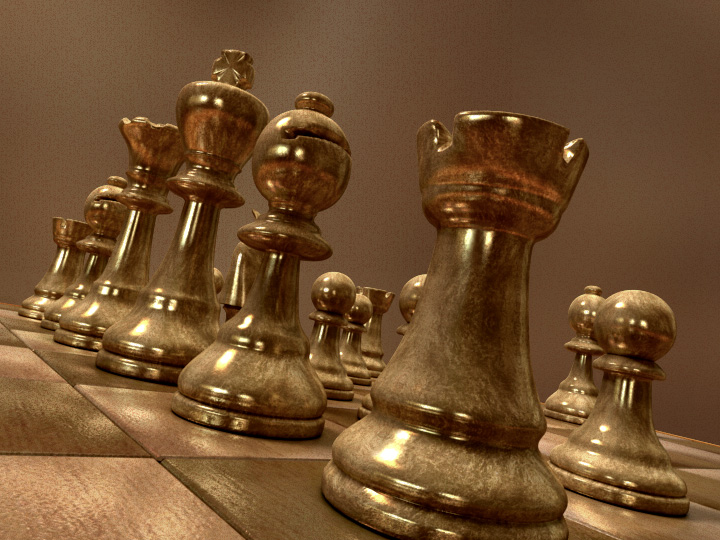
\includegraphics[width=.95\linewidth]{chess_rgb.jpg}
\end{subfigure}%
\begin{subfigure}{.5\textwidth}
  \centering
  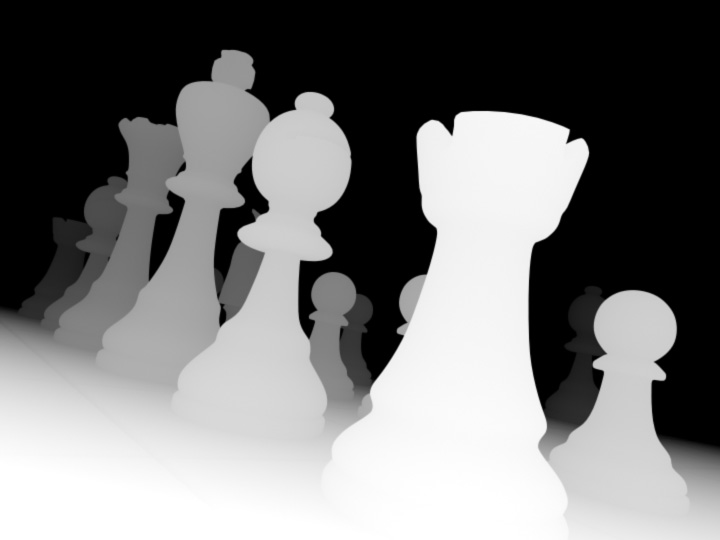
\includegraphics[width=.95\linewidth]{chess_d.jpg}
\end{subfigure}
\captionsetup{labelformat=empty}
\caption{Малюнак \cursection.\arabic{figure}: здымкі з RGB-D камеры}
\label{fig:rgbd-example}
\end{figure}

\renewcommand{\nextTitle}{2.2.3 Манакулярная RGB камера}
\addcontentsline{toc}{subsubsection}{\nextTitle}
\subsubsection*{\nextTitle}

Самымі распаўсюджанымі з'яўляюцца добра знаёмыя нам манакулярныя камеры - камеры, якія прысутнічаюць
у смартфонах і ўжываюцца ў быце.
Манакулярныя камеры, ў сваю чаргу, таксама бываюць розных тыпаў,
але на практыцы мы часцей за ўсё працуем з праектыўнымі (англ. ``projective'', ``pinhole'') камерамі.

Да таго ж гэта адзіны від камераў, з якімі ў рамках дадзенай работы вялася шчыльная праца,
для якіх рэалізаваныя алгарытмы і на якіх праводзіліся эксперыменты.

Праецыраванне трохмерных кропак у выпадку з манакулярнай камерай можа быць апісанае наступнай формулай:

\begin{equation}
  x = PX
\end{equation}

\vspace{4mm}

дзе $P$ - матрыца, якая здзяйсняе пераўтварэнне, $X, x$ - вектары, якія адпавядаюць
трохмернай і двухмернай кропцы адпаведна, запісаныя ў аднародных каардынатах.
У сваю чаргу матрыцу $P$ можна прадставіць як:

\begin{equation} \label{eq:transform-matrix}
  P = K[R|t]
\end{equation}

\vspace{4mm}

дзе $K$ - вектар унутраных параметраў камеры, $R$ - $3 \times 3$ матрыца павароту, $t$ - $3 \times 1$ вектар
зрушэння камеры ў прасторы ў сусветных каардынатах. Гэтыя параметры задаюць праектыўную
камеру, якая здзяйсняе праекцыю кропкі прасторы на матрыцу камеры. Унутраныя параметры могуць
задавацца разнастайным чынам, распаўсюджанымі прыкладамі выступаюць матрыцы:

\begin{equation}
  K = \begin{bmatrix}
    f & 0 & p_x \\[0.3em]
    0 & f & p_y \\[0.3em]
    0 & 0 & 1
  \end{bmatrix},
  \hspace{5mm}
  K = \begin{bmatrix}
    \alpha_x & 0 & p_x \\[0.3em]
    0 & \alpha_y & p_y \\[0.3em]
    0 & 0 & 1
  \end{bmatrix}
\end{equation}

\vspace{4mm}

дзе $f$ - фокусная адлегласць, $\alpha_x$, $\alpha_y$ - фокусная адлегласць уздоўж восяў
(для выпадкаў, калі не супадае), $p_x$, $p_y$ - зрушэнні цэнтру праекцыі адносна цэнтра матрыцы.
Іншымі параметрамі камеры могуць быць радыяльныя скажэнні $k_1, k_2$, якія ўзнікаюць з-за неідэальнасці
лінзаў у камерах.

\begin{figure}[h]
    \centering
    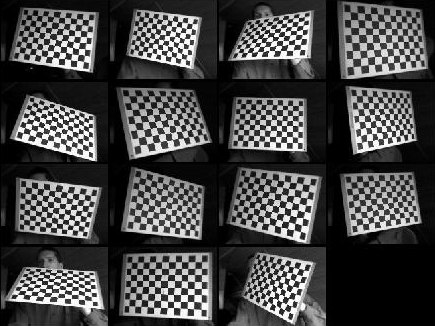
\includegraphics[width=0.8\textwidth]{calibration.jpg}
    \captionsetup{labelformat=empty}
    \caption{Малюнак \cursection.\arabic{figure}: працэс каліброўкі манакулярнай камеры}
    \label{fig:calibration}
\end{figure}

Унутраныя параметры камеры заўжды вядомыя загадзя альбо праз дакументацыю да прылады ад
вытворца, альбо праз каліброўку: каліброўка можа выяўляць хібы, дапушчаныя вытворцам.
Каліброўка дае добрыя значэнні ўнутраных параметраў
камеры, таму яны рэдка выкарыстоўваюцца ў якасці аптымізуемых параметраў.
Працэс каліброўкі, у выпадку патрэбы, не складана здзейсніць самастойна - існуе вялікая колькасць утылітаў
(напрыклад, у складзе OpenCV), якія дазваляюць гэта зрабіць, маючы ў наяўнасці толькі раздукаваную
дошку, якая нагадвае шахматную, памерамі 9x7 клетак (гэты параметр вар'юецца).
Працэс каліброўкі паказаны на малюнку \cursection.\ref{fig:calibration}.

У сваю чаргу, матрыца $R$ і вектар $t$ ва ўраўненні \ref{eq:transform-matrix} з'яўляюцца
\textit{знешнімі параметрамі камеры} і вызначаюцца пазіцыяй камеры ў прасторы.

Варта зазначыць, што адной з найбольшых перавагаў і, адначасова, адной з найбольшых
перашкодаў у працы ў манакулярнымі камерамі з'яўляецца неадназначнасць працы з масштабам.
Праблема ў тым, што масштаб не можа быць высветлены праз перасоўванні ў прасторы і
змяненні ў вуглах агляду, што з'яўляецца крыніцай мноства памылак. Разам з тым,
перавага неадназначнасці масштабу ва ўніверсальнасці: алгарытм будзе працаваць
з аднолькавымі вынікамі як у маленькіх закрытых памяшканнях, так і на вялікіх
адкрытых прасторах. З гэтым аспектам (немачыгмасць высвятлення рэальных памераў аб'ектаў)
мы яшчэ сутыкнемся пры абмеркаванні SLAM-алгарытмаў - некаторыя з іх, такія як
CNN-SLAM (\cite{DBLP:journals/corr/TatenoTLN17}), прапаноўваюць шляхі вырашэння гэтай праблемы.

\subsubsection*{Заданне матрыцы павароту праз кватэрніоны}

\vspace{5mm}

Альтэрнатывай апісанай вышэй матрыцы павароту памера $3 \times 3$
можа быць апісанне павароту з дапамогай кватэрніонаў.

{\bf Кватэрніоны} - сістэма гіперкамплексных лікаў,
якія ўтвараюць вектарную прастору размернасцю 4 над полем рэчаісных лікаў.

Кватэрніон можа быць прадстаўлены як фармальная сума
$q(a, b, c, d) = a + bi + cj + dk$, дзе $a, b, c, d \in\mathbb{R}$, $i, j, k$ -
уяўныя адзінкі, такія, што $i^2 = j^2 = k^2 = ijk = -1$.

Кватэрніон часта запісываецца як пара $(a, \vec{u})$, дзе $a \in\mathbb{R}$,
$\vec{u} = (b, c, d) \in\mathbb{R}^3$ - вектар у трохмернай прасторы,
што дае нагоду задумацца аб прымяненні кватэрніонаў для заданняў паваротаў у трохмернай прасторы.

Негледзячы на тое, што агулам кватэрніоны не знайшлі шырокага прымянення,
іх выкарыстанне часта апраўданае ў некаторых галінах матэматыкі ды інфарматыкі,
такіх як камп'ютарная графіка, навігацыя альбо праграмаванне гульняў.
Кватэрніоны мінімальнай колькасцю скалярных параметраў задаюць паварот,
пры гэтым яны пазбаўленыя выраджанасці, якая сустракаецца пра заданні паварота
пры дапамозе толькі трох параметраў (напрыклад - вугламі Эйлера).

Калі маем кватэрніон $q = (w, x, y, z)$, тады матрыца павароту можа быць запісаная праз кватэрніон як:
\begin{equation} \label{eq:quaternion-to-rotation}
    R = \left( \begin{array}{ccc}
    1 - 2y^2 - 2z^2 & 2xy - 2zw & 2xz + 2yw \\
    2xy + 2zw & 1 - 2x^2 - 2z^2 & 2yz - 2xw \\
    2xz - 2yw & 2yz + 2xw & 1 - 2x^2 - 2y^2 \end{array} \right)
\end{equation}

У практычнай рэалізацыі з главы 4 кватэрніоны выкарыстоўваюцца пры перадачы знешніх
параметраў камер паміж кампанентамі сістэмы,
схематычна прадстаўленай на малюнку 4.\ref{fig:architecture}.

\renewcommand{\nextTitle}{2.3 Ключавыя кропкі, дэскрыптары, спосабы іх апісання}
\addcontentsline{toc}{subsection}{\nextTitle}
\subsection*{\nextTitle}

\vspace{5mm}

Тут і далей мы будзем казаць пра ``ключавыя кропкі'' (англ. \textit{keypoints})
альбо ``асаблівасці'' (англ. \textit{features}), хаця ў тэрмінах таго ці іншага дэтэктара
ключавой кропкай можа называцца любая адзінка інфармацыі: кропка, акружнасць, лінія, вектар і інш.

Дэтэктарам (англ. \textit{detector}) будзем называць алгарытм, які знаходзіць на выяве ключавыя кропкі.

Знойдзеная ключавая кропка пасля звычайна апісваецца ў нейкай вызначанай кароткай форме. Такое апісанне ключавой кропкі
называецца дэскрыптарам (англ. \textit{descriptor}). Часцей за ўсё сустракаюцца дэскрыптары ў выглядзе рэчаісных
вектароў альбо бінарных радкоў. Дэскрыптары дапамагаюць хутка знаходзіць адпаведныя адна адной ключавыя кропкі на
розных выявах. Знайсці адлегласць паміж двумя дэскрыптарамі і, такім чынам, вызначыць іхняе падабенства, з'яўляецца
асноўнай аперацыяй пры пошуку адпаведнасцяў паміж дзвюма выявамі, таму да надзейнасці і хуткасці падліку функцыі адлегласці
прад'яўляюцца асаблівыя патрабаванні. На практыцы адлегласць часцей за ўсё падлічваецца праз Эўклідаву адлегласць L2 (для
рэчаісных вектароў) альбо праз адлегласць Хэмінга (для бінарных радкоў).

\begin{figure}[h]
    \centering
    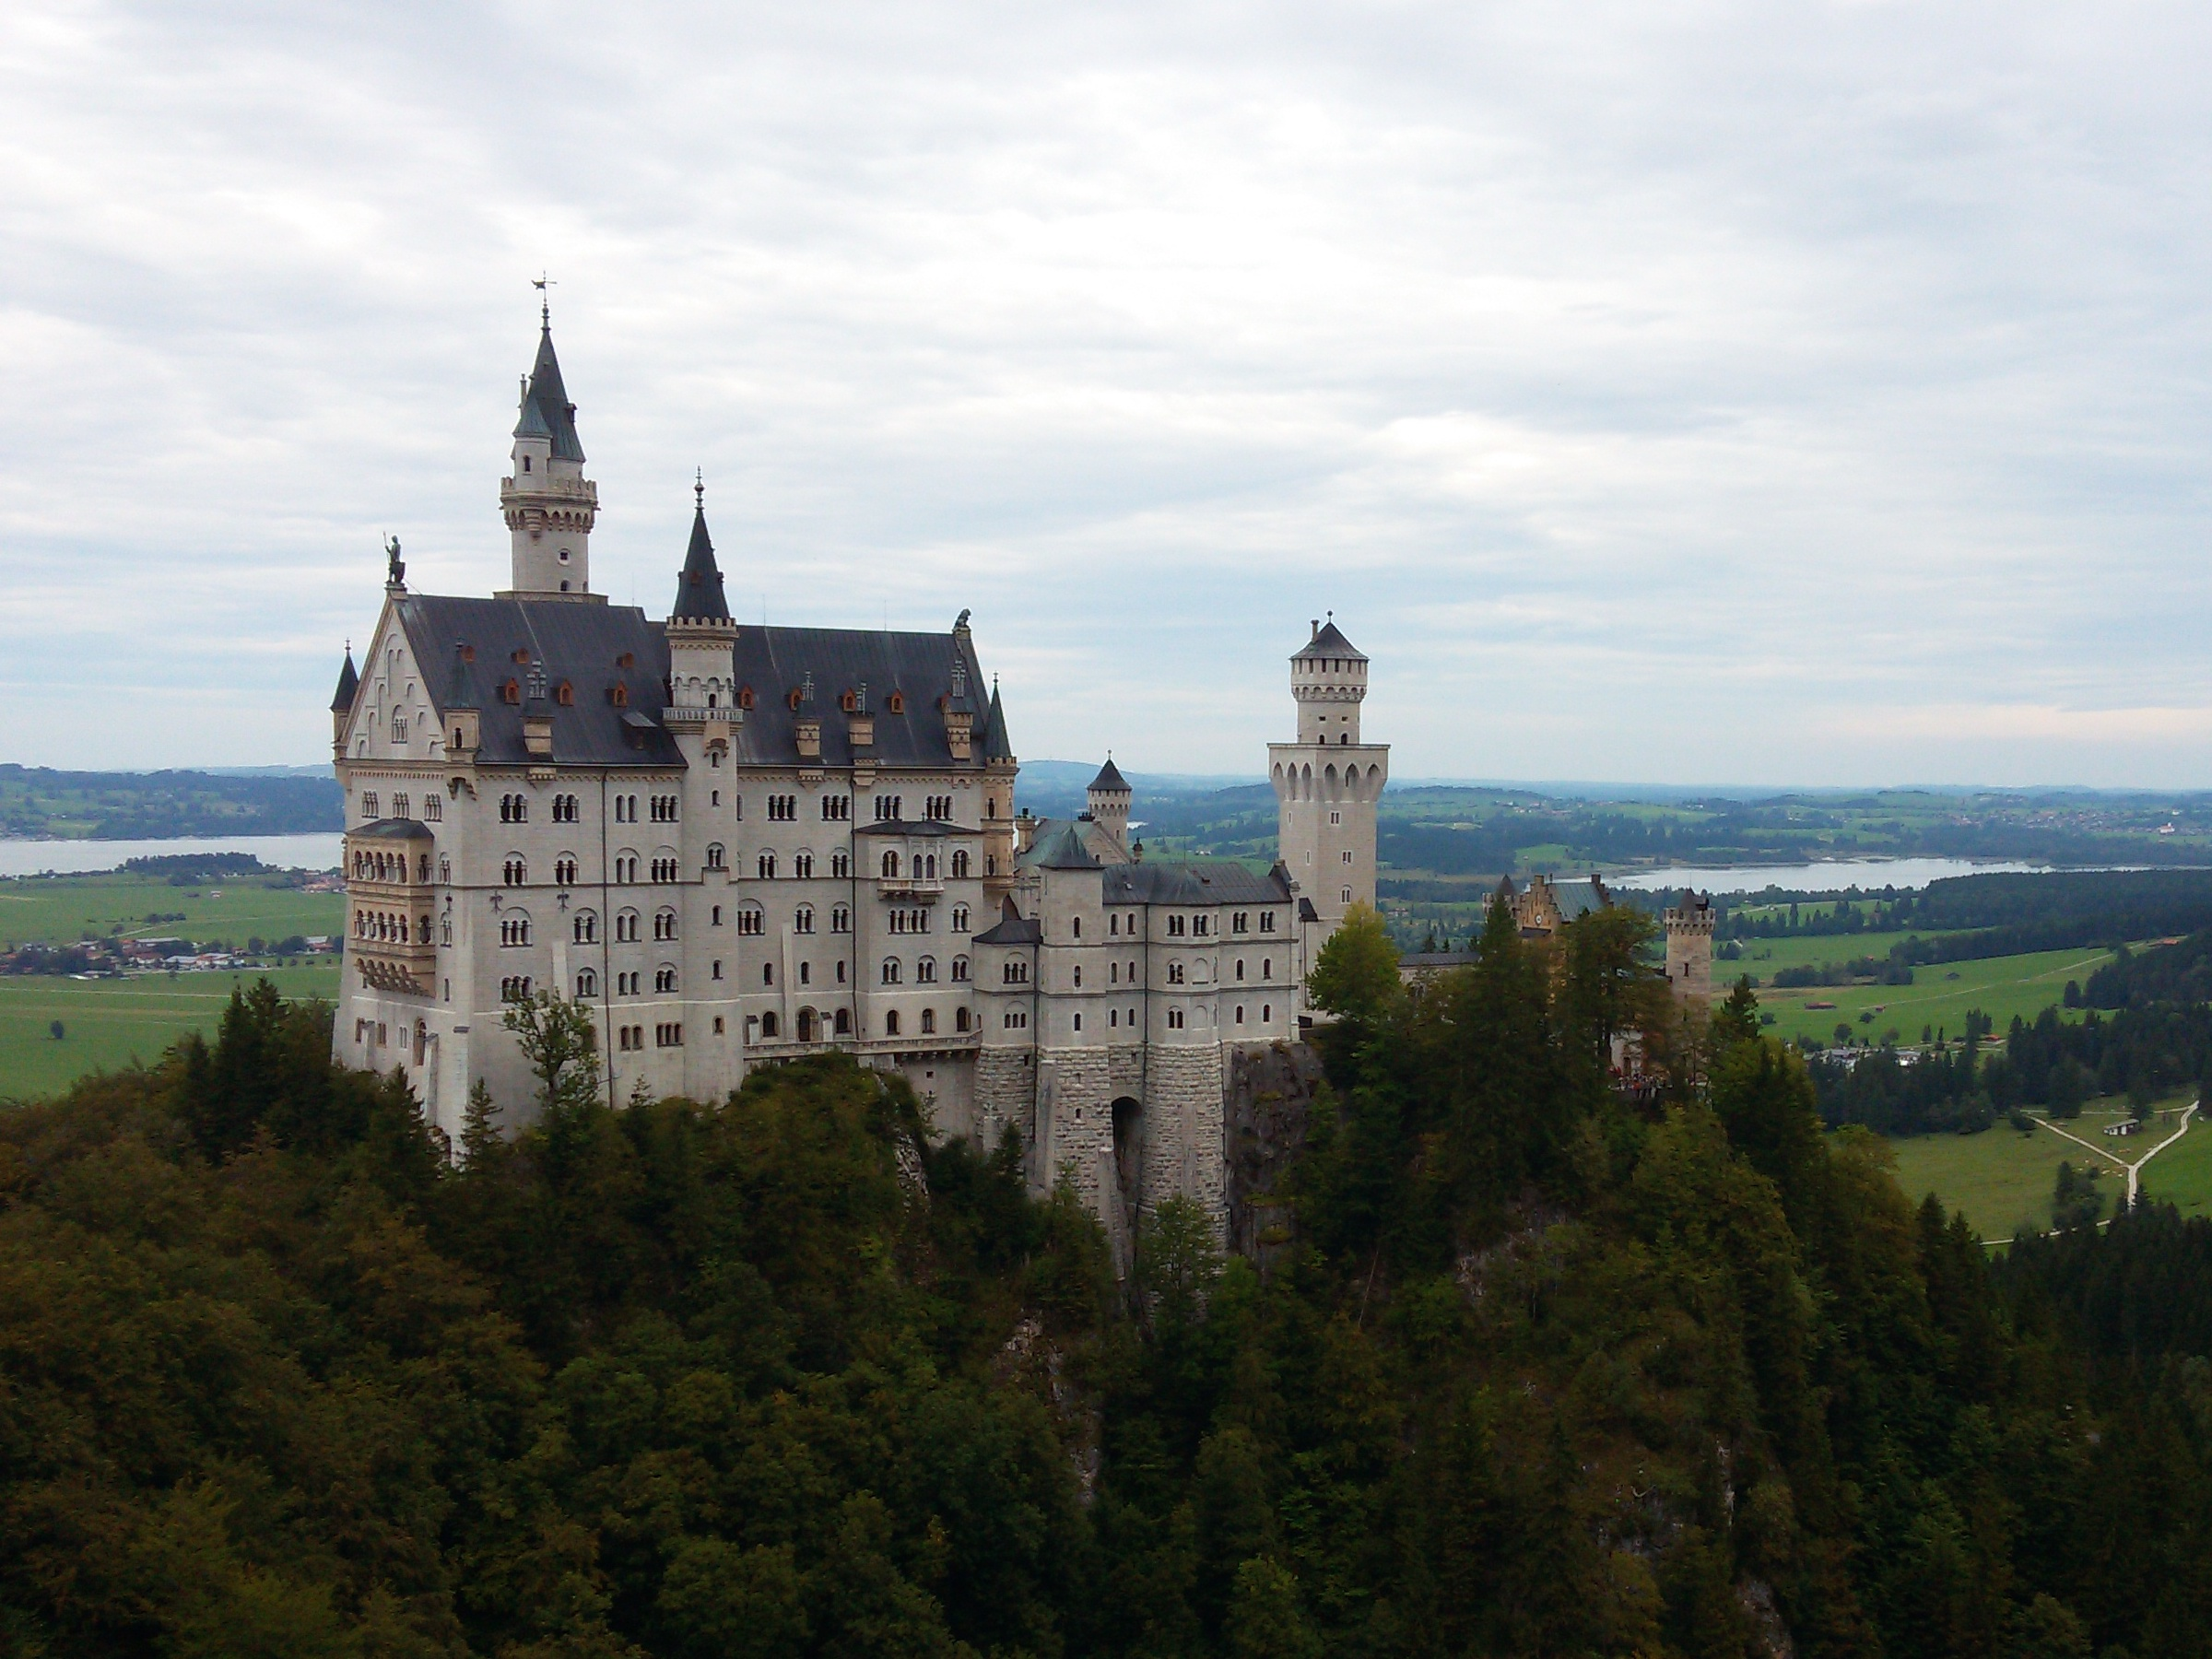
\includegraphics[width=0.8\textwidth]{castle0.jpg}
    \captionsetup{labelformat=empty}
    \caption{Малюнак \cursection.\arabic{figure}: зыходная выява}
    \label{fig:sift0}
\end{figure}

\begin{figure}[t]
    \centering
    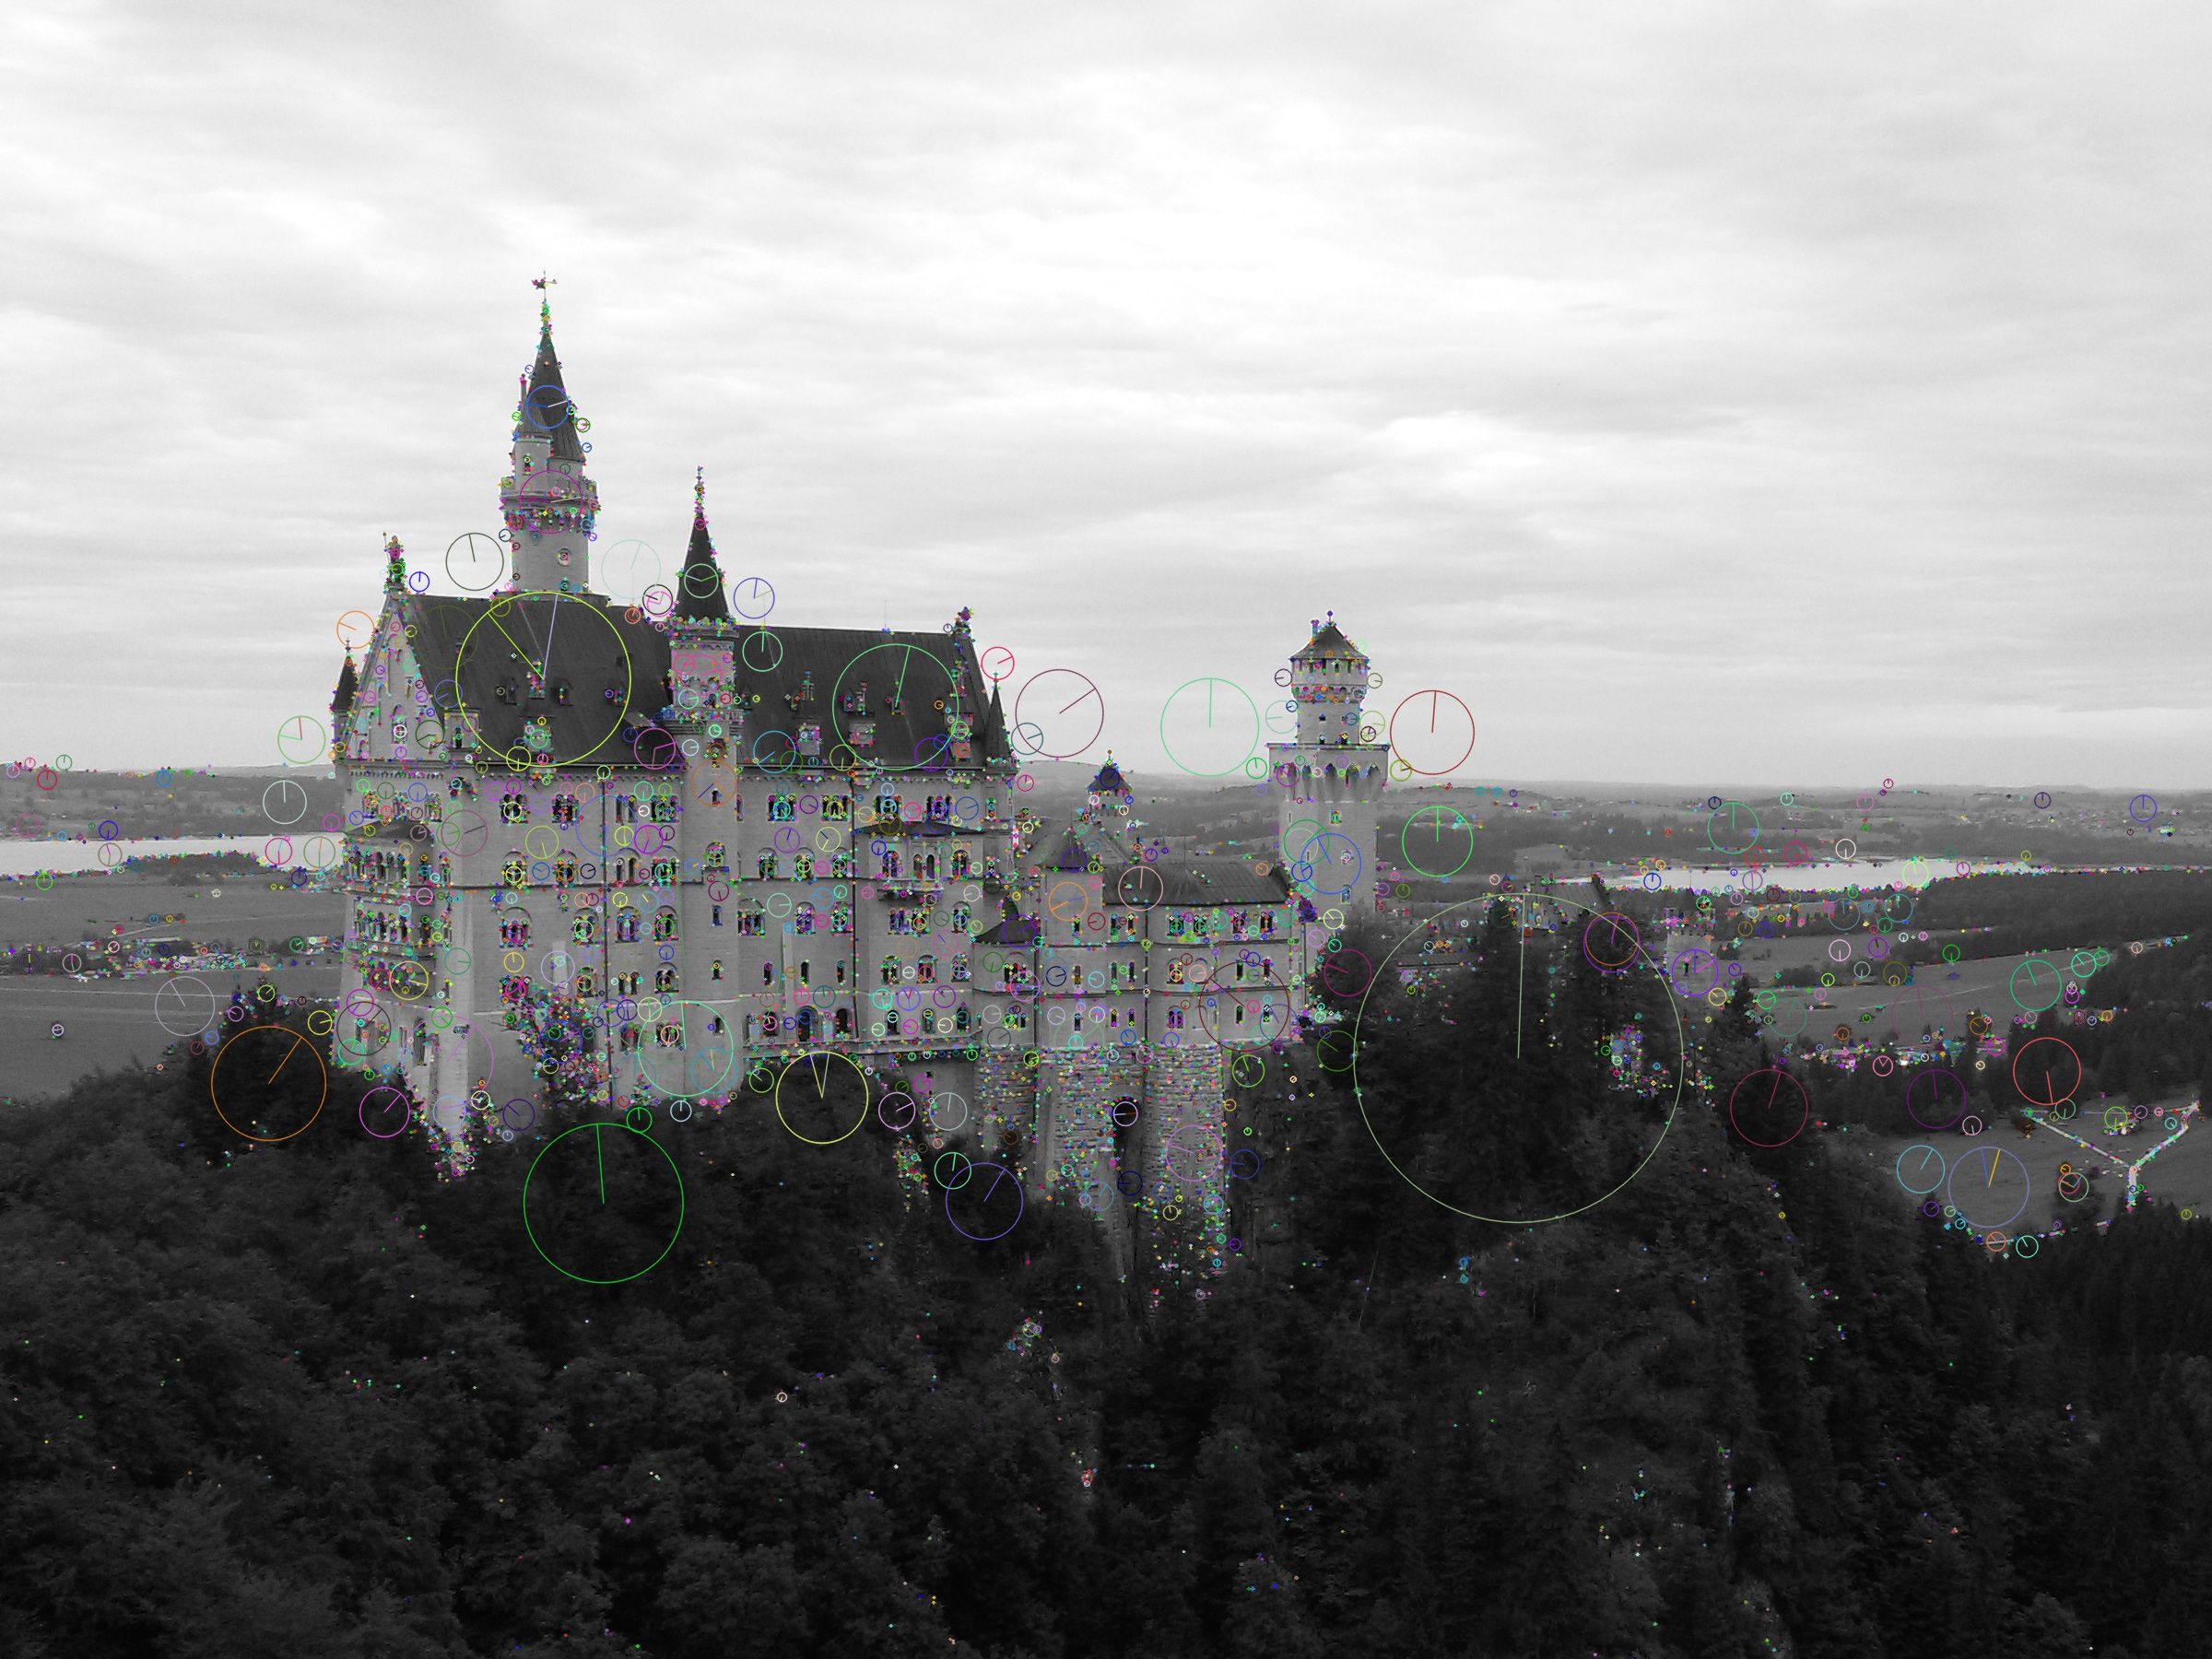
\includegraphics[width=0.8\textwidth]{castle0_sift.jpg}
    \captionsetup{labelformat=empty}
    \caption{Малюнак \cursection.\arabic{figure}: выява з нанесенымі ключавымі кропкамі (SIFT)}
    \label{fig:sift1}
\end{figure}

\vspace{5mm}

Ніжэй прыведзенае кароткае апісанне найбольш распаўсюджаных дэтэктараў ключавых кропак і спосабаў іх апісання.

\renewcommand{\nextTitle}{2.3.1 Апісанне некаторых распаўсюджаных дэтэктараў і дэскрыптараў}
\addcontentsline{toc}{subsubsection}{\nextTitle}
\subsubsection*{\nextTitle}

\vspace{5mm}

Дэтэктар \textbf{FAST} (\textit{Features from Accelerated Segment Test}) \cite{fast-paper}.
Як вынікае з назвы, асноўнай перавагай дэтэктара
з'яўляецца ягоная хуткасць, што асабліва важна ў выпадку, калі дадзеныя паступаюць
і патрабуюць апрацоўкі ў рэжыме рэальнага часу і абмежаваных рэсурсаў.
Найлепшым прыкладам будуць SLAM-прыкладанні (\textit{Simultaneous Localization and Mapping}),
у якіх у рэжыме рэальнага часу адбываецца ацэнка месцазнаходжання і пошук яго на мапе;
SLAM-прыкладанні часта знаходзяць прымяненне на мабільных прыладах, у тым ліку на БПЛА.

FAST з'яўляецца алгарытмам ``пошуку вуглоў'' (англ. \textit{corner detector}):
кропка з'яўляецца ключавой, калі ў маленькіх ваколіцах пікселя алгарытму атрымліваецца
распазнаць адпаведны шаблон, іншымі словамі ``вугал''.
Дадатковая аптымізацыя адбываецца з дапамогай метадаў машыннага навучання.

Даследаванні паказваюць, што ён у некалькі разоў хутчэйшы за іншыя існуючыя алгарытмы пошука ключавых кропак на аснове
вылучэння вуглоў, але, у сваю чаргу, ён недастаткова ўстойлівы да моцна зашумленых выяваў.

\vspace{5mm}

Дэскрыптар і дэтэктар \textbf{SIFT} \cite{sift-paper} быў прадстаўлены ў 2004 годзе і
па стане на сёння з'яўляецца адным з найбольш распаўсюджаных.
Важнымі характарыстыкамі алгарытмамі з'яўляецца ўстойлівасць да масштабавання і
змянення арыентацыі выявы, яе афінных пераўтварэнняў
і зашумленых варыянтаў. Яскрава выраджаная характэрнасць ключавых кропак дазваляе
паспяхова шукаць адпаведнасці паміж
рознымі выявамі. У \cite{sift-paper}, апроч апісання спосаба вымання ключавых кропак
і фармата дэскрыптара, апісваюцца тэхнікі для
эфектыўнага пошука адпаведнасцяў паміж выявамі з SIFT дэскрыптарамі,
а таксама алгарытмы эфектыўнага распазнавання патэрнаў.
Такая завершанасць даследавання алгарытма дае яму вялікую перавагу перад
іншымі і моцна паспрыяла ягонаму распаўсюду.
SIFT дэскрыптарам з'яўляецца рэчаісны вектар размернасці 128.

На малюнку \cursection.\ref{fig:sift1} можна бачыць візуалізацыю знойдзеных
алгарытмам SIFT ключавых кропак па пачатковым малюнку \cursection.\ref{fig:sift0}.

Дэскрыптар і дэтэктар \textbf{SURF} \cite{surf-paper} быў упершыню апублікаваны ў 2006 годзе
і пачаткова ідэя стварэння заключалася ў стварэнне ``больш хуткага'' SIFT-а.
Ён таксама з'яўляецца ўстойлівым да змены масштаба і паварота, можа быць паспяхова прыменены
для размытых выяваў; разам з тым, выкарыстанне SURF-а абмежаванае,
калі мы маем справу са зменамі ў вугле назірання. Дэскрыптар SURF
можа быць як размернасці 64, так і 128 (як SIFT).

Звернем увагу на тое, што і SIFT і SURF з'яўляюцца запатэнтаванымі алгарытмамі і,
негледзячы на вялікую колькасць рэалізацыяў з адкрытым
зыходным кодам, іх выкарыстанне ў камерцыйных прадуктах абмежаванае.
У сваю чаргу, алгарытм ORB прапрыетарным не з'яўляецца.

\vspace{5mm}

Дэскрыптар і дэтэктар \textbf{ORB} (\textit{Oriented FAST and Rotated BRIEF}) \cite{orb-paper}
з'яўляецца своеасаблівай камбінацыяй ключавых кропак FAST і дэскрыптара BRIEF.
Мэтай стварэння ORB было пераўзысці SIFT у хуткасці (нават ахвяруючы надзейнасцю і дакладнасцю)
у сувязі з распаўсюдам мабільных маламагутных прыладаў. Дэскрыптары маюць выгляд бінарных радкоў.
Адпаведнасці паміж ORB дэскрыптарамі эфектыўна могуць быць знойдзеныя з дапамогай LSH (Locality-sensitive hashing).

\vspace{5mm}

Дэскрыптар \textbf{BRIEF} (\textit{Binary Robust Independent Elementary Features}) \cite{brief-paper}
стаў адным з першых дэскрыптараў, якія апісываюць ключавыя кропкі
з дапамогай бінарных радкоў (SIFT альбо SURF, напрыклад, выкарыстоўваюць вектары
з рэчаіснымі лікамі якія, у большасці выпадкаў, пасля ўсё адно ў мэтах эфектыўнасці
фарматуюцца ў бінарныя радкі, што дазваляе выкарыстоўваць эфектыўную адлегласць Хэмінга).

\vspace{5mm}

Дэскрыптар і дэтэктар \textbf{BRISK} (\textit{Binary Robust Invariant Scalable Keypoints})
\cite{brisk-paper} ствараўся як альтэрнатыва вышэйзгаданым SIFT i SURF,
хуткасць працы якога дасягаецца праз выкарыстанне новага, заснаванага на FAST, дэтэктара
ў камбінацыі з бінарным дэскрыптарам.

\vspace{5mm}

Звернем увагу на тое, што некаторыя алгарытмы спалучаюць у сабе адразу як пошук ключавых кропак, так і падлік іх
дэскрыптараў. У агульным выпадку гэты працэс можа быць яўна падзелены: на мностве ключавых кропак атрыманых любым з дэтэктараў
можа быць запушчаны алгарытм, які для кожнай кропцы паставіць у адпаведнасць дэскрыптар вызначанага фармата.
На практыцы, некаторыя пары дэтэктара і дэскрыптара спалучаюцца добра і заўжды выкарыстоўваюцца разам, некаторыя сумяшчаюцца
вельмі кепска. Большасць алгарытмаў, якія знайшлі шырокае прымяненне, апісываюць адразу спосаб дэтэкцыі і апісання і ўтвараюць
такім чынам закрытую сістэму, раздзяленне якой не прыводзіць да добрых вынікаў.

Даследванне спалучальнасці разам разнастайных дэтэктараў і дэскрыптараў праводзіліся мной у рамках
курсавой працы.

\renewcommand{\nextTitle}{2.4 Спалучэнне простых метадаў і метадаў, заснаваных на ключавых кропках}
\addcontentsline{toc}{subsection}{\nextTitle}
\subsection*{\nextTitle}

\vspace{5mm}

Вядомыя эфектыўныя алгарытмы, якія спалучаюць у сабе простыя метады і метады,
заснаваныя на выманні асаблівасцяў. Найбольшы распаўсюд такія алгарытмы знайшлі
ў задачах апрацоўкі плыні дадзеных (відэаплыня, апрацоўка дадзеных у рэальным часе з БПЛА),
калі алгарытм будуе мапу мясцовасці і шукае сваё месцазнаходжанне ў рэальным часе.

Напрыклад, у \cite{Forster2014ICRA} яўны пошук асаблівасцяў выклікаецца толькі калі
новы кадр запускае ініцыялізацыю новых трохмерных кропак у прасторы, іначай
выкарыстоўваюцца простыя метады якія, у сваю чаргу, няяўна даюць адпаведнасці паміж кропкамі,
пазначанымі раней у якасці асаблівых.

\renewcommand{\nextTitle}{2.5 Пошук адпаведнасцяў паміж ключавымі кропкамі}
\addcontentsline{toc}{subsection}{\nextTitle}
\subsection*{\nextTitle}

Пошук асаблівых кропак і падлік адпаведных дэскрыптараў з'яўляецца, вядома ж,
толькі падрыхтоўчым этапам да этапа параўнання дэскрыптараў з
дзвюх выяваў і пошуку найлепшых параў (працэс матчынга, англ. \textit{feature matching}).
Не існуе ўніверсальнага спосаба, які даваў бы найлепшыя
вынікі на любым тыпе асаблівых кропак і іх дэскрыптараў: для кожнага набора
дэскрыптараў існуе найбольш эфектыўны спосаб пошуку адпаведнасцяў.
Таксама, выбар алгарытма залежыць ад пастаўленых намі задачаў і расстаўленых прыарытэтаў:
ці нам найважнейшая хуткасць ці дакладнасць, ці дастаткова нам толькі $n$ найлепшых супадзенняў
ці мы хочам атрымаць усе знойдзеныя. Важным пытаннем з'яўляецца вызначэнне парога,
калі знойдзеная пара дэскрыптараў з'яўляецца заведама хібнай.

\begin{figure}[h]
    \centering
    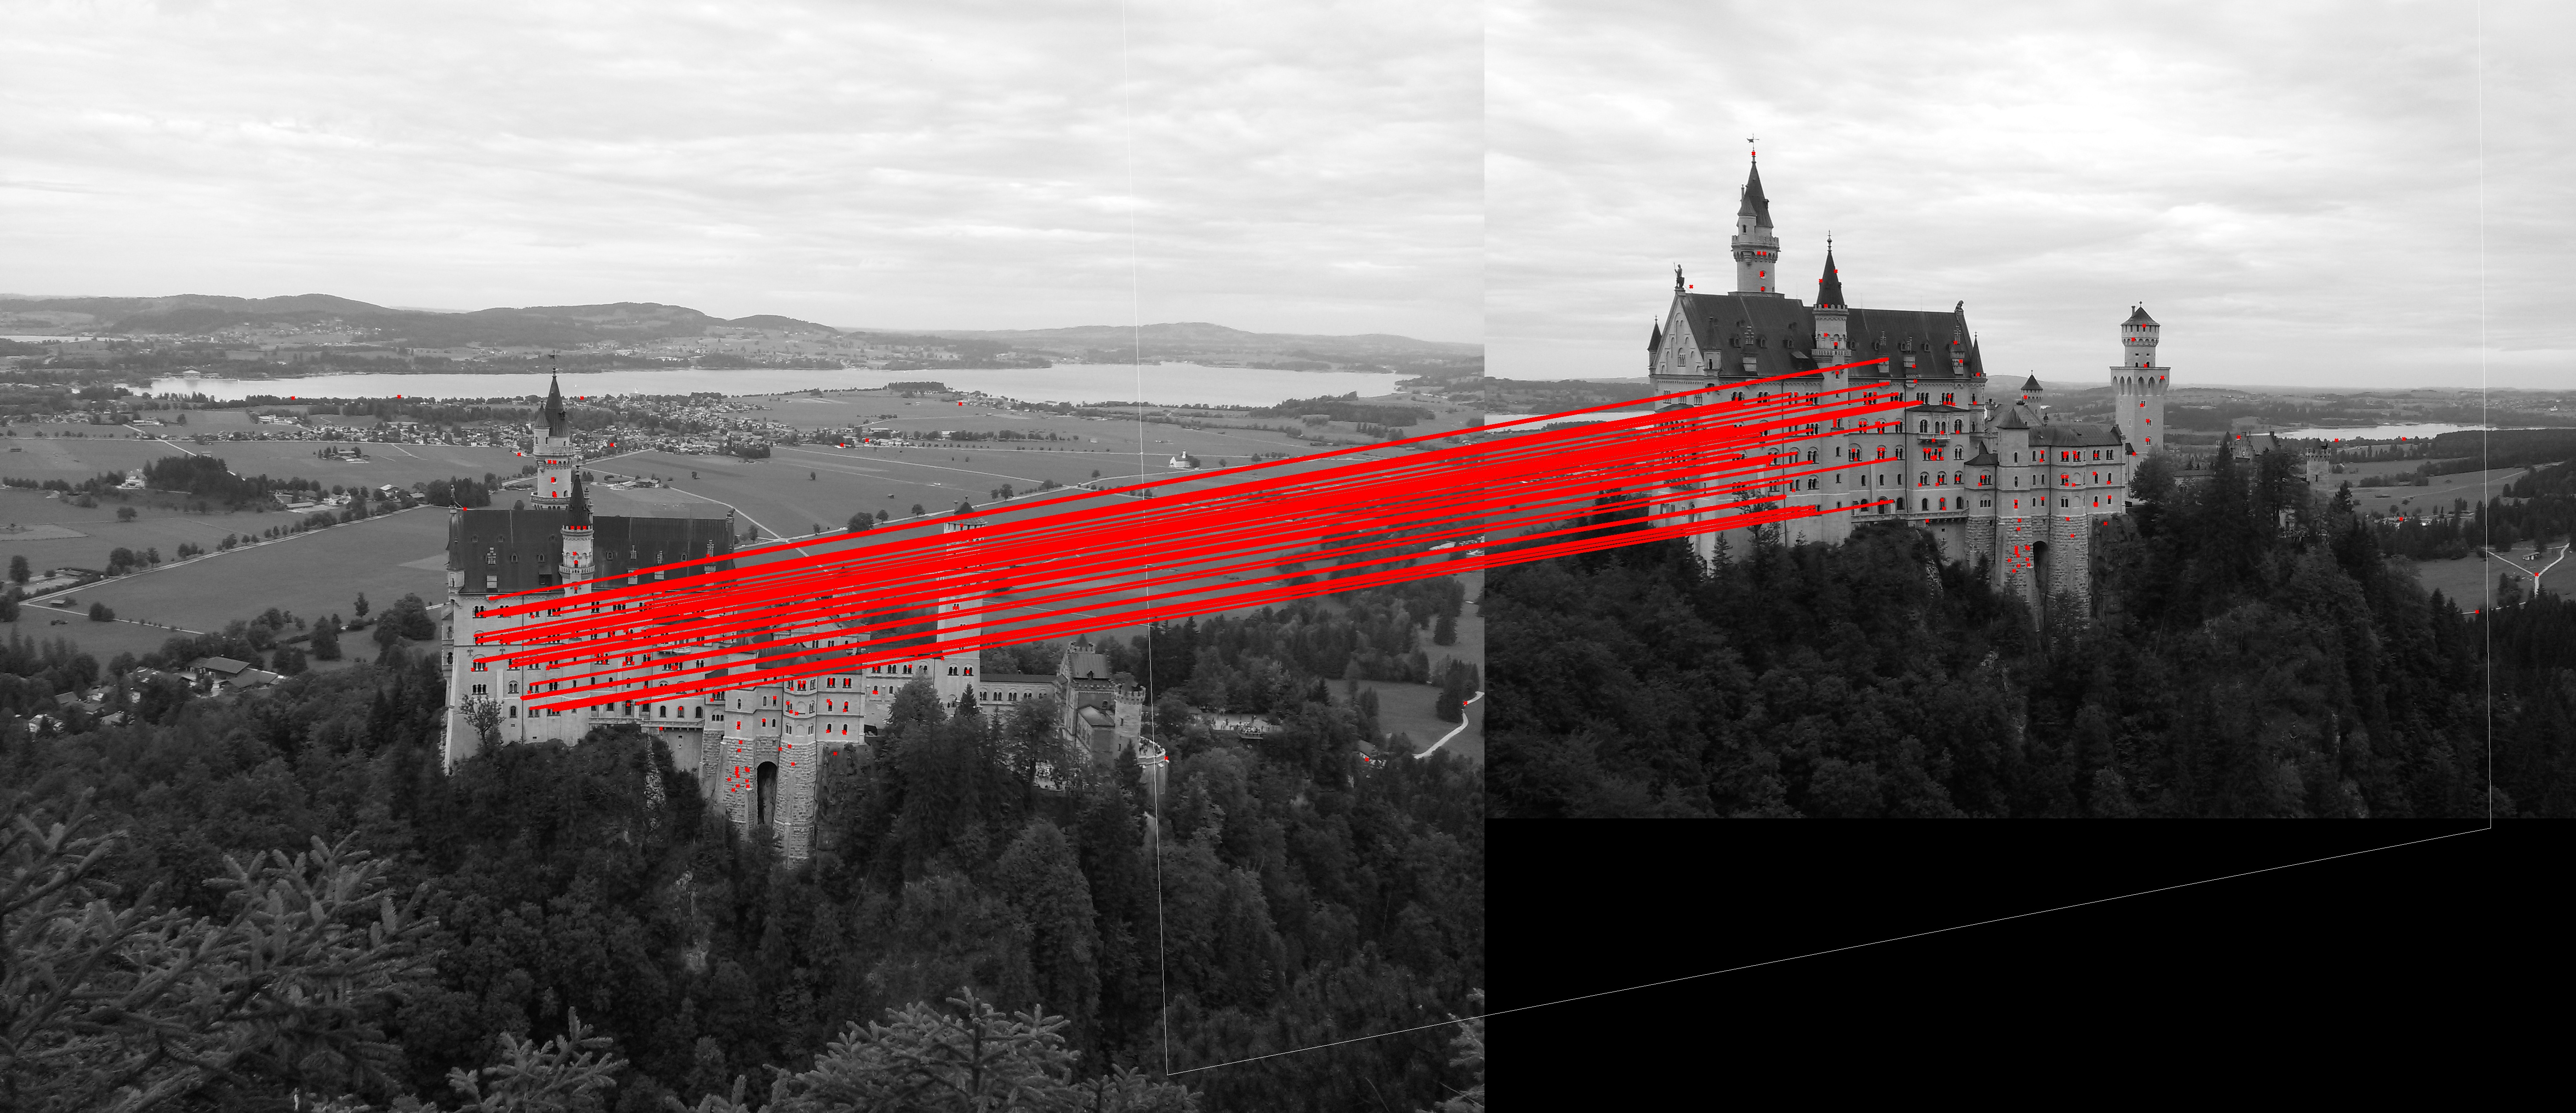
\includegraphics[width=1.0\textwidth]{castle_matches.jpg}
    \captionsetup{labelformat=empty}
    \caption{Малюнак \cursection.\arabic{figure}: вынік пошуку адпаведнасцяў паміж ключавымі кропкамі}
    \label{fig:matches}
\end{figure}

Самым простым спосабам знайсці адпаведнасці паміж дэскрыптарамі з дзвюх розных выяваў
з'яўляецца просты пералік усіх магчымых параў, падлік нормы (L2, Хэмінга, альбо любой іншай)
і сартыроўка ўсіх параў па ўзрастанні значэнняў адлегласцяў (гэтак званы Brute-Force Matcher).
Такі спосаб з'яўляецца простым у рэалізацыі, беспамылковым, але вельмі марудным.
Практычнае прымяненне ва ўмовах апрацоўкі плыняў дадзеных альбо
пры пост-апрацоўцы вялікіх набораў дадзеных часта немагчымае.

Для выпадкаў, калі дакладнасцю можна ахвяраваць на карысць хуткасці (напрыклад, у працы з БПЛА хуткасць апрацоўкі
грае першасную ролю), былі вынайдзеныя і іншыя алгарытмы пошуку адпаведнасцяў.

Метады, пра якія ідзе гаворка, маюць агульную назву \textit{метадаў набліжанага пошуку бліжэйшых суседзяў}
(англ. \textit{Approximate Nearest Neighbors}). Падлічаныя намі дэскрыптары з'яўляюцца звычайным мноствам вектароў,
на якім зададзеныя суадносіны адлегласці. У практычнай частцы такія метады будуць выкарыстоўвацца.
Для дэскрыптараў з рэчаіснымі вектарамі (SIFT, SURF) гэта будзе метад заснаваны на k-мерных дрэвах
(англ. \textit{k-dimensional trees}), для бінарных дэскрыптараў - Locality-sensitive Hashing (LSH) - імавернасны
метад паніжэння размернасці дадзеных.

На малюнку \cursection.\ref{fig:matches} можна бачыць нанесеныя простыя лініі, якія злучаюць кропкі,
адпаведныя адной і той жа кропцы прасторы.
Дэскрыптары былі падлічаныя алгарытмам SIFT.

\renewcommand{\nextTitle}{2.6 Фармальная пастаноўка задачы рэканструкцыі}
\addcontentsline{toc}{subsection}{\nextTitle}
\subsection*{\nextTitle}

\vspace{5mm}

Задача аднаўлення трохмерных каардынатаў кропак па наборы выяваў,
зробленых з розных ракурсаў і пазіцыяў, атрымала агульную назву
задачы пучковай аптымізацыі (англ. {\bf bundle adjustment}).
Задача заключаецца ў мінімізацыі памылкі функцыянала, які задае суадносіны паміж
мноствам кропак прасторы і праекцыямі гэтых кропак. Строга гэта можа быць запісана як:

\begin{equation} \label{eq:bundle-adjustment}
    \min_{a_j, b_i} \sum_{i=1}^{n} \sum_{j=1}^{m} v_{ij}d(Q(a_j, b_i), x_{ij})^2
\end{equation}

\vspace{4mm}

дзе:\\
$n$ - колькасць кропак у трохмернай прасторы, якія бачныя хаця б на адным фотаздымку,\\
$m$ - колькасць выяваў (колькасць камер),\\
$x_{ij}$ - праекцыя кропкі $i$ на выяву $j$,\\
$v_{ij}$ - дваічная зменная, якая вызначае, ці бачная кропка $i$ на выяве $j$,\\
$a_{j}$ - вектар параметраў камеры $j$,\\
$b_{i}$ - набліжэнне для кропкі $i$ прасторы,\\
$Q(a_j, b_i)$ - функцыя пошуку праекцыі кропкі $i$ на выяву $j$,\\
$d(x, y)$ - Эўклідава адлегласць паміж кропкамі $x$ i $y$.

\vspace{4mm}

Мінімізаваўшы памылку функцыянала, мы знойдзем найлепшае магчымае набліжэнне для
параметраў камераў $a_{j}$ і кропак трохмернай прасторы $b_{i}$,
што дасць нам магчымасць зрабіць візуалізацыю мадэлі, што і з'яўляецца нашай мэтай.

Дадзеная задача можа рашацца як агульнымі падыходамі да мінімізацыі функцыяналу,
так і спецыяльна распрацаванымі алгарытмамі, якія ўлічваюць разрэджаную структуру матрыцы,
якая апісвае функцыянал, такім чынам эфектыўна рашаючы задачу пучковай аптымізацыі.
Алгарытмам, які атрымаў найбольшы распаўсюд пры практычнай рэалізацыі,
з'яўляецца алгарытм Левенберга-Марквардта (англ. \textit{Levenberg–Marquardt algorithm, LMA}).
Гэта ітэратыўны алгарытм рашэння задачы мінімізацыі нелінейнага функцыянала спосабам
найменшых квадратаў (англ. \textit{non-linear least squares problem}).

\newpage

\begin{center}
    \renewcommand{\nextTitle}{ГЛАВА 3. SLAM-АЛГАРЫТМЫ}
    \addcontentsline{toc}{section}{\nextTitle}
    \section*{\nextTitle}
\end{center}

\vspace{5mm}

\renewcommand{\cursection}{3}
\setcounter{figure}{0}

\renewcommand{\nextTitle}{3.1 Асноўныя звесткі}
\addcontentsline{toc}{subsection}{\nextTitle}
\subsection*{\nextTitle}

\vspace{5mm}

Задача адначасовай лакалізацыі і пошуку на мапе (англ. \textit{Simultaneous Localization and Mapping, SLAM})
спалучае ў сабе выкарыстанне разнастайных датчыкаў (лазерныя сканеры, RGB альбо RGB-D
камеры і іншае) з мэтай ацэнкі пазіцыі робата/БПЛА ў прасторы і адначасовай пабудовы мапы мясцовасці.
Задача фармулюецца як для двухмерных, так і для трохмерных асяроддзяў: нас цікавіць
трохмерная задача, тым больш што двухмерная версія задачы лічыцца вырашанай. З адначасовасці
пабудовы мапы і ацэнкі пазіцыі ў прасторы вынікае патрабаванне да алгарытма працаваць у рэальным часе,
што накладае асаблівыя патрабаванні да алгарытмаў і абсталявання, на якім алгарытмы запускаюцца.

Сваё найбольшае развіццё рашэнне SLAM задачы атрымала ў апошнія дзесяцігоддзі. Даследванне
задачы можна ўмоўна падзяліць на тры этапы (прапанаваныя ў \cite{DBLP:journals/corr/CadenaCCLSN0L16},
\cite{Li2016RealtimeSL}). Першы перыяд, прыблізна 1986-2004, можна назваць ``класічным''.
У гэтыя часы асноўным накірункам працы па рашэнні задачы была імавернасная фармуліроўка
і падыходы, заснаваныя на фільтрах. У другі перыяд, 2004-2015, былі даследаваныя асноўныя
ўласцівасці, такія як назіральнасць, збежнасць і ўзгодненасць алгарытмаў. У гэты час былі
праведзеныя цесныя аналогія з існуючымі падыходамі ў галіне камп'ютарнага зроку,
была ствароная вялікая колькасць рэалізацыяў з адкрытым зыходным кодам, з'яўляліся першыя спробы
прымянення SLAM у практычных прыкладаннях.

Мяркуецца, што на трэці этап распрацоўка перайшла зусім нядаўна, у апошнія гады: гэта звязваюць
з публікацыямі такіх алгарытмаў, як ORB-SLAM ці LSD-SLAM, якія па сваёй
функцыянальнасці моцна пераўзыходзяць любыя ранейшыя публікацыі. Прынцыпы працы гэтых алгарытмаў,
як і некаторых іншых, будуць разгледжаныя далей.

Важна успрымаць SLAM не як адзіны прапанаваны алгарытм, але як канцэпцыю. SLAM-сістэмы складаюцца са
шматлікіх частак і кожная з гэтых частак можа ўдзельнічаць у рашэнні агульнай задачы з той ці іншай эфектыўнасцю.

Для задачы рэканструкцыі паверхні SLAM-сістэма наўрад ці будзе
аптымальным рашэннем: пабудова шчыльных мадэляў у рэальным часе пакуль яшчэ застаецца
слаба вырашанай задачай. Тут і далей SLAM-сістэмы нас цікавяць сваімі выхаднымі
дадзенымі: пасля апрацоўкі дадзеных у рэальным часе захаваныя пазіцыі, павароты камераў
у часе і пабудаваная глабальная мапа могуць быць эфектыўна выкарыстаныя ў якасці
ўваходных дадзеных афлайн алгарытма, падвышаючы ягоную дасканаласць і хуткасць працы.

Як вынікае з назвы, алгарытмы рашаюць дзве асноўныя задачы: лакалізацыю і пошук на мапе.
На першых этапах даследавання задачы разглядаліся асобна, але з цягам часу стала зразумела,
што задачы цесна звязаныя паміж сабой і рашэнне адной з іх моцна дапамагае ў рашэнні іншай. Мапа патрэбная для
эфектыўнага пошуку пазіцыі ў прасторы, у той жа час з ацэнкай становішча мапа сабірае больш дадзеных
і становіцца больш дакладнай.

Большасці сучасных SLAM-алгарытмаў прысутная магчымасць замыкаць цыклы (\textit{loop closure}) -
знаходзіць аб'екты, якія сустракаліся ў прасторы раней у межах таго ж пралёту/праходу асяроддзя,
распазнаваць іх у якасці \textit{знаёмых} і глабальна ўдасканальваць мапу на падставе факта
паўторна сустрэнутага аб'екта. Падыход добра паўплываў на якасць працы мноства алгарытмаў
і зарэкамендаваў сябе адпаведным чынам -- прычына поспеху ў надзейнасці вонкавых сістэм, здольных
успрымаць відэаплыню і знаходзіць аб'екты незалежна ад асноўных плыняў алгарытма.

Разгледзім асноўныя этапы падрабязней.

\renewcommand{\nextTitle}{3.2 Ключавыя паняцці і падыходы}
\addcontentsline{toc}{subsection}{\nextTitle}
\subsection*{\nextTitle}

\vspace{5mm}

\renewcommand{\nextTitle}{3.2.1 Лакалізацыя}
\addcontentsline{toc}{subsubsection}{\nextTitle}
\subsubsection*{\nextTitle}

Пры руху пазіцыя БПЛА ў дыскрэтным часе задаецца матрыцай $T \in \mathbb{R}^{4\times4}$.
Паслядоўнасць такіх матрыцаў -- траекторыя пралёту. Лакалізацыя - пошук такой матрыцы ў вызначаны момант часу.
Для адкрытых прастораў задача была часткова вырашаная з запускам GPS - глабальнай сістэмы
пазіцыянавання; у прасторах, дзе GPS недаступны, таксама можа выкарыстоўвацца вонкавае
абсталявання для лакалізацыі, што часта з'яўляецца непрактычным альбо дарагім рашэннем.
Выкарыстанне датчыкаў, усталяваных на БПЛА, для лакалізацыі ў прасторы, робіць падыходы
да рашэння задачы больш універсальнымі. Лакалізацыю з дапамогай толькі камераў часам
таксама называюць візуальнай адаметрыяй (англ. \textit{Visual Odometry}). Надзейныя механізмы
лакалізацыі аўтаномных БПЛА асабліва важныя праз знаходжанне БПЛА ў паветры і
немагчымасць спыніцца, у адрозненні на наземных робатаў.

\renewcommand{\nextTitle}{3.2.2 Пошук на мапе}
\addcontentsline{toc}{subsubsection}{\nextTitle}
\subsubsection*{\nextTitle}

Ёсць некалькі важных аспектаў пабудовы мапы. Па-першае, мапа выкарыстоўваецца для пракладкі
маршрутаў і лакалізацыі перашкодаў -- асноўныя элементы для аўтаномнай навігацыі. Па-другое --
мапа на выхадзе можа быць цікавая сама па сабе: яна можа пасля выкарыстоўвацца для візуалізацыі пралёта
па мясцовасці альбо як уваходныя дадзеныя для алгарытмаў афлайн-рэканструкцыі, для распазнавання
аб'ектаў і гэтак далей. Трэці і, магчыма, самы важны аспект у дачыненні да канцэпцыі SLAM --
добра пабудаваная мапа дазваляе лакалізаваць БПЛА ў прасторы.

Адзін з важных аспектаў пошука на мапе -- магчымасць пошуку элементаў, месцаў,
якія былі наведаныя і пабачаныя раней.
Гэты працэс называецца \textit{замкненнем цыклаў} (англ. \textit{loop closure}).

\vspace{5mm}

Такім чынам, лакалізацыя і пошук на мапе не выступаюць як дзве асобныя і незалежныя
часткі алгарытма, але дапаўняюць і паляпшаюць адна адну. Пошук сябе на папярэдне пабудаванай мапе
(напрыклад, пры паўторным пралёце той жа мясцовасці) дазваляе лакалізаваць БПЛА з
якасцю, параўнальнай з якасцю пабудаванай мапы, у сваю чаргу лакалізацыя пры дапамозе
адаметрыі і старонніх датчыкаў паслядоўна ўдасканальвае мапу. Сфармуляваўшы гэтую залежнасць
іншымі словамі, пры наяўнасці дакладна вырашанай задачы альбо лакалізацыі, альбо пошуку на мапе,
іншая задача таксама можа лічыцца вырашанай.

\renewcommand{\nextTitle}{3.3 Падыходы да рэалізацыі}
\addcontentsline{toc}{subsection}{\nextTitle}
\subsection*{\nextTitle}

\vspace{5mm}

Як зазначаецца ў \cite{Li2016RealtimeSL}, архітэктура любой SLAM-сістэмы
можа быць прадстаўленая схемай з малюнку \cursection.\ref{fig:slam-architecture}. Фронтэнд выконвае
першасную апрацоўку дадзеных, якія паступаюць са знешніх датчыкаў. Для алгарытмаў,
заснаваных на пошуку асаблівых кропак, фронтэнд займаецца іх пошукам і апісаннем;
для алгарытмаў, якія працуюць непасрэдна са значэннямі пікселяў, выконваецца трэкінг паміж
кадрамі. Усе вынікі першаснай апрацоўкі пасля перадаюцца бэкэнду.

Бэкэнд, у сваю чаргу, займаецца пабудовай графа залежнасцяў, аптымізацыяй на графе.
Можна сказаць, што сёння асноўныя намаганні даследчыкаў прыкладаюцца да фронтэнду; бэкэнд
жа можна ўмоўна лічыць стандартаваным, яго задача -- аптымізацыя графа, які змяшчае інфармацыю
пра пазіцыі ключавых кадраў і залежнасці паміж імі.

Задача SLAM з выкарыстаннем адзінай камеры ў якасці сэнсара на сённяшні момант
лічыцца нявырашанай па прычыне нястачы вылічальных магутнасцяў, недахопе дадзеных
пра глыбіню выявы і складанасці пошуку і асацыяцыі паміж сабой ключавых кропак.
У некаторых сітуацыях некаторыя з вышэйзгаданых праблемаў могуць быць вырашаныя
(альбо часткова вырашаныя). Напрыклад, задача высвятлення глыбіні выявы не стаіць так
востра пры выкарыстанні стэрэакамеры, альбо калі пра манакулярную камеру вядома,
што яна глядзіць уніз (англ. \textit{downward looking camera}).

Важным крокам у рэалізацыі SLAM-алгарытмаў стала дамінаванне ідэі раздзялення лакалізацыі
і пошуку на мапе ў асобныя плыні. Упершыню практычнае прымяненне ідэя знайшла
ў сістэме PTAM (\textit{Parallel Tracking and Mapping for Small AR Workspaces}, \cite{Klein:2007:PTM:1514339.1514363}).
Лакалізацыйная плыня PTAM займаецца пошукам адпаведнасцяў у дадзеных і запускае
аптымізацыю па рухах камеры. У гэты ж час плыня з мапай калекцыянуе вынікі лакалізацыі,
трыангулюе выяўленыя асаблівасці ў трохмерныя кропкі і абнаўляе глабальную мапу.
Са з'яўленнем такога падыходу сталі відавочнымі ягоныя перавагі і амаль кожная
сучасная SLAM-сістэма пабудаваная па падобным прынцыпе.

\begin{figure}[H]
  \centering
  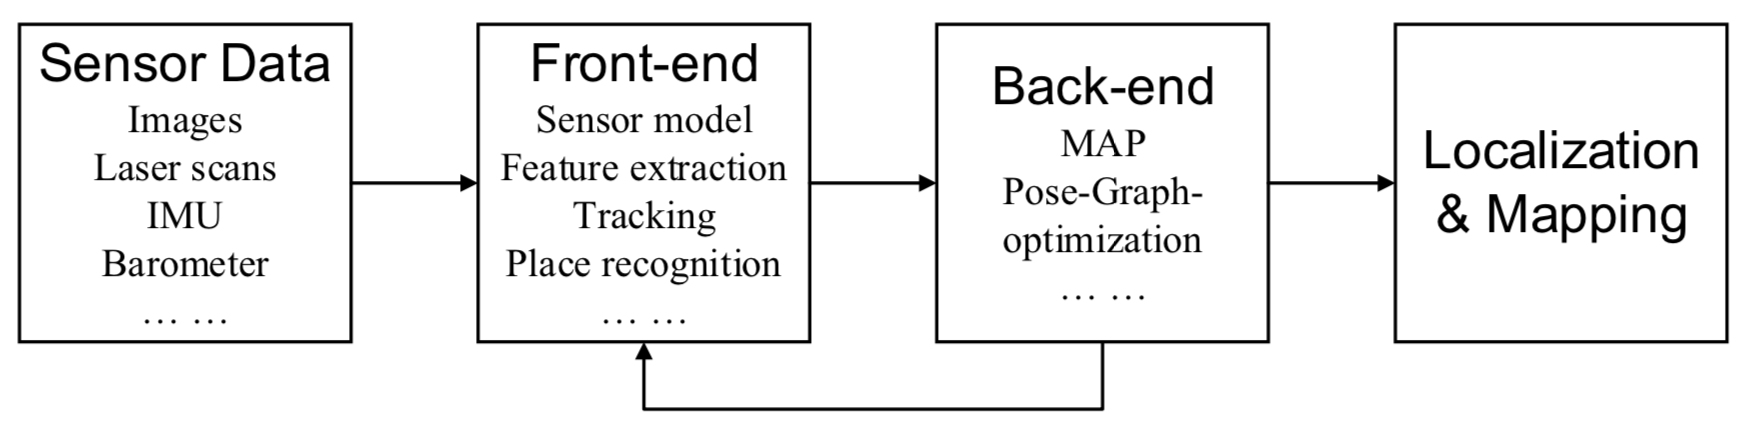
\includegraphics[width=.9\textwidth]{slam-architecture}
  \captionsetup{labelformat=empty}
  \caption{Малюнак \cursection.\arabic{figure}: высокаўзрозневая архітэктура SLAM-алгарытмаў}
  \label{fig:slam-architecture}
\end{figure}

\renewcommand{\nextTitle}{3.4 Агляд SLAM-сістэм}
\addcontentsline{toc}{subsection}{\nextTitle}
\subsection*{\nextTitle}

Далей ідзе апісанне асаблівасцяў некаторых SLAM-сістэм, якія на сённяшні дзень паказваюць найлепшыя вынікі.
Некаторыя з іх заснаваныя на пошуку асаблівых кропак (\textit{feature-based SLAM}),
другія -- на простых метадах (\textit{direct SLAM}), трэція -- камбінуюць у сабе
абодва падыхода (\textit{semi-direct SLAM}).
Да прыкладу, ORB-SLAM (\cite{murTRO2015}, \cite{murORB2}) адносіцца да першай катэгорыі
SLAM-сістэм, LSD-SLAM (\cite{engel14eccv}) -- да другой, SVO(\cite{Forster2014ICRA}) --
да трэцяй.

\renewcommand{\nextTitle}{3.4.1 ORB-SLAM}
\addcontentsline{toc}{subsubsection}{\nextTitle}
\subsubsection*{\nextTitle}

ORB-SLAM (\cite{murTRO2015}, \cite{murORB2}) -- манакулярная SLAM-сістэма,
заснаваная на пошуку асаблівасцяў на выявах (\textit{feature-based}),
спраектаваная для працы ў маленькіх і вялікіх, замкнёных і адкрытых прасторах.

Асноўныя асаблівасці:

\begin{itemize}
  \item выкарыстанне адных і тых жа ключавых кропак на ўсіх этапах працы алгарытма;
  \item чатыры асноўныя задачы, якія адначасова рашае алгарытм: трэкінг (\textit{tracking}),
  нанясенне дадзеных на мапу (\textit{mapping}), рэлакалізацыя (\textit{relocalization}),
  замкненне цыклаў (\textit{loop closing});
  \item неабмежаваны рост памераў мапы \textit{толькі} з ростам аглядаемай тэрыторыі;
  \item выкарыстанне ORB-дэскрыптараў як найлепшых па хуткасці (без ужывання GPU)
  і інварыянтнасці да зменаў у павароце і асвятленні;
  \item хуткі трэкінг і пошук на мапе на лакальных абласцях бачнасці, што дасягаецца
  праз выкарыстанне \textit{графа узаемабачнасці} (\textit{covisibility graph});
  \item новы аўтаматычны і надзейны спосаб ініцыялізацыі, які стварае пачатковыя мапы
  як для планарных, так і для непланарных паверхняў;
  \item пазбаўленне ад лішніх ключавых кадраў па стратэгіі ``выжывання наймацнейшага''
  (\textit{survival of the fittest});

  \begin{figure}[H]
    \centering
    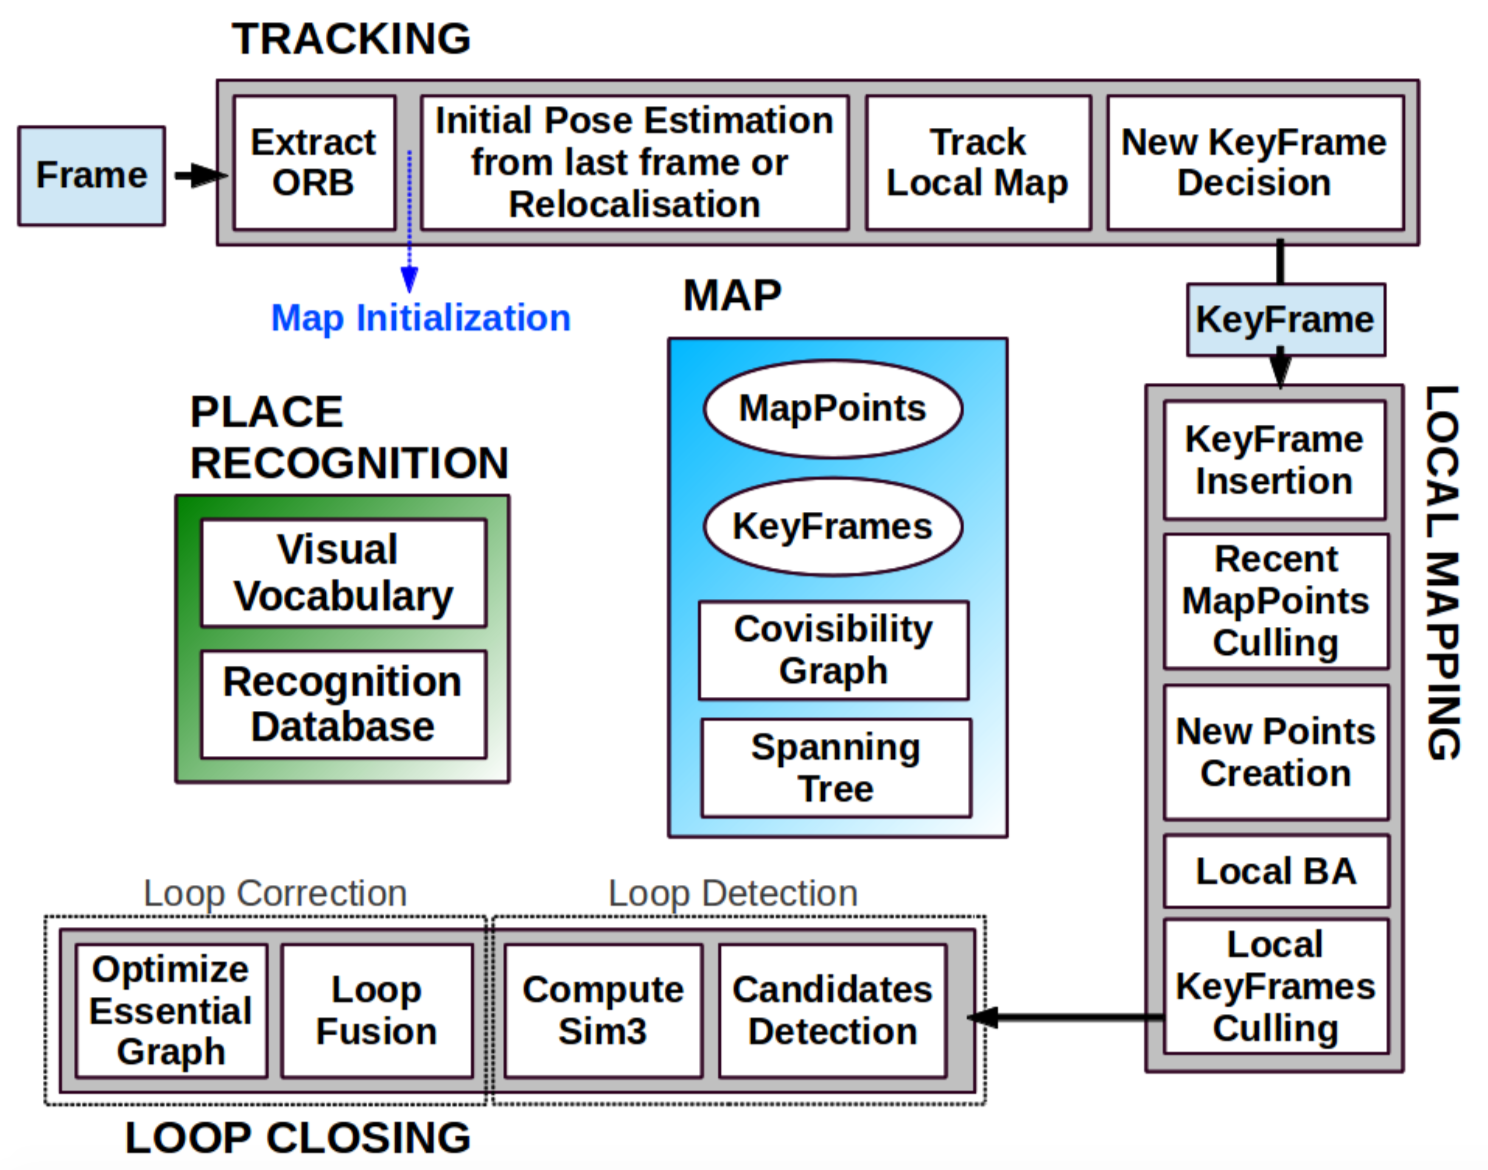
\includegraphics[width=.7\textwidth]{orb-architecture}
    \captionsetup{labelformat=empty}
    \caption{Малюнак \cursection.\arabic{figure}: архітэктура ORB-SLAM}
    \label{fig:orb-architecture}
  \end{figure}

  \item агульная схема працы алгарытма прадстаўленая на малюнку \cursection.\ref{fig:orb-architecture}.
\end{itemize}

Арыгінальная публікацыя (\cite{murTRO2015}) прыводзіла апісанне манакулярнай сістэмы,
у другой рэдакцыі алгарытма (ORB-SLAM2, \cite{murORB2}) дадалася падтрымка стэрэа і RGB-D камер.
Пра рэалізацыю варта зазначыць, што першая версія была даступная толькі пад ROS
(аперацыйная сістэма, шырока распаўсюджаная сярод робататэхнікаў),
у сваю чаргу ў другой версіі з'явіліся ўласныя сродкі візуалізацыі, здольныя працаваць незалежна.

\renewcommand{\nextTitle}{3.4.2 LSD-SLAM}
\addcontentsline{toc}{subsubsection}{\nextTitle}
\subsubsection*{\nextTitle}

У адрозненні ад разгледжанай вышэй сістэмы ORB-SLAM, заснаванай на пошуку
асаблівых кропак, LSD-SLAM (\cite{engel14eccv}) выкарыстоўвае \textit{простыя} (\textit{direct})
падыходы да працы з выявамі, то бок працуе непасрэдна са значэннямі ў пікселях.

\begin{figure}[H]
  \centering
  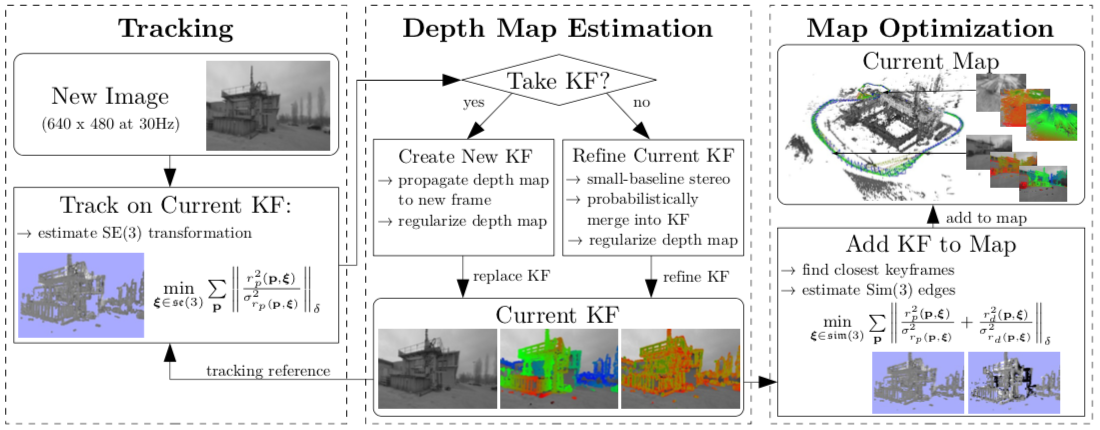
\includegraphics[width=.8\textwidth]{lsd-architecture}
  \captionsetup{labelformat=empty}
  \caption{Малюнак \cursection.\arabic{figure}: архітэктура LSD-SLAM}
  \label{fig:lsd-architecture}
\end{figure}

\begin{itemize}
  \item працуе ў рэальным часе на CPU;
  \item складаецца з трох асноўных кампанент: трэкінг, падлік набліжэння для мапы
  глыбіняў і аптымізацыя мапы;
  \item трэкінг кампанента паслядоўна апрацоўвае новыя здымкі, прымаючы да ўвагі
  папярэдні і бягучы ключавыя здымкі;
  \item другая кампанента выкарыстоўвае здымкі каб альбо палепшыць, альбо замяніць
  бягучы ключавы кадр і ацэньвае глыбіню сцэны простымі (\textit{direct})
  і імавернаснымі падыходамі;
  \item здымкі, якія канчаткова пазначаныя як ключавыя (мапа глыбіняў больш
  змяняцца не будзе) заносяцца на глабальную мапу;
  \item мапа - граф узаемаразмяшчэння ключавых кадраў. Паколькі алгарытм таксама
  ацэньвае мапы глыбіняў, то мапа, па сутнасці, ўяўляе сабой напаўшчыльную
  трохмерную рэканструкцыю паверхні;
  \item аўтары ініцыялізуюць першы ключавы кадр \textit{выпадковай} мапай глыбіняў
  з вялікімі перападамі. Сцвярджаецца, што пры значных рухах камеры ў прасторы
  ў першую секунду, першасная мапа глыбіняў будзе хутка збягацца. Аўтары прызнаюцца
  ў неабходнасці дапрацаваць гэтую частку сістэмы; пры тэставых запусках мапа
  глыбіняў для ініцыялізацыі бралася непасрэдна з датасэтаў (то бок была дакладна
  вядомая), на практыцы падобны падыход можа запатрабаваць пэўнага чалавечага ўдзелу;
  \item архітэктура сістэмы прадстаўленая на малюнку \cursection.\ref{fig:lsd-architecture}.
\end{itemize}

\renewcommand{\nextTitle}{3.4.3 SVO}
\addcontentsline{toc}{subsubsection}{\nextTitle}
\subsubsection*{\nextTitle}

У адрозненні ад папярэдніх двух прыкладаў, SVO (\textit{Semi-Direct Monocular Visual Odometry},
\cite{Forster2014ICRA}) спалучае ў сабе як пошук і апісанне ключавых кропак, так і
простыя метады, праз што і атрымаў сваю назву (\textit{Semi-Direct, паўпросты}).

\begin{figure}[H]
  \centering
  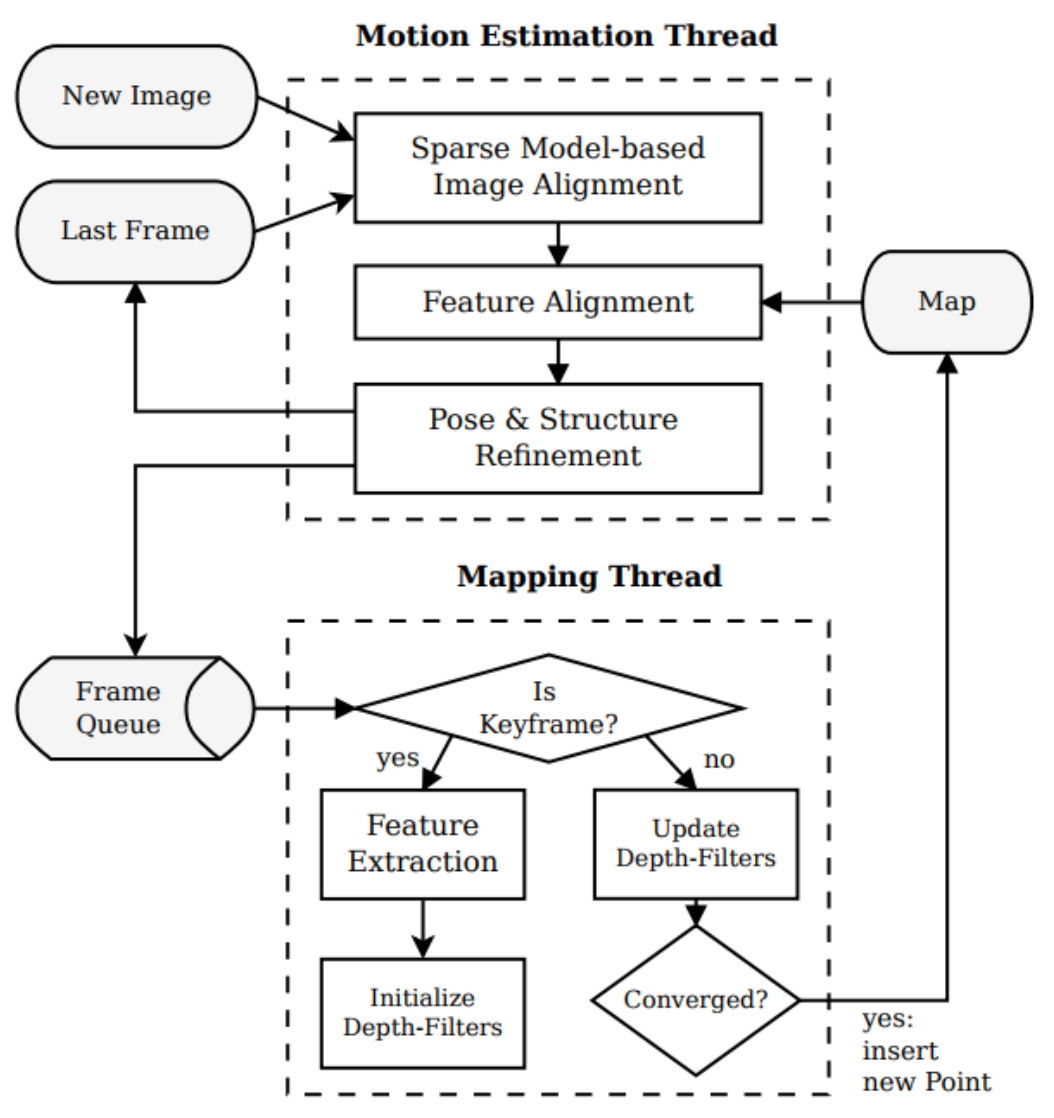
\includegraphics[width=.5\textwidth]{svo-architecture}
  \captionsetup{labelformat=empty}
  \caption{Малюнак \cursection.\arabic{figure}: архітэктура SVO}
  \label{fig:svo-architecture}
\end{figure}

\begin{itemize}
  \item спалучае ў сабе лепшае ад метадаў, заснаваных на ключавых кропках (выбар
  ключавых кадраў, сачэнне за мноствам кропак, паралельны трэкінг і пошук на мапе),
  і ад простых метадаў (хуткасць і дакладнасць);
  \item пошук адпаведнасцяў паміж ключавымі кропкамі здзяйсняецца няяўна як вынік
  прымянення простых метадаў (а не, напрыклад, matching-а);
  \item выманне ключавых кропак здзяйсняецца толькі на ключавых кадрах;
  \item пасля таго, як адпаведнасці паміж ключавымі кропкамі, а таксама пачатковая пазіцыя
  камеры ўсталяваныя, алгарытм толькі працуе з непасрэднымі значэннямі пікселяў у кропках.
  Пазіцыя камеры адносна папярэдняга кадра падлічваецца праз мінімізацыю фотаметрычнай памылкі;
  \item трохмерная кропка дадаецца на мапу толькі ў выпадку збежнасці адпаведнага
  фільтра глыбіняў, што азначае патрэбнасць у шматлікіх вымярэннях для кожнай асобнай кропкі;
  \item глыбінныя фільтры для ключавых кадраў ініцыялізуюцца сярэднім значэннем
  сярод усіх глыбінных фільтраў сцэны;
  \item свядзенне да мінімума выкідаў у вымярэннях;
  \item архітэктура сістэмы прадстаўленая на малюнку \cursection.\ref{fig:svo-architecture}.
\end{itemize}

\renewcommand{\nextTitle}{3.4.4 CNN-SLAM}
\addcontentsline{toc}{subsubsection}{\nextTitle}
\subsubsection*{\nextTitle}

Аўтары алгарытма CNN-SLAM \cite{DBLP:journals/corr/TatenoTLN17} прапаноўваюць альтэрнатыўны падыход да ацэнкі
глыбіні сцэны пры наяўнасці адзінай камеры. Найбольш класічным ў такім выпадку лічыцца
імітацыя стэрэакамеры (ацэнка глыбіні сцэны пра невялікіх рухах камеры ў прасторы), аднак такі
падыход мае пэўныя праблемы, якія не дазваляюць ягонае надзейнае выкарыстанне. Напрыклад,
падыход не прымяняльны пры паваротах у прасторы. Аўтары прапаноўваюць будаваць глыбіню,
базуючыся на адзіным кадры з дапамогай канвалюцыйных нейронных сетак
(\textit{Convolutional Neural Networks, CNN}, адсюль паходзіць назва алгарытма).
Сярод іншых асаблівасцяў алгарытма:

\begin{itemize}
    \item дазваляе абысці адно з найвялікшых абмежаванняў усіх SLAM-алгарытмаў --
    немагчымасць ацаніць рэальныя масштабы сцэны, якая аглядаецца. SLAM-алгарытмы
    заўжды даюць вынікі з дакладнасцю да масштабу, калі толькі не прымяняюцца спецыяльныя падыходы,
    якія дапамагаюць зразумець рэальныя памеры аб'ектаў. Прыкладам такога падыхода
    можа быць распазнаванне аб'ектаў і наступнае параўнанне з базай аб'ектаў,
    для якіх вядомыя іх фізічныя характарыстыкі. Зразумела, што такі падыход не дасць аніякіх
    вынікаў пры адсутнасці на сцэне хаця б аднаго аб'екта з базы;
    \item нейронная сетка навучаецца не на прыкладах з аднаго канкрэтнага асяроддзя,
    але па наборы дадзеных, які змяшчае ў сабе вельмі разнастайныя выявы. Гэта дазваляе,
    аднойчы навучыўшы SLAM-сістэму, запускаць яе ў разнастайных асяроддзях (у тым ліку --
    у незнаёмых) з аднолькавай паспяховасцю;
    \item мапы глыбіняў, згенераваныя нейроннай сеткай, хаця і глабальна карэктныя,
    даюць размытасці на вуглах, граніцах. Гэта не дазваляе выкарыстоўваць згенераваныя
    мапы глыбіняў у сваім пачатковым выглядзе, але дазваляе паспяхова выкарыстоўваць іх
    у якасці апрыорных ацэнак;
    \item мапы глыбіняў, хоць і з размытасцямі, але даюць уяўлянне пра сапраўдную
    глыбіню сцэны, яе масштаб;
    \item мапы глыбіняў не трапляюць пад уплыў праблемаў з паваротамі камераў у прасторы
    (без адпаведнага перасоўвання ў прасторы), праз што трэкінг становіцца значна больш надзейным;
    \item наяўнасць працэса нармалізацыі для ўзгаднення памераў і каляровых характарыстыкаў
    выяваў паміж наборамі, на якіх алгарытм вучыўся, і выявамі, якія паступаюць падчас працы алгарытма;
    \item для падтрымкі працы ў рэальным часе глыбіня ацэньваецца толькі для ключавых кадраў,
    а не для ўсіх, якія паступаюць з відэаплыні;

    \begin{figure}[H]
      \centering
      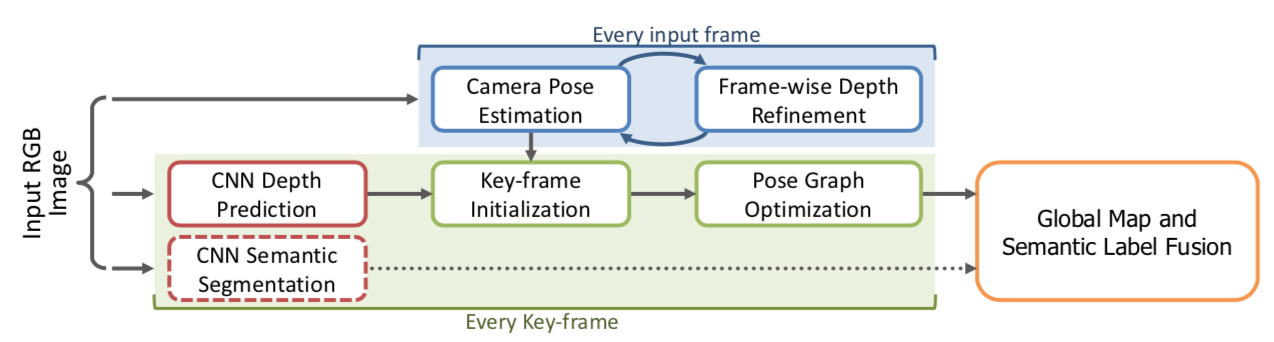
\includegraphics[width=.9\textwidth]{cnn-architecture}
      \captionsetup{labelformat=empty}
      \caption{Малюнак \cursection.\arabic{figure}: архітэктура CNN-SLAM}
      \label{fig:cnn-architecture}
    \end{figure}

    \item дадатковая нейронная сетка для семантычнай сегментацыі выяваў -- асобнае даследаванне,
    праведзенае ў межах працы і рэалізаванае ў тым жа фрэймворку;
    \item вынікі эксперыментаў паказваюць, што алгарытм на большасці набораў дадзеных працуе
    хутчэй за LSD-SLAM і ORB-SLAM, сённяшніх лідэраў сярод SLAM-алгарытмаў,
    з якімі праводзілася параўнанне, а таксама дае непараўнальна лепшую ацэнку для глыбіні сцэны;
    \item апроч таго, былі праведзеныя асобныя эксперыменты па прымяняльнасці алгарытма да
    дадзеных, якія атрымліваліся толькі праз павароты камеры. Паколькі гэтая папулярная сярод
    SLAM-сістэмаў праблема ў выпадку з CNN-SLAM абыходзіцца праз выкарыстанне нейронных сетак
    для ацэнкі глыбіні, то, як вынік, алгарытм паказвае дастойныя вынікі на такога кшталту дадзеных
    і моцна апярэджвае любыя іншыя сучасныя алгарытмы;
    \item архітэктура сістэмы прадстаўленая на малюнку \cursection.\ref{fig:cnn-architecture}.
\end{itemize}

\newpage

\begin{center}
    \addcontentsline{toc}{section}{ПРАКТЫЧНАЯ РЭАЛІЗАЦЫЯ}
    \section*{ГЛАВА 2. \\ ПРАКТЫЧНАЯ РЭАЛІЗАЦЫЯ}
\end{center}

\renewcommand{\floatpagefraction}{.8}%

У гэтым раздзеле я хачу апісаць дзве практычныя часткі, зробленыя мной.
Першая - серыя эксперыментаў над выманнем асаблівых кропак, падлікам іх дэскрыптараў і
пошукам адпаведнасцяў паміж дзвюма выявамі з аднаго набору.
Другая - апісанне распрацаванага праграмнага забеспячэння, якое выконвае ўвесь цыкл рэканструкцыі,
пабудаванае на аснове бібліятэкі \cite{theia-sfm}.

\vspace{5mm}

\addcontentsline{toc}{subsection}{Эксперыменты над асаблівасцямі выяваў}
\subsection*{2.1 Эксперыменты над спосабамі вымання асаблівых кропак, іх апісання і пошуку}

Практычна-даследніцкая частка маёй працы - параўнанне розных дэтэктараў, дэскрыптараў, тыпаў ключавых кропак
на рознага кшталту дадзеных, пошук узаемасувязі паміж тыпам пачатковых дадзеных і якасцю вынікаў, у залежнасці
ад прымененых алгарытмаў.

\vspace{5mm}

Для правядзення эксперыментаў я выбраў 4 набора дадзеных па 2 выявы. Крытэрам выбара была разнастайнасць: выявы павінны быць моцна альбо
слаба тэкстураванымі; адрознівацца паваротам, паралельным пераносам альбо выбарам іншага вугла камеры і г.д., яскравайвыраджанай
альбо аднастайнай каляровай гамай. Далей ідзе кароткае апісанне кожнага з набораў.

\begin{itemize}
    \item \textit{church:} два фотаздымкі царквы ў Швейцарыі, зробленыя з БПЛА.
    Маюць яскравую выраджанасць асобных аб'ектаў, у першую чаргу будынкаў. Гл. малюнкі \ref{fig:church}.
    \item \textit{fountain:} два фотаздымкі фантана, зробленыя пад розным вуглом.
    Пераважвае адзіная каляровая гамма, выявы слаба тэкстураваныя. Гл. малюнак \ref{fig:fountain}.
    \item \textit{ellis:} два фотаздымкі з выглядам на Манхэтэн, прыблізна палову
    кожнага здымка займае аднастайныя тэкстуры: вада, дарога. Аб'екты, якія знаходзяцца
    на абодвух выявах, моцна адрозніваюцца масштабам. Гл. малюнак \ref{fig:ellis}.
    \item \textit{grass:} два фотаздымкі беларускай сельскай мясцовасці зробленыя з БПЛА.
    Большая частка абодвух выяваў занятыя аднастайнай, практычна алнакаляровай тэкстурай. Гл. малюнак \ref{fig:grass}
\end{itemize}

Усе выявы былі папярэдне прыведзеныя да параўнальных памераў: вышыня кожнай выявы склала 640 пікселяў,
шырыня вылічвалася з захаваннем прапорцыяў.

Усе эксперыменты праводзіліся пры аднолькавых умовах, на камп'ютары з усталяванай ubuntu 16.04 з 2gb RAM на аднаядравым працэсары.
Рэалізацыі алгарытмаў браліся з бібліятэкі камп'ютарнага зроку з адкрытым зыходным кодам OpenCV.

Для кожнага набора дадзеных падлікі прадстаўленыя ў дзвюх табліцах.
У першай табліцы ідзе апісанне часавых характарыстыкаў дэтэкцыі кропак і падліку іх апісання рознымі алгарытмамі.
У другой - часавыя і колькасныя характарыстыкі алгарытмаў пошуку адпаведнасцяў паміж дзвюма выявамі з набора.

Вынікі эксперыментаў для дадзеных \textit{church} прыведзеныя ў табліцах \ref{table:church-kp} i \ref{table:church-matching},
\textit{fountain} - \ref{table:fountain-kp} i \ref{table:fountain-matching},
\textit{ellis} - \ref{table:ellis-kp} i \ref{table:ellis-matching},
\textit{grass} - \ref{table:grass-kp} i \ref{table:grass-matching}. У кожнай табліцы час прыведзены ў секундах.

\begin{figure}[H]
\centering
\begin{subfigure}{.5\textwidth}
  \centering
  \includegraphics[width=.95\linewidth]{swiss-church0.jpg}
\end{subfigure}%
\begin{subfigure}{.5\textwidth}
  \centering
  \includegraphics[width=.95\linewidth]{swiss-church1.jpg}
\end{subfigure}
\captionsetup{labelformat=empty}
\caption{Малюнак \arabic{figure}: набор дадзеных church}
\label{fig:church}
\end{figure}

\begin{table}[h]
  \centering
  \begin{footnotesize}
  \begin{tabular}{ | p{16mm} | p{17mm} | p{19mm} | p{22mm} | p{20mm} | p{22mm} | p{22mm} | }
    \hline
    Тып дэтэктара & Сярэдняя колькасць кропак & Час дэтэкцыі & Час на адну ключавую кропку & Тып дэскрыптара & Час на падлік дэскрыптараў & Час на падлік аднаго дэскрыптара \\ \hline
    SIFT & 4109 & 0.3951 & 0.0000481 & SIFT & 0.6190 & 0.0000753 \\ \hline
    SURF & 5291 & 0.4141 & 0.0000391 & SURF & 1.3550 & 0.0001280 \\ \hline
    BRISK & 13478 & 0.3624 & 0.0000134 & BRISK & 0.2292 & 0.0000085 \\ \hline
    ORB & 3000 & 0.0359 & 0.0000060 & ORB & 0.0213 & 0.0000036 \\ \hline
    AKAZE & 3655 & 0.4810 & 0.0000658 & AKAZE & 0.4024 & 0.0000550 \\ \hline
    CenSurE & 1077 & 0.0240 & 0.0000111 & BRIEF & 0.0070 & 0.0000032 \\ \hline
  \end{tabular}
  \end{footnotesize}
\captionsetup{labelformat=empty,justification=centering}
\caption{Табліца \arabic{table}: пошук асаблівых кропак і падлік адпаведных дэскрыптараў на наборы \textit{church}}
\label{table:church-kp}
\end{table}

\begin{table}[h]
  \centering
  \begin{footnotesize}
  \begin{tabular}{ | p{20mm} | p{22mm} | p{15mm} | p{22mm} | p{15mm} | p{22mm} | p{15mm} | }
    \hline
    Дэтэктар, дэскрыптар & BF адпаведнасцяў & BF час & BF-knn адпаведнасцяў & BF-knn час & FLANN адпаведнасцяў & FLANN час \\ \hline
    SIFT & 2207 & 1.5363 & 83 & 1.5089 & 62 & 0.1324 \\ \hline
    SURF & 2438 & 1.1988 & 118 & 1.1760 & 67 & 0.1266 \\ \hline
    BRISK & 6569 & 6.9033 & 89 & 6.9348 & 45 & 1.0028 \\ \hline
    ORB & 1575 & 0.2020 & 22 & 0.1912 & 19 & 0.0474 \\ \hline
    AKAZE & 1936 & 0.4880 & 145 & 0.5027 & 93 & 0.2132 \\ \hline
    CenSurE+\newline BRIEF & 509 & 0.0230 & 38 & 0.0233 & 19 & 0.0100 \\ \hline
  \end{tabular}
  \end{footnotesize}
\captionsetup{labelformat=empty,justification=centering}
\caption{Табліца \arabic{table}: пошук адпаведнасцяў на наборы \textit{church}}
\label{table:church-matching}
\end{table}

\begin{figure}[H]
\centering
\begin{subfigure}{.5\textwidth}
  \centering
  \includegraphics[width=.95\linewidth]{fountain0.png}
\end{subfigure}%
\begin{subfigure}{.5\textwidth}
  \centering
  \includegraphics[width=.95\linewidth]{fountain1.png}
\end{subfigure}
\captionsetup{labelformat=empty}
\caption{Малюнак \arabic{figure}: набор дадзеных fountain}
\label{fig:fountain}
\end{figure}

\begin{table}[h]
  \centering
  \begin{footnotesize}
  \begin{tabular}{ | p{16mm} | p{17mm} | p{19mm} | p{22mm} | p{20mm} | p{22mm} | p{22mm} | }
    \hline
    Тып дэтэктара & Сярэдняя колькасць кропак & Час дэтэкцыі & Час на адну ключавую кропку & Тып дэскрыптара & Час на падлік дэскрыптараў & Час на падлік аднаго дэскрыптара \\ \hline
    SIFT & 2953 & 0.4213 & 0.0000713 & SIFT & 0.5333 & 0.0000903 \\ \hline
    SURF & 4703 & 0.4138 & 0.0000440 & SURF & 1.4973 & 0.0001592 \\ \hline
    BRISK & 2142 & 0.0583 & 0.0000136 & BRISK & 0.0387 & 0.0000090 \\ \hline
    ORB & 2907 & 0.0299 & 0.0000051 & ORB & 0.0248 & 0.0000043 \\ \hline
    AKAZE & 776 & 0.3693 & 0.0002378 & AKAZE & 0.2518 & 0.0001622 \\ \hline
    CenSurE & 173 & 0.0316 & 0.0000913 & BRIEF & 0.0038 & 0.0000110 \\ \hline
  \end{tabular}
  \end{footnotesize}
\captionsetup{labelformat=empty,justification=centering}
\caption{Табліца \arabic{table}: пошук асаблівых кропак і падлік адпаведных дэскрыптараў на наборы \textit{fountain}}
\label{table:fountain-kp}
\end{table}

\begin{table}[h]
  \centering
  \begin{footnotesize}
  \begin{tabular}{ | p{20mm} | p{22mm} | p{15mm} | p{22mm} | p{15mm} | p{22mm} | p{15mm} | }
    \hline
    Дэтэктар, дэскрыптар & BF адпаведнасцяў & BF час & BF-knn адпаведнасцяў & BF-knn час & FLANN адпаведнасцяў & FLANN час \\ \hline
    SIFT & 1399 & 0.7398 & 68 & 0.7324 & 40 & 0.0827 \\ \hline
    SURF & 2082 & 0.9625 & 70 & 0.9743 & 44 & 0.1080 \\ \hline
    BRISK & 974 & 0.1673 & 28 & 0.1581 & 22 & 0.0365 \\ \hline
    ORB & 1446 & 0.2204 & 18 & 0.2039 & 11 & 0.0660 \\ \hline
    AKAZE & 338 & 0.0210 & 35 & 0.0213 & 25 & 0.0083 \\ \hline
    CenSurE+\newline BRIEF & 63 & 0.0008 & 14 & 0.0007 & 15 & 0.0009 \\ \hline
  \end{tabular}
  \end{footnotesize}
\captionsetup{labelformat=empty,justification=centering}
\caption{Табліца \arabic{table}: пошук адпаведнасцяў на наборы \textit{fountain}}
\label{table:fountain-matching}
\end{table}

\begin{figure}[H]
\centering
\begin{subfigure}{.5\textwidth}
  \centering
  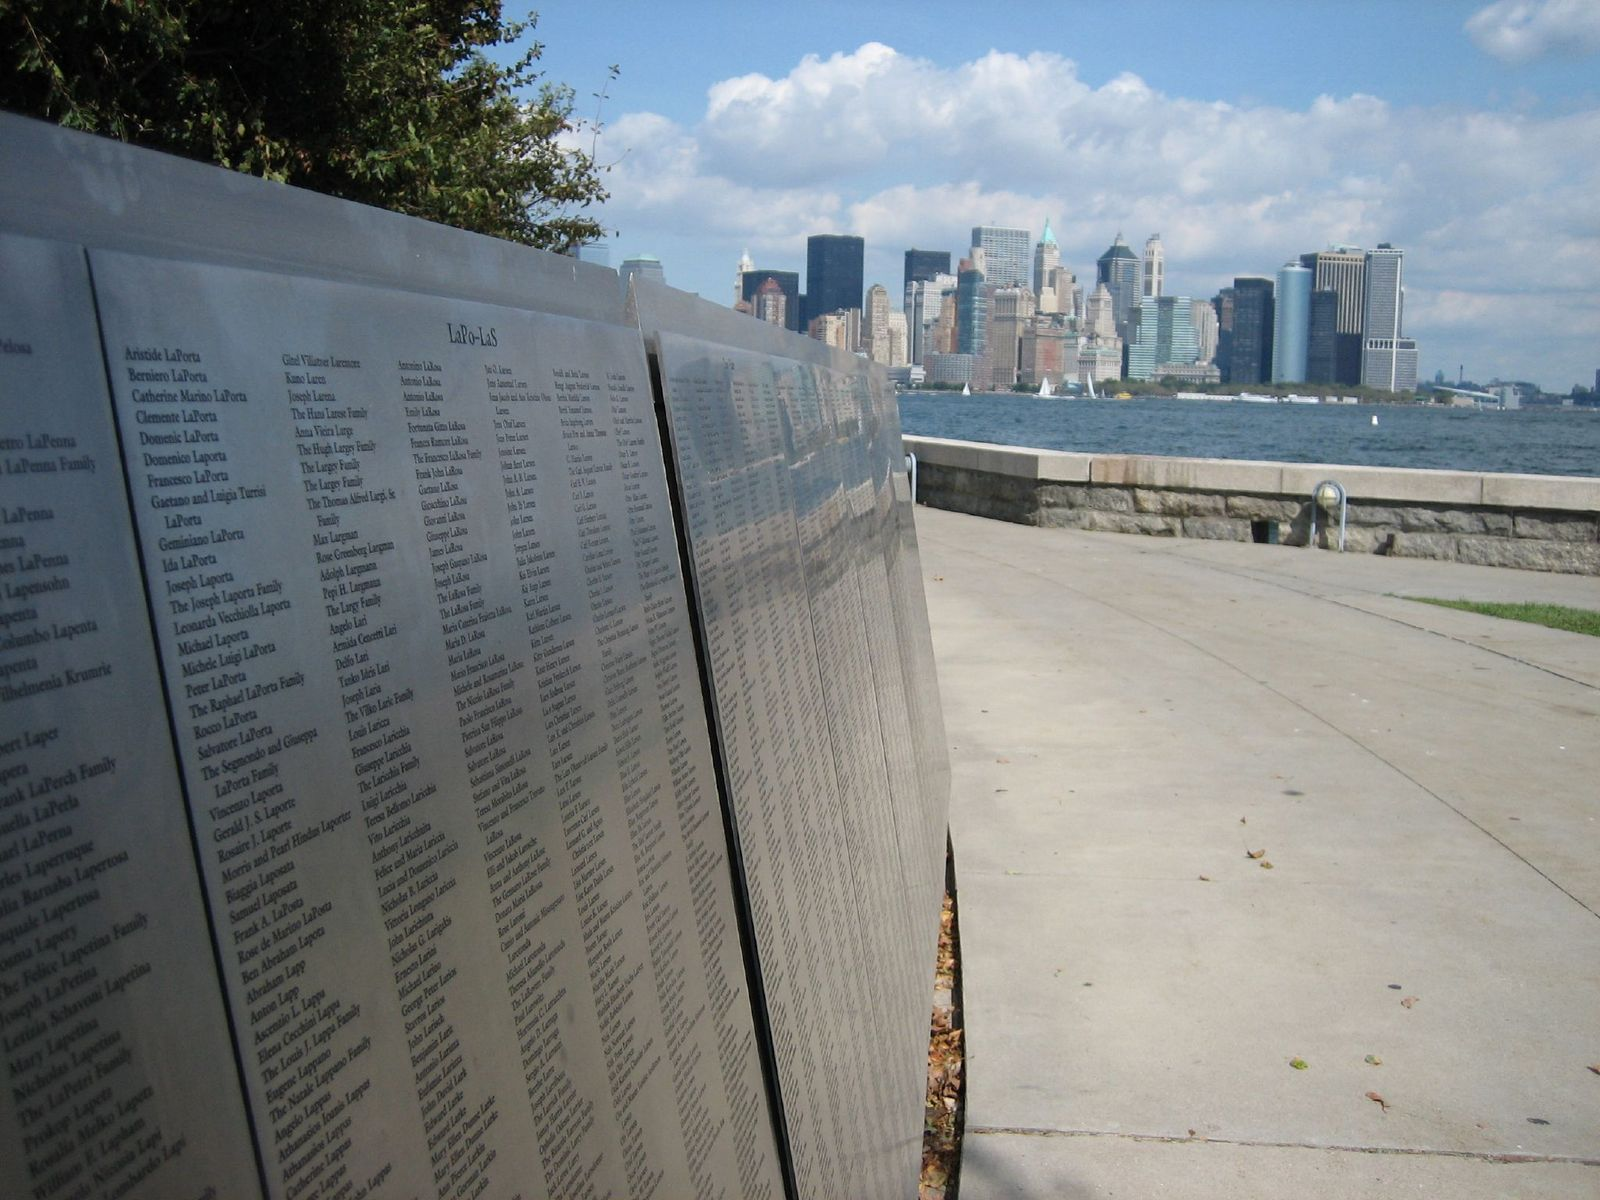
\includegraphics[width=.95\linewidth]{ellis0.jpg}
\end{subfigure}%
\begin{subfigure}{.5\textwidth}
  \centering
  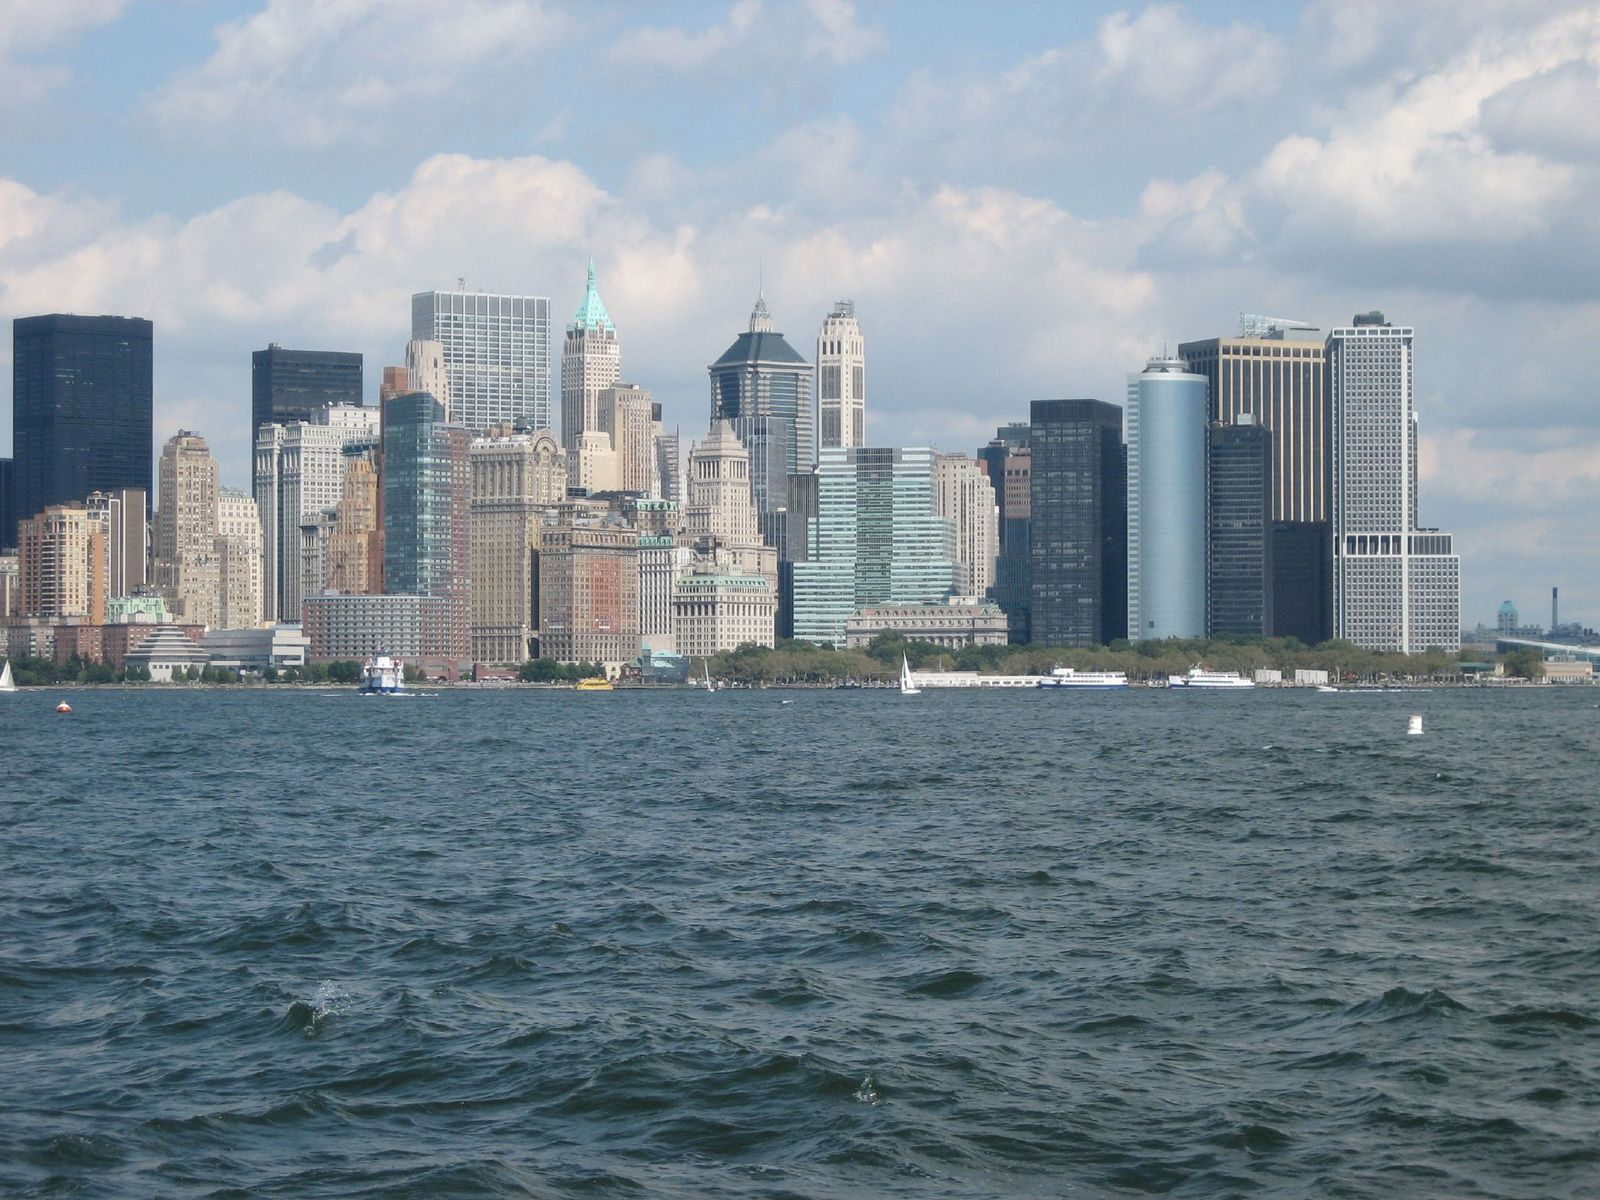
\includegraphics[width=.95\linewidth]{ellis1.jpg}
\end{subfigure}
\captionsetup{labelformat=empty}
\caption{Малюнак \arabic{figure}: набор дадзеных ellis}
\label{fig:ellis}
\end{figure}

\begin{table}[h]
  \centering
  \begin{footnotesize}
  \begin{tabular}{ | p{16mm} | p{17mm} | p{19mm} | p{22mm} | p{20mm} | p{22mm} | p{22mm} | }
    \hline
    Тып дэтэктара & Сярэдняя колькасць кропак & Час дэтэкцыі & Час на адну ключавую кропку & Тып дэскрыптара & Час на падлік дэскрыптараў & Час на падлік аднаго дэскрыптара \\ \hline
    SIFT & 2725 & 0.4967 & 0.0000911 & SIFT & 0.6985 & 0.0001281 \\ \hline
    SURF & 4950 & 0.4373 & 0.0000442 & SURF & 1.3399 & 0.0001353 \\ \hline
    BRISK & 3619 & 0.0883 & 0.0000122 & BRISK & 0.0716 & 0.0000099 \\ \hline
    ORB & 2947 & 0.0217 & 0.0000037 & ORB & 0.0240 & 0.0000041 \\ \hline
    AKAZE & 917 & 0.3723 & 0.0002029 & AKAZE & 0.2570 & 0.0001401 \\ \hline
    CenSurE & 261 & 0.0311 & 0.0000597 & BRIEF & 0.0023 & 0.0000044 \\ \hline
  \end{tabular}
  \end{footnotesize}
\captionsetup{labelformat=empty,justification=centering}
\caption{Табліца \arabic{table}: пошук асаблівых кропак і падлік адпаведных дэскрыптараў на наборы \textit{ellis}}
\label{table:ellis-kp}
\end{table}

\begin{table}[h]
  \centering
  \begin{footnotesize}
  \begin{tabular}{ | p{20mm} | p{22mm} | p{15mm} | p{22mm} | p{15mm} | p{22mm} | p{15mm} | }
    \hline
    Дэтэктар, дэскрыптар & BF адпаведнасцяў & BF час & BF-knn адпаведнасцяў & BF-knn час & FLANN адпаведнасцяў & FLANN час \\ \hline
    SIFT & 1265 & 0.8107 & 158 & 0.6754 & 142 & 0.0785 \\ \hline
    SURF & 1746 & 1.0627 & 149 & 1.0799 & 118 & 0.1052 \\ \hline
    BRISK & 1796 & 0.6418 & 93 & 0.6134 & 78 & 0.1154 \\ \hline
    ORB & 1469 & 0.1894 & 111 & 0.2477 & 92 & 0.0463 \\ \hline
    AKAZE & 494 & 0.0343 & 76 & 0.0368 & 58 & 0.0142 \\ \hline
    CenSurE+\newline BRIEF & 126 & 0.0017 & 9 & 0.0020 & 11 & 0.0015 \\ \hline
  \end{tabular}
  \end{footnotesize}
\captionsetup{labelformat=empty,justification=centering}
\caption{Табліца \arabic{table}: пошук адпаведнасцяў на наборы \textit{ellis}}
\label{table:ellis-matching}
\end{table}

\begin{figure}[H]
\centering
\begin{subfigure}{.5\textwidth}
  \centering
  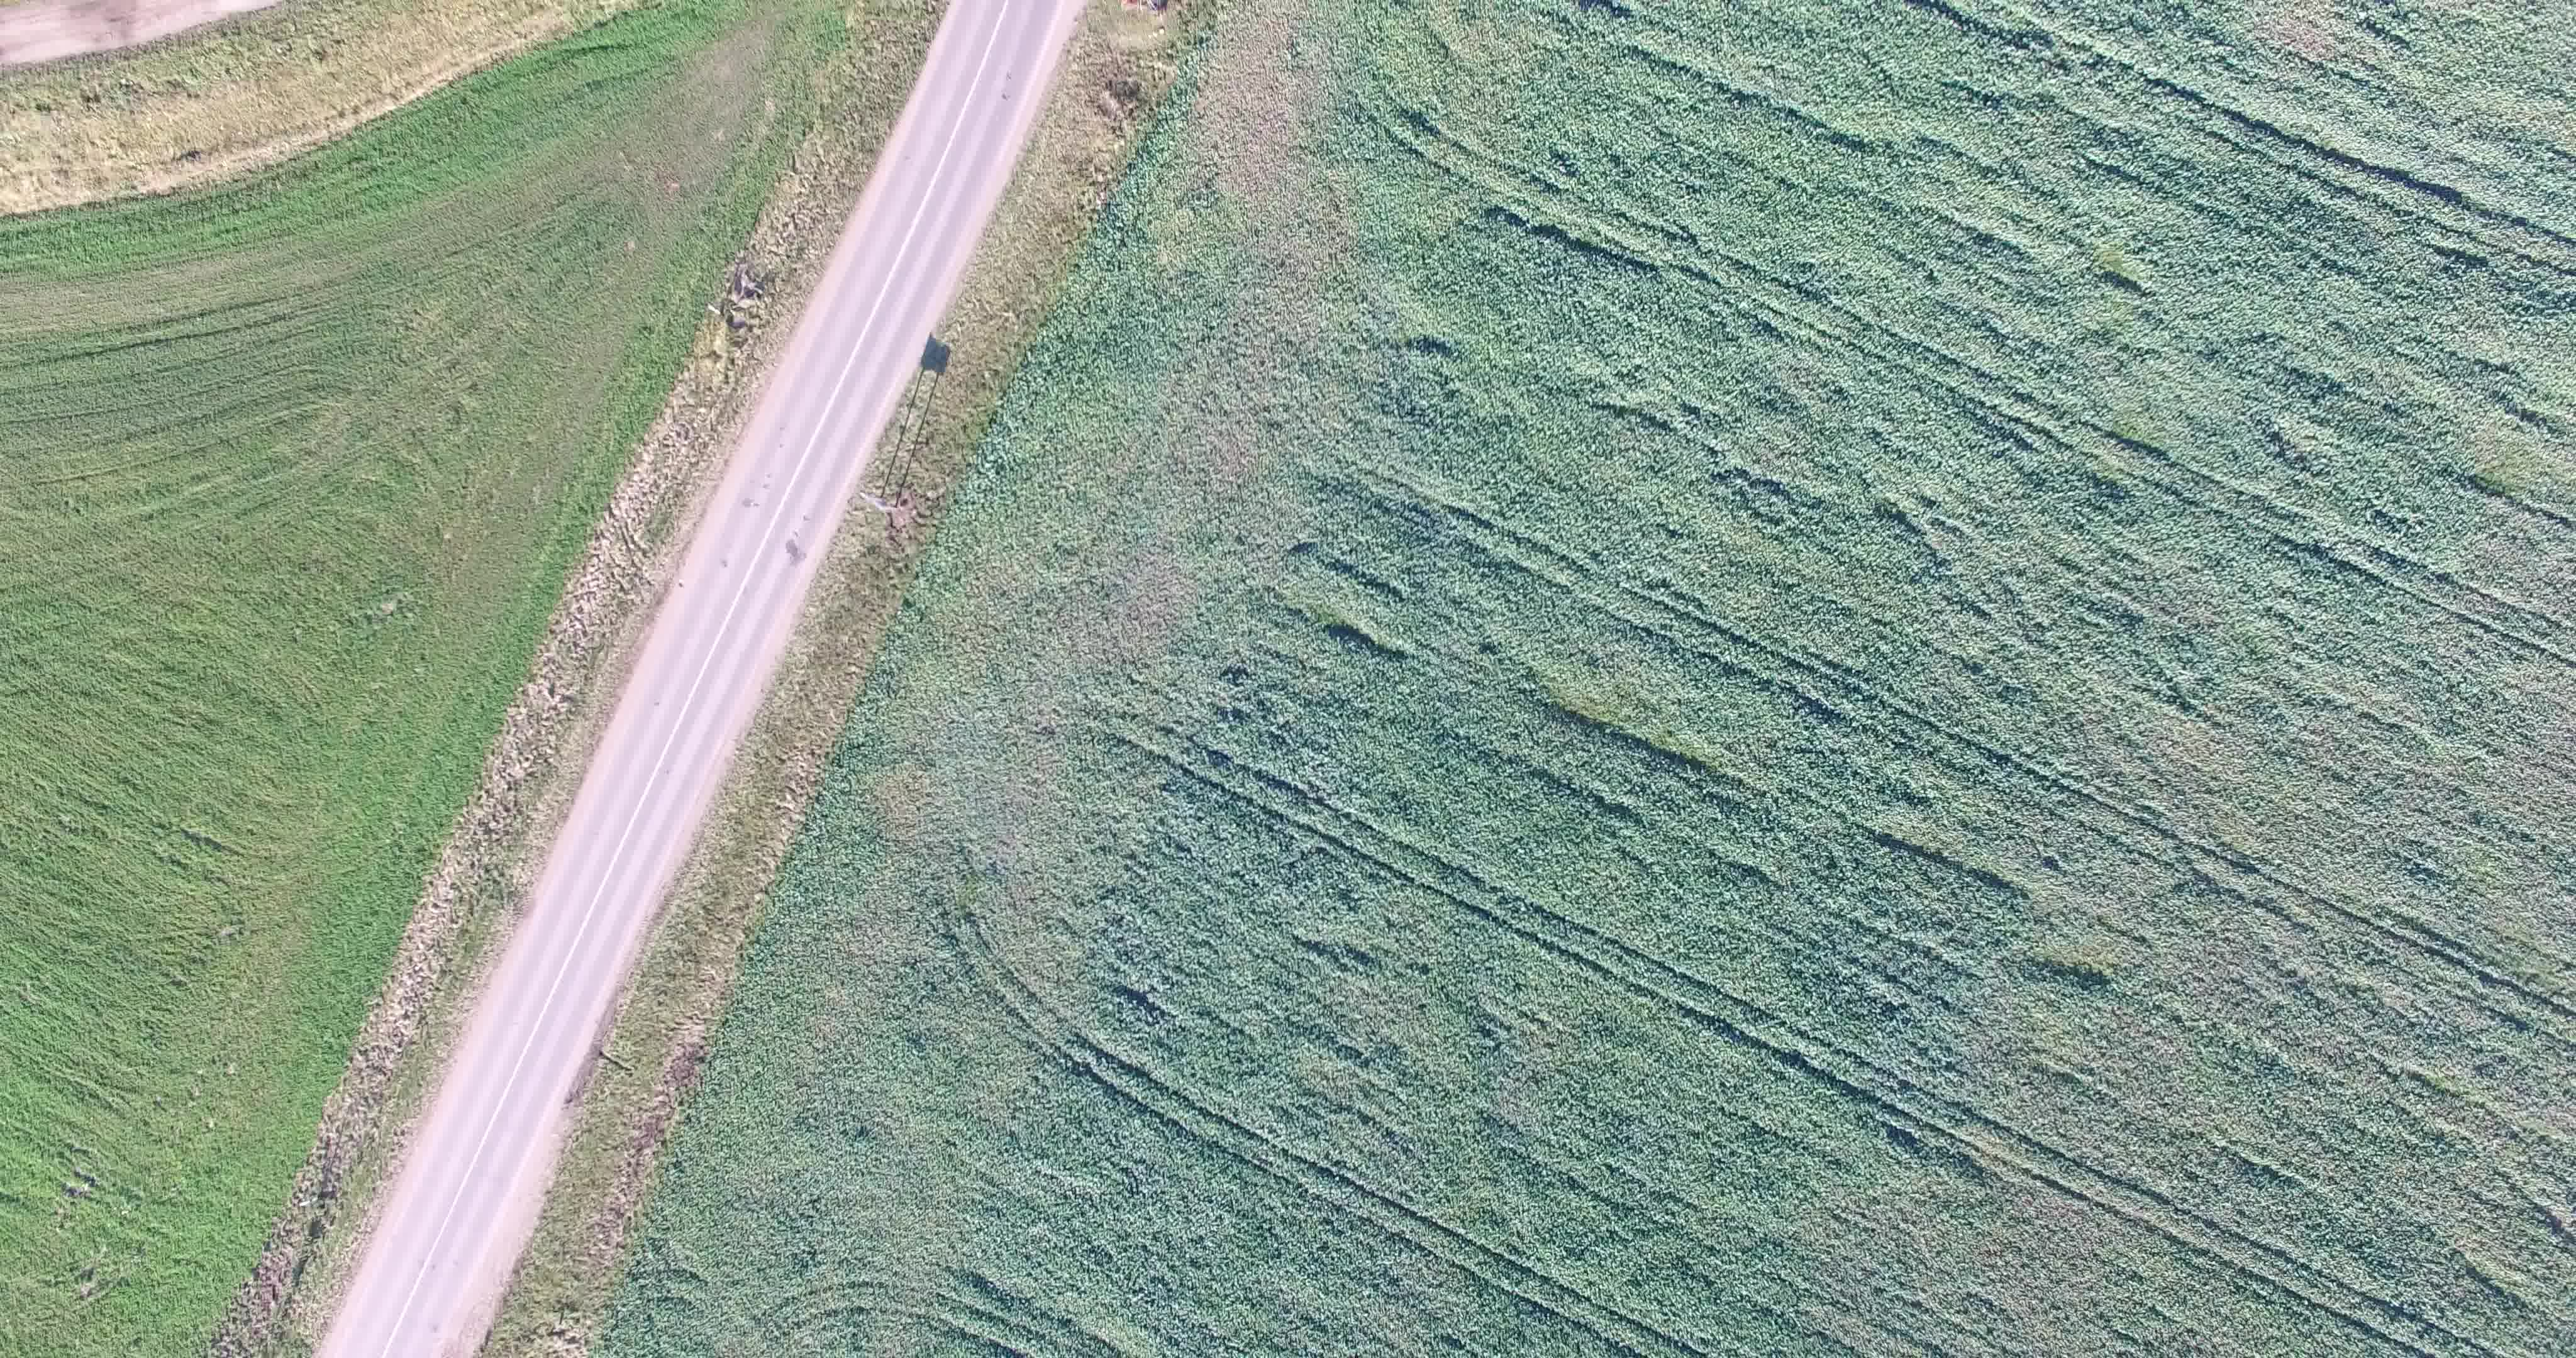
\includegraphics[width=.95\linewidth]{grass0.jpg}
\end{subfigure}%
\begin{subfigure}{.5\textwidth}
  \centering
  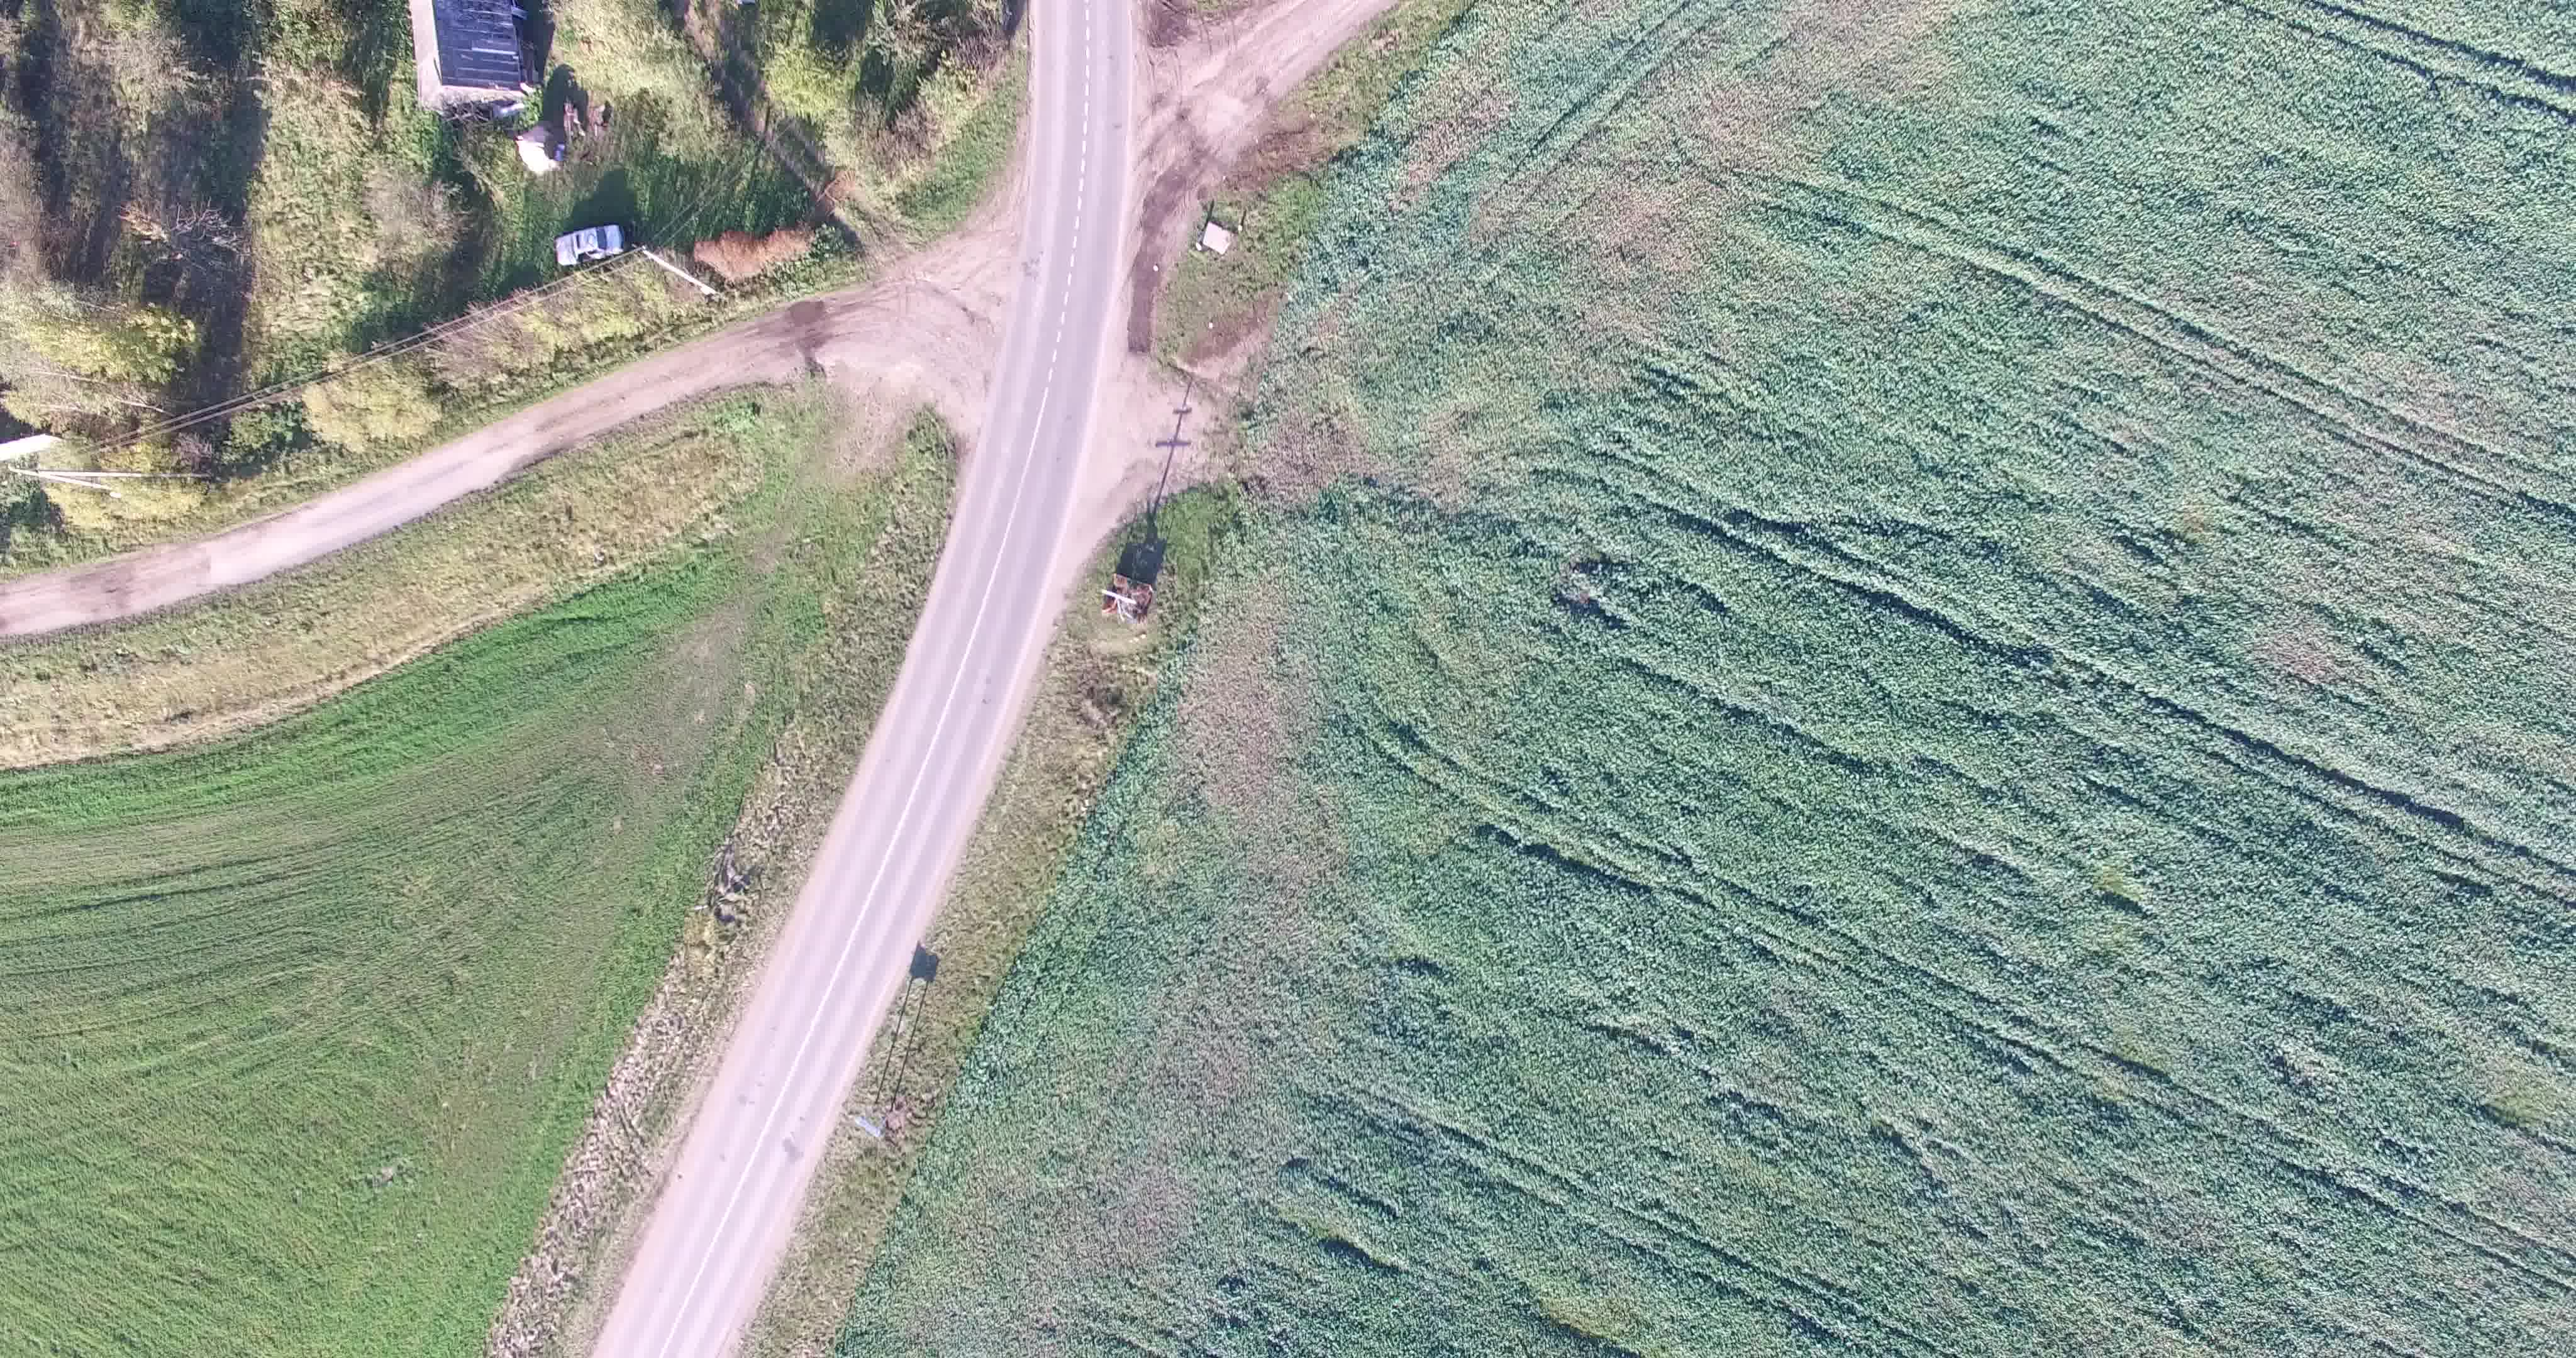
\includegraphics[width=.95\linewidth]{grass1.jpg}
\end{subfigure}
\captionsetup{labelformat=empty}
\caption{Малюнак \arabic{figure}: набор дадзеных grass}
\label{fig:grass}
\end{figure}

\begin{table}[h]
  \centering
  \begin{footnotesize}
  \begin{tabular}{ | p{16mm} | p{17mm} | p{19mm} | p{22mm} | p{20mm} | p{22mm} | p{22mm} | }
    \hline
    Тып дэтэктара & Сярэдняя колькасць кропак & Час дэтэкцыі & Час на адну ключавую кропку & Тып дэскрыптара & Час на падлік дэскрыптараў & Час на падлік аднаго дэскрыптара \\ \hline
    SIFT & 5357 & 0.6637 & 0.0000619 & SIFT & 0.9163 & 0.0000855 \\ \hline
    SURF & 15894 & 1.1313 & 0.0000356 & SURF & 3.5399 & 0.0001114 \\ \hline
    BRISK & 46305 & 1.3892 & 0.0000150 & BRISK & 0.8116 & 0.0000088 \\ \hline
    ORB & 3000 & 0.0921 & 0.0000154 & ORB & 0.0313 & 0.0000052 \\ \hline
    AKAZE & 3057 & 0.6880 & 0.0001125 & AKAZE & 0.7078 & 0.0001158 \\ \hline
    CenSurE & 829 & 0.1565 & 0.0000944 & BRIEF & 0.0199 & 0.0000120 \\ \hline
  \end{tabular}
  \end{footnotesize}
\captionsetup{labelformat=empty,justification=centering}
\caption{Табліца \arabic{table}: пошук асаблівых кропак і падлік адпаведных дэскрыптараў на наборы \textit{grass}}
\label{table:grass-kp}
\end{table}

\begin{table}[h]
  \centering
  \begin{footnotesize}
  \begin{tabular}{ | p{20mm} | p{22mm} | p{15mm} | p{22mm} | p{15mm} | p{22mm} | p{15mm} | }
    \hline
    Дэтэктар, дэскрыптар & BF адпаведнасцяў & BF час & BF-knn адпаведнасцяў & BF-knn час & FLANN адпаведнасцяў & FLANN час \\ \hline
    SIFT & 3043 & 2.6474 & 520 & 2.5827 & 452 & 0.1635 \\ \hline
    SURF & 8704 & 11.6172 & 848 & 11.5856 & 712 & 0.4455 \\ \hline
    BRISK & 24512 & 93.8451 & 1852 & 94.3301 & 1460 & 9.8551 \\ \hline
    ORB & 1624 & 0.2333 & 238 & 0.4267 & 207 & 0.1301 \\ \hline
    AKAZE & 1735 & 0.4762 & 732 & 0.4167 & 668 & 0.4133 \\ \hline
    CenSurE+\newline BRIEF & 452 & 0.0177 & 181 & 0.0188 & 172 & 0.0108 \\ \hline
  \end{tabular}
  \end{footnotesize}
\captionsetup{labelformat=empty,justification=centering}
\caption{Табліца \arabic{table}: пошук адпаведнасцяў на наборы \textit{grass}}
\label{table:grass-matching}
\end{table}

Кожны з набораў дадзеных апрацоўваўся шасцю рознымі алгарытмамі пошуку і падліку ключавых кропак.
Пры правядзенні эксперыменту была спроба прымянення і іншых алгарытмаў, якія не прысутнічаюць цяпер у табліцах,
аднак яны не паказалі вынікаў параўнальных з вышэй прыведзенымі. Напрыклад, натуральнай падавалася пара дэтэктар FAST і
дэскрыптар ORB, якая, аднак, паказала кепскія вынікі як па часе, так і па якасці знойдзеных адпаведнасцяў.

Прывядзем апісанне ўжытых метадаў пошука адпаведнасцяў згодна з іх скарачэннямі ў табліцах:
\begin{itemize}
  \item \textit{BF} - звычайны BruteForce алгарытм, рэалізацыя з OpenCV, запускаўся з параметрам \textit{CrossCheck = True}:
  гэты параметр кажа алгарытму вяртаць пару спалучаных дэскрыптараў толькі тады, калі кожны з дэскрыптараў на чарговым кроку
  выступае найлепшым для свайго адпаведніка на іншай выяве (то бок дэскрыптары павінны спалучацца ``у абодва бакі''). Гэта з'яўляецца
  своеасаблівай альтэрнатывай ``тэсту суадносінаў'' (англ. \textit{ratio test}),
  апісанаму ў \cite{sift-paper} - гэты тэст мы будзем запускаць разам з наступным метадам.
  \item \textit{BF-knn} - BruteForce алгарытм, які структуруе знойдзеныя адпаведнасці крыху іншым чынам, чым вышэйзгаданы BF:
  для кожнага дэскрыптара ён знаходзіць не больш за $k=2$ адпаведных дэскрытараў. Далей мы запускаем ``тэст суадносінаў'',
  які апісаны ў \cite{sift-paper} (старонка 20). Сцвярджаецца, што калі адлегласці двух найлепшых знойдзеных адпаведнікаў для
  вызначанага дэскрыптара адпавядаюць няроўнасці $distance_1 < ratio \times distance_2$, дзе $ratio$ - канстанта, якая звычайна
  абіраецца з прамежка $[0.7, 0.8]$, то першы адпаведнік для знойдзенага дэскрыптара з'яўляецца ``дастаткова добрым'' - такія дэскрыптары
  заносяцца ў табліцу як ``знойдзеныя''. Трэба заўважыць, што гэты ``тэст суадносінаў'' на практыцы праходзіць дастаткова мала
  параў дэскрыптараў.
  \item \textit{FLANN} - сямейства алгарытмаў набліжанага пошуку бліжэйшых суседзяў. У нашым выпадку, для SIFT i SURF гэты алгарытм
  заснаваны на KD-дрэвах, для астатніх дэскрыптараў гэта LSH (Locality-sensitive hashing).
\end{itemize}

Заўвагі:
\begin{itemize}
  \item алгарытм ORB прымае ў якасці аднаго з параметраў абмежаванне зверху на колькасць знойдзеных ключавых кропак;
  у табліцах \ref{table:church-kp} - \ref{table:grass-matching}, калі колькасць ключавых кропак, знойдзеных ORB, роўная 3000,
  гэта не азначае, што гэта максімальна магчымы лік; для астатніх алгарытмаў прыведзеныя максімальныя значэнні.
\end{itemize}

На малюнках \ref{fig:matches1} - \ref{fig:matches2} прыведзеныя два прыклады знойдзеных адпаведнасцяў. Колькасць нанесеных
у выглядзе лініяў адпаведнасцяў абмежаваная лікам 20 для паляпшэння нагляднасці.

\begin{figure}[H]
  \centering
  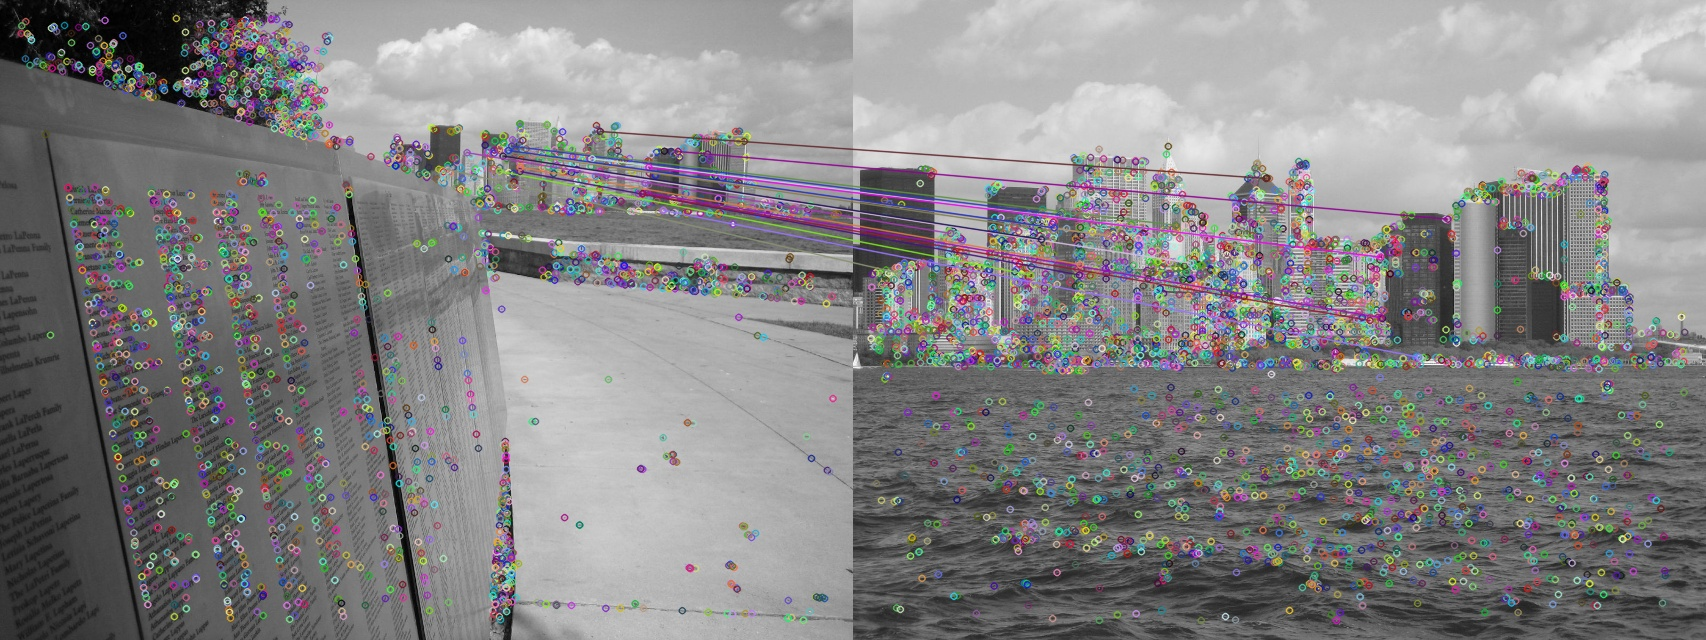
\includegraphics[width=.9\textwidth]{matches/ellis_BRISK_bf_crossCheck_matches.jpg}
  \captionsetup{labelformat=empty}
  \caption{Малюнак \arabic{figure}: знойдзеныя адпаведнасці (ellis, BRISK, BF)}
  \label{fig:matches1}
\end{figure}

\begin{figure}[H]
  \centering
  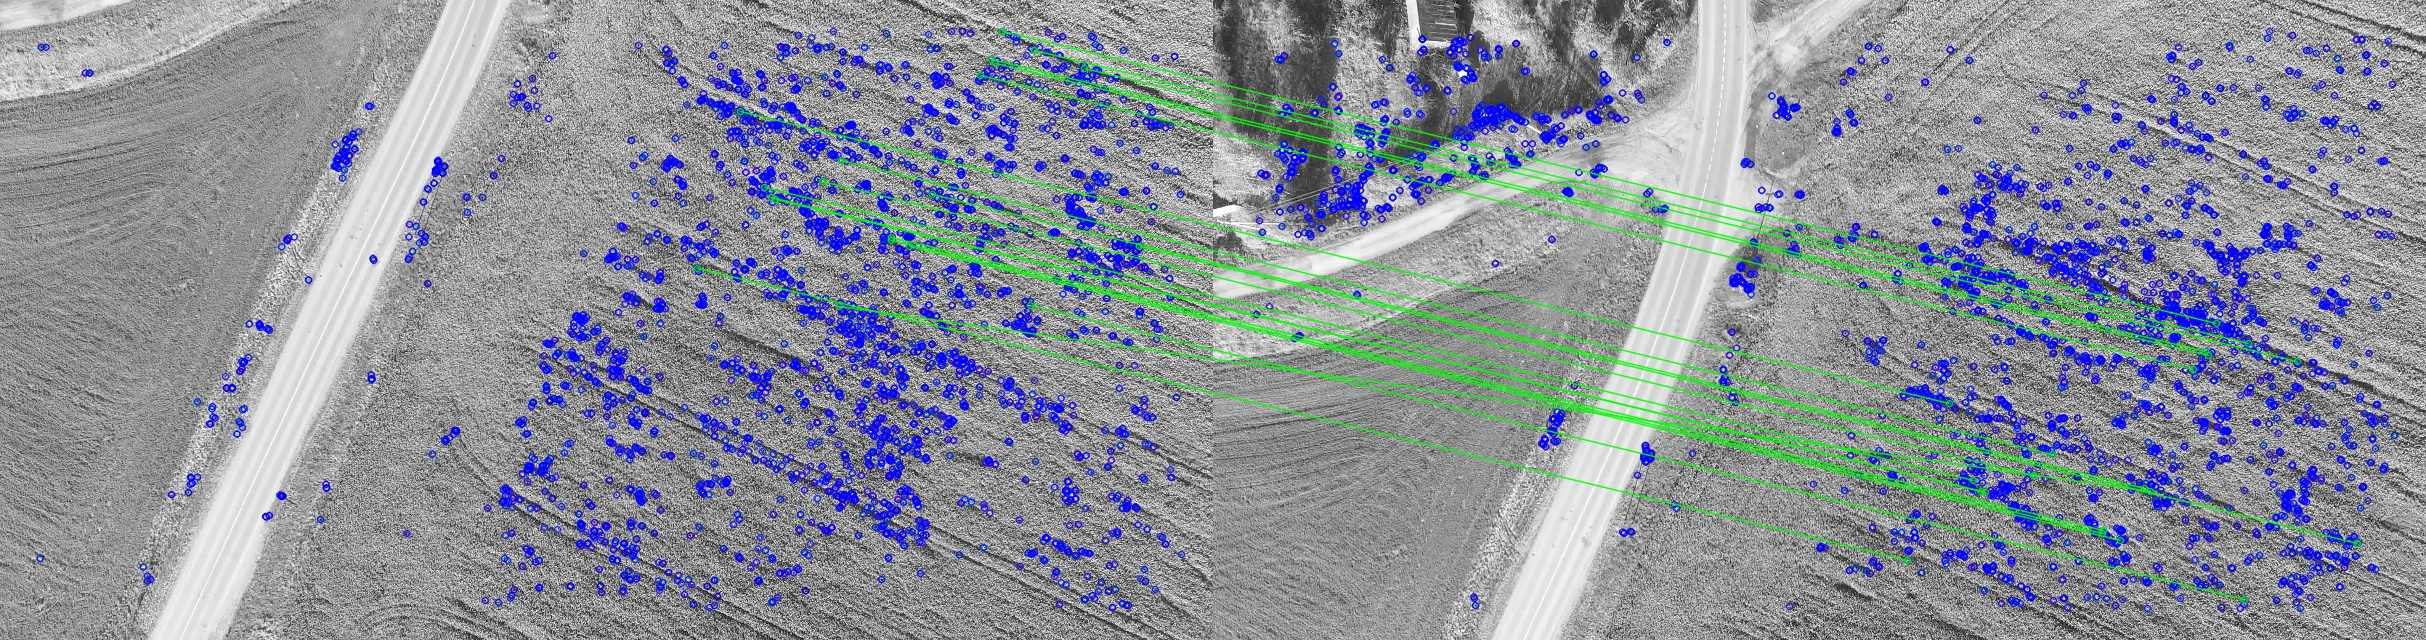
\includegraphics[width=.9\textwidth]{matches/grass_ORB_flann_knn_matches.jpg}
  \captionsetup{labelformat=empty}
  \caption{Малюнак \arabic{figure}: знойдзеныя адпаведнасці (grass, ORB, FLANN)}
  \label{fig:matches2}
\end{figure}

Высновы:
\begin{itemize}
  \item Алгарытмы дастаткова яскрава падзяліліся на ``хуткія'' і ``марудныя''. ORB заўсёды хутчэй за ўсіх знаходзіць
  ключавыя кропкі і падлічвае для іх дэскрыптары (часам гэтаму спрыяе штучнае абмежаванне ў 3000 на колькасць
  ключавых кропак). Пошук адпаведнасцяў таксама заўсёды адбываецца хутка (у параўнанні з іншым алгарытмамі),
  хаця і моцна вар'юецца: ад 0.02с да 0.4с.
  \item Пара алгарытмаў CenSurE+BRIEF знаходзіць малую колькасць ключавых кропак (часам на парадак менш, чым іншыя
  алгарытмы на тых жа наборах дадзеных), прычым па часе могуць прайграць таму ж ORB. Негледзячы на гэта, маленькая
  колькасць дазваляе вельмі хутка знаходзіць адпаведнасці.
  \item Алгарытм BRISK кепска прымяняецца да аднастайных дадзеных: на наборы \textit{grass} колькасць знойдзеных ключавых кропак
  рэзка ўзрастае (у ~3 разы больш за наступны па колькасці знойдзеных кропак алгарытм). На іншых наборах дадзеных BRISK
  паводзіць сябе зусім іншым чынам. У выніку алгарытм выкарыстаў рэкордны для нашага даследвання час на на пошук асаблівасцяў
  (~94c на BF i BF-knn). Трэба сказаць, што падобныя паводзіны за BRISK-ам былі заўважаныя і на іншых выявах
  са слабай тэкстураванасцю.
  \item У агульным выпадку можна казаць пра маруднасць алгарытма SURF на этапе падліку дэскрыптараў: на ўсіх чатырох
  наборах ён падлічваў значэнні дэскрыптараў з самым вялікім абсалютным значэннем па часе, і быў адным з самых
  марудных у пераліку на час на адзін дэскрыптар.
\end{itemize}

Агульнае падсумаванне можна сфармуляваць наступным чынам: існуюць алгарытмы для хуткай апрацоўкі і для больш грунтоўнай,
алгарытмы, якія паказваюць падобныя вынікі на любых дадзеных і алгарытмы, слаба прымяняльныя на канкрэтных дадзеных.
SIFT i SURF можна ўмоўна аднесці да надзейных, але марудных: яны часта выкарыстоўваюцца на прыладах з добрымі характарыстыкамі,
але радзей знаходзяць сваё прымяненне да мабільных прыладах. Нагадаем, што абодва гэтыя алгарытмы апісваюць ключавыя кропкі
пры дапамозе рэчаісных вектароў, што, вядома, марудней за бінарныя радкі.
Ва ўмовах абмежаваных рэсурсаў часта знаходзяць сваё прымяненне
алгарытмы ORB i AKAZE: у нашых лічбах яны з'яўляюцца найхутчэйшымі і найменш залежнымі ад рэсурсаў.
BRISK паводзіць сябе на ўзроўні іншых алгарытмаў (па колькасных і часавых характарыстыках), але на такіх наборах, як
\textit{church} альбо \textit{grass} паказвае рэзкае адставанне па часе на этапе пошуку адпаведнасцяў праз вялікую колькасць
папярэдне вылучаных асаблівых кропак.

Цікаўнасць для даследвання прадстаўляе таксама хуткасць роста ад дыстанцыі ў адсартаваных масівах знойдзеных адпаведнасцяў.
Дыстанцыя, па сутнасці, з'яўляецца непасрэднай характарыстыкай якасці знойдзенай адпаведнасці, а таксама проста ўплывае на тое,
ці пройдзе пара ``тэст суадносінаў'', які апісываўся вышэй.

На графіках \ref{fig:best20matches} - \ref{fig:best250matches} прадстаўленыя адлегласці лепшых адпаведна 20 і 250 параў дэскрыптараў.
Пары былі суаднесеныя BF алгарытмам. Дадзеныя на графіках палічаныя адносна апошняй (адпаведна, 20ай альбо 250ай) адлегласці.
Інтэрпрэтуюцца дадзеныя наступным чынам: рэзкі рост графіка абазначае рэзкі рост кожнай наступнай адлегласці, адпаведна - адлегласць
паміж кожнай наступнай парай дэскрыптараў значна больш. Разам з тым, больш спадзісты характар графіка сведчыць пра нізкі рост
у значэннях адлегласцяў. На графіках часцей за ўсё асобна выбіваецца AKAZE - у табліцах \ref{table:church-kp} - \ref{table:grass-matching}
гэта адлюстроўваецца ў тым, што на некаторых наборах дадзеных суадносіны ``колькасць адпаведнасцяў знойдзеных BF-knn да пачатковай
колькасці дэскрыптараў'' для AKAZE найвялікшая.

\begin{figure}[h]
\centering
\begin{subfigure}{.5\textwidth}
  \centering
  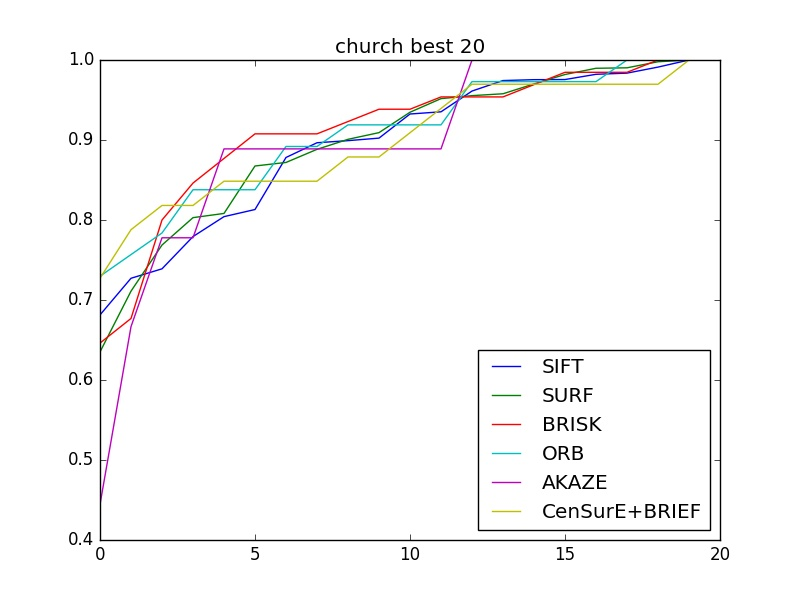
\includegraphics[width=\linewidth]{graphs/church_top20.jpg}
  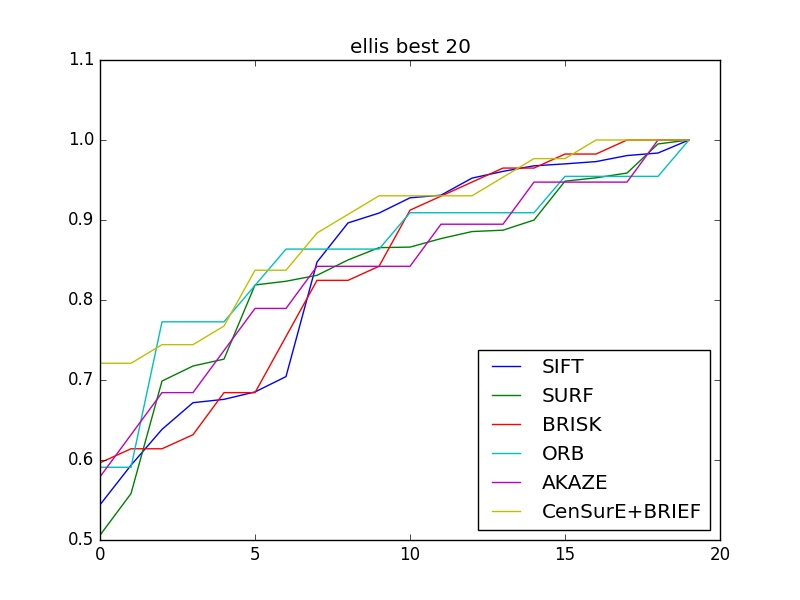
\includegraphics[width=\linewidth]{graphs/ellis_top20.jpg}
\end{subfigure}%
\begin{subfigure}{.5\textwidth}
  \centering
  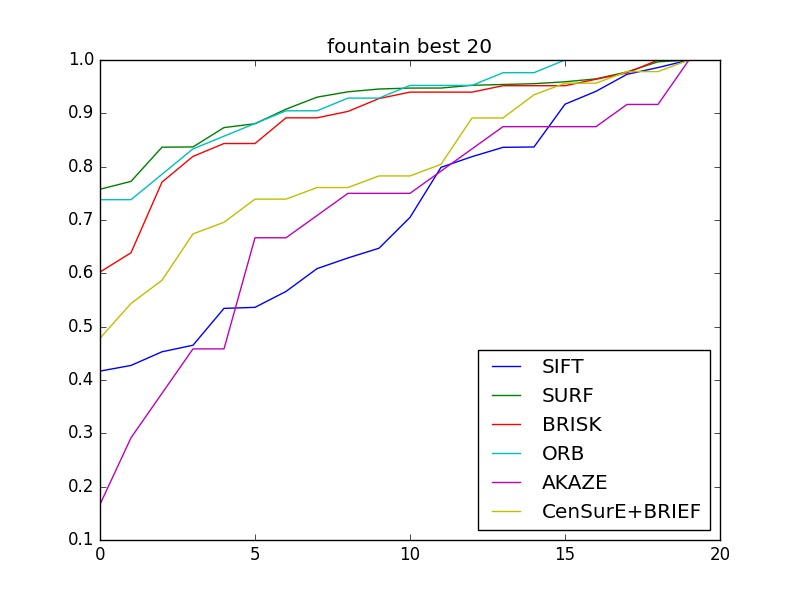
\includegraphics[width=\linewidth]{graphs/fountain_top20.jpg}
  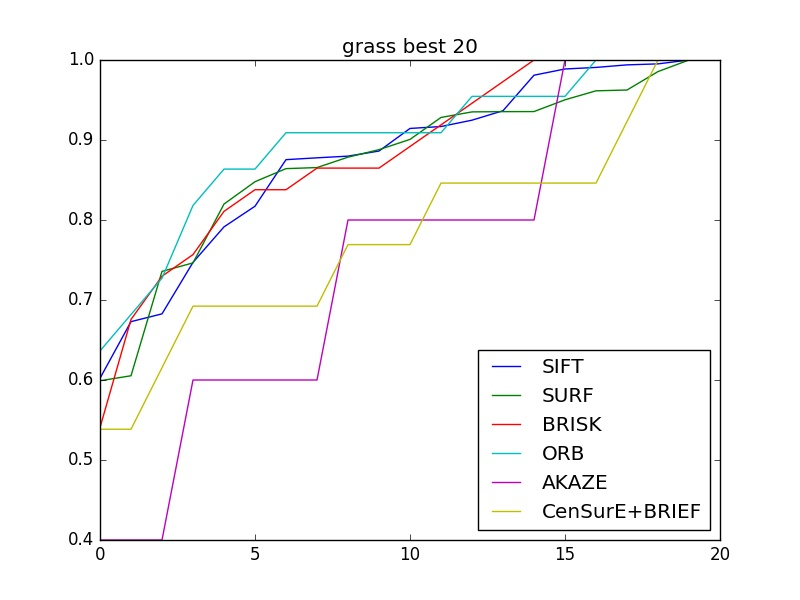
\includegraphics[width=\linewidth]{graphs/grass_top20.jpg}
\end{subfigure}%
\captionsetup{labelformat=empty,justification=centering}
\caption{Малюнак \arabic{figure}: рост адлегласці ў 20 лепшых парах}
\label{fig:best20matches}
\end{figure}

\begin{figure}[h]
\centering
\begin{subfigure}{.5\textwidth}
  \centering
  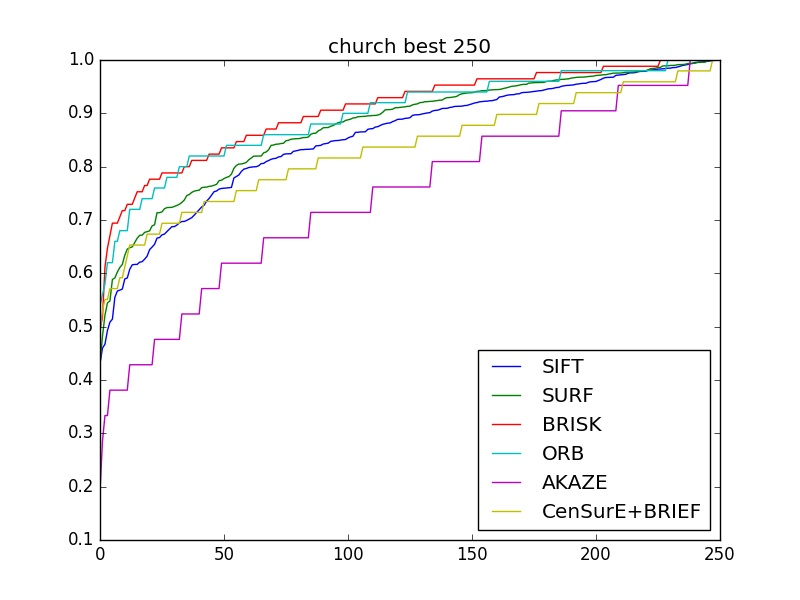
\includegraphics[width=\linewidth]{graphs/church_top250.jpg}
  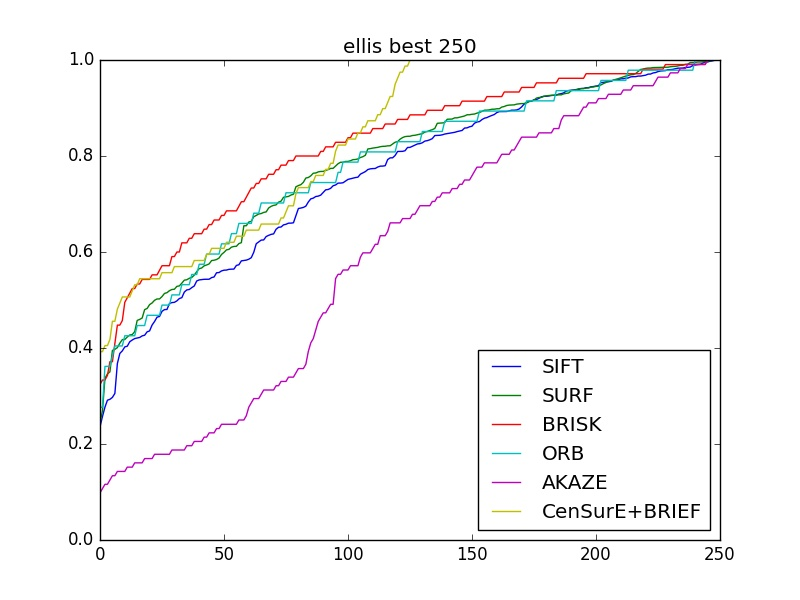
\includegraphics[width=\linewidth]{graphs/ellis_top250.jpg}
\end{subfigure}%
\begin{subfigure}{.5\textwidth}
  \centering
  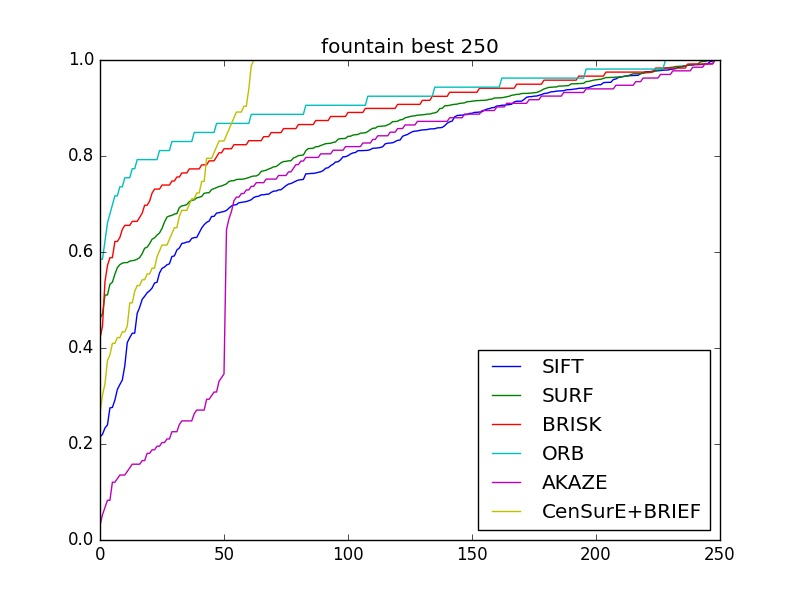
\includegraphics[width=\linewidth]{graphs/fountain_top250.jpg}
  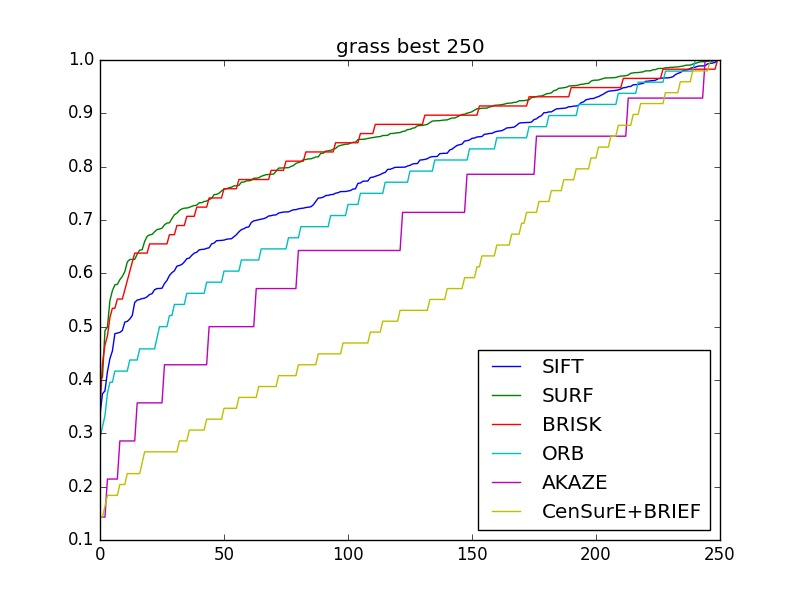
\includegraphics[width=\linewidth]{graphs/grass_top250.jpg}
\end{subfigure}%
\captionsetup{labelformat=empty,justification=centering}
\caption{Малюнак \arabic{figure}: рост адлегласці ў 250 лепшых парах}
\label{fig:best250matches}
\end{figure}

%
%
% APPA
%
%

\addcontentsline{toc}{subsection}{Распрацоўка праграмнага забеспячэння для рэканструкцыі паверхні}
\subsection*{2.2 Распрацоўка праграмнага забеспячэння для рэканструкцыі паверхні}

Асноўнай практычнай часткай маёй курсавой працы была рэалізацыя канечнай праграмы для рэканструкцыі паверхні па дадзеных
з БПЛА. Праграма напісаная на мове C++ з выкарыстаннем фрэймворка Qt на базе бібліятэкі камп'ютарнага зроку
з адкрытым зыходным кодам TheiaSfm \cite{theia-sfm}. Праграма
знаходзіцца ў актыўнай распрацоўцы, на дадзены момант рэалізаваныя ўсе асноўныя магчымасці, такія як адкрыццё/стварэнне новых праэктаў,
пабудова разрэджанага воблака кропак па наборы выяваў, трохмерная візуалізацыя мадэлі, падсветка выбранай камеры, паўторнае выкарыстанне
дадзеных (напрыклад, здзейсніўшы адзін раз пошук ключавых кропак, наступны раз гэты этап можа быць прапушчаны, што моцна эканоміць час
і рэсурсы), генерацыя справаздачаў пасля рэканструкцыі. Праграма працуе як у кансольным рэжыме, так і ў рэжыме з графічным
інтэрфейсам.

Праграма ствараецца з практычнымі метадамі: яна будзе карысная як для пабудовы мадэлі канечным карыстачом (выкарыстоўваючы
графічны інтэрфейс), так і, напрыклад, для правядзення эксперыментаў з алгарытмамі (у гэтым выпадку карыснай будзе магчымасць
выклікаць увесь функцыянал праграмы з кансольнага радка).

Праграма кросплатформенная, праца ўсяго функцыяналу была пратэставаная на аперацыйных сістэмах macOS i Ubuntu.

Здымкі экрана з запушчаным прыкладаннем прадстаўленыя на малюнках \ref{fig:screenshot1} - \ref{fig:screenshot3}.

\begin{figure}[H]
  \centering
  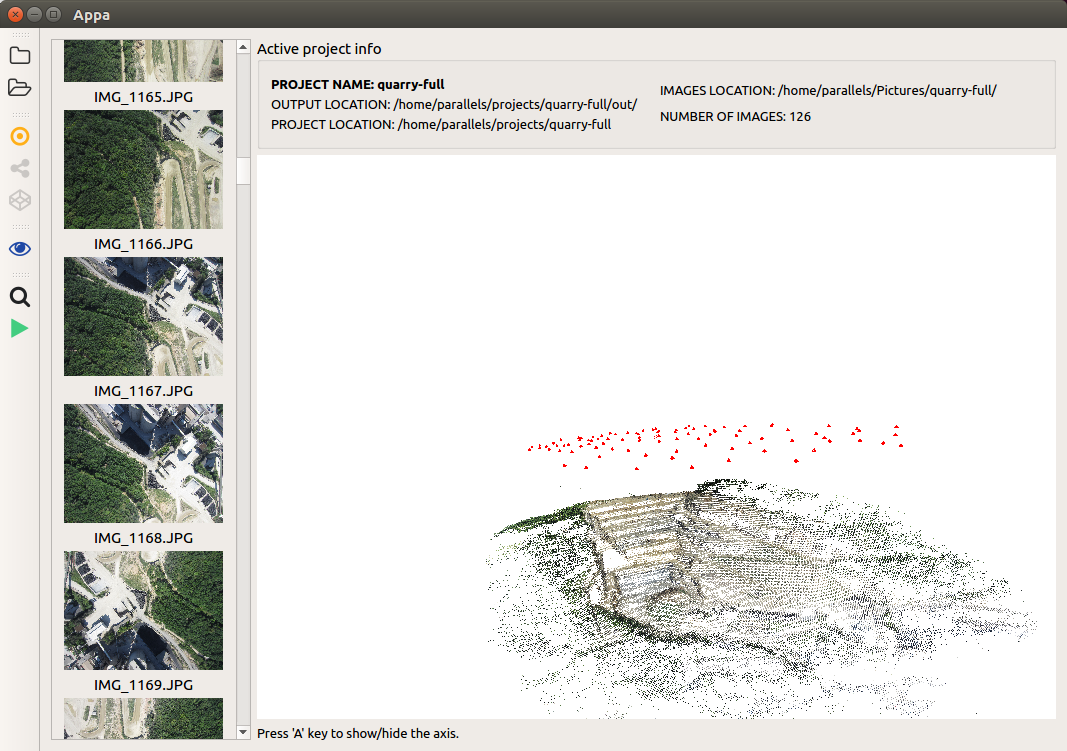
\includegraphics[width=.9\textwidth]{appa0.png}
  \captionsetup{labelformat=empty}
  \caption{Малюнак \arabic{figure}: здымак экрана}
  \label{fig:screenshot1}
\end{figure}

\begin{figure}[H]
  \centering
  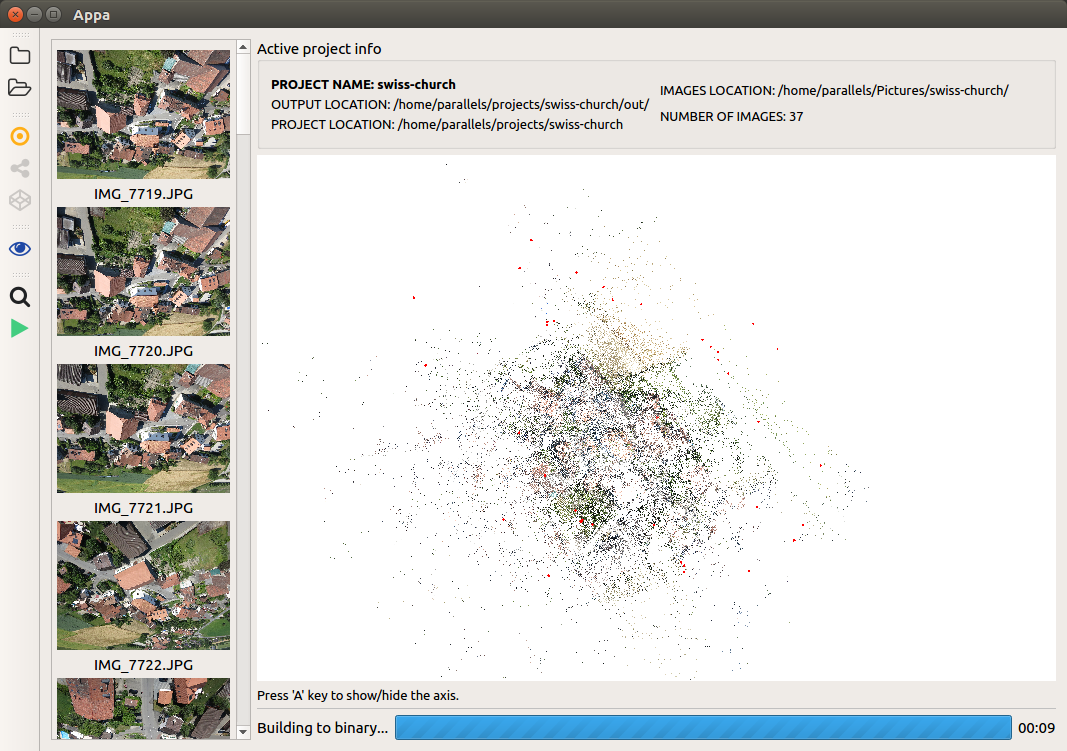
\includegraphics[width=.9\textwidth]{appa1.png}
  \captionsetup{labelformat=empty}
  \caption{Малюнак \arabic{figure}: здымак экрана}
  \label{fig:screenshot2}
\end{figure}

\begin{figure}[H]
  \centering
  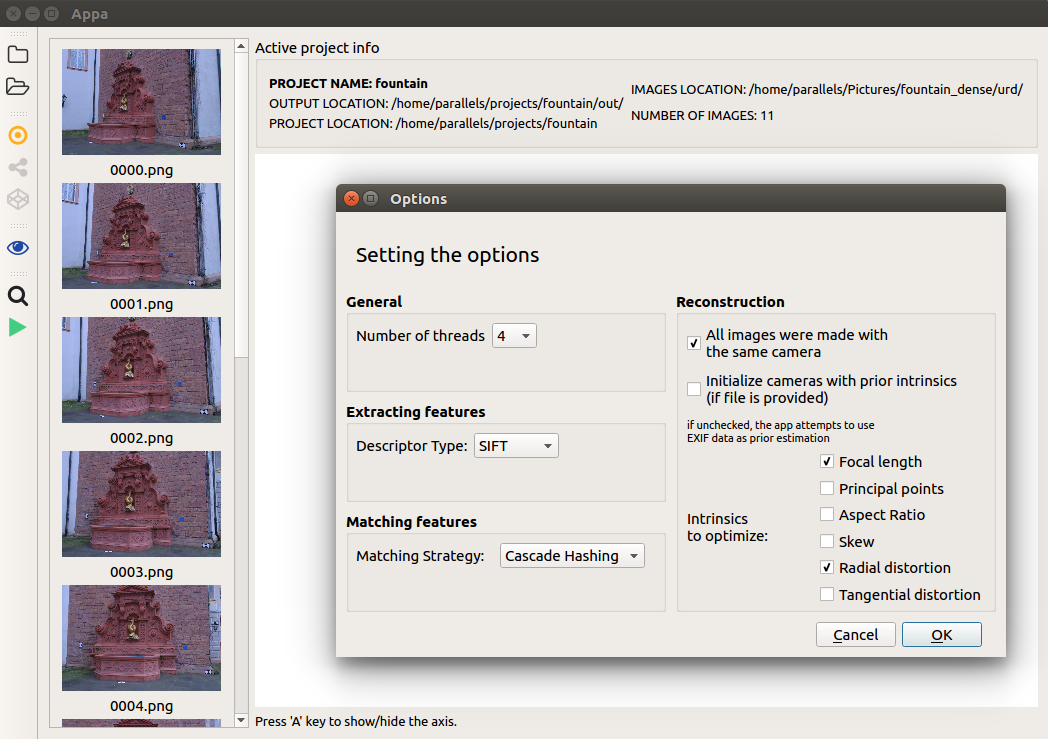
\includegraphics[width=.9\textwidth]{appa2.png}
  \captionsetup{labelformat=empty}
  \caption{Малюнак \arabic{figure}: здымак экрана}
  \label{fig:screenshot3}
\end{figure}

Увесь зыходны код адкрыты і размешчаны на GitHub.

\newpage


\section*{Высновы}

\subsection*{Ураўненне}

Для задачы Кашы \eqref{eq:my-equation} вядомае дакладнае рашэнне:
\begin{equation}
    u(x) = sin(x) - 1
\end{equation}
Таму мы маем магчымасць пабудаваць дакладную сетку значэнняў і параўнаць гэтыя значэнні з вынікамі працы кожнага з алгарытмаў.

{\small
\begin{verbatim}
Exact solution:
y(0.0) = -1.0
y(0.1) = -0.900166583353
y(0.2) = -0.801330669205
y(0.3) = -0.704479793339
y(0.4) = -0.610581657691
y(0.5) = -0.520574461396
y(0.6) = -0.435357526605
y(0.7) = -0.355782312762
y(0.8) = -0.2826439091
y(0.9) = -0.216673090373
y(1.0) = -0.158529015192
\end{verbatim}
}

Знойдзем хібнасці кожнага з метадаў, то бок для кожнага $x_i$ з сеткі знойдзем розніцу $u_i - y_i = u(x_i) - y(x_i)$, дзе $u_i$ - дакладнае значэнне, $y_i$ - набліжэнне.\par
\vspace{5mm}
Метад шэрагаў:
{\small
\begin{verbatim}
Series method
u(0.0) - y(0.0) = 0.0
u(0.1) - y(0.1) = 8.33134948808e-08
u(0.2) - y(0.2) = 5.74204981008e-07
u(0.3) - y(0.3) = 1.43037073175e-06
u(0.4) - y(0.4) = 2.6126972027e-06
u(0.5) - y(0.5) = 4.08658620521e-06
u(0.6) - y(0.6) = 5.82281987083e-06
u(0.7) - y(0.7) = 7.798065847e-06
u(0.8) - y(0.8) = 9.99512268285e-06
u(0.9) - y(0.9) = 1.24029964328e-05
u(1.0) - y(1.0) = 1.50168860044e-05
\end{verbatim}
}

Яўны метад Эйлера:
{\small
\begin{verbatim}
Explicit Euler:
u(0.0) - y(0.0) = 0.0
u(0.1) - y(0.1) = -0.000166583353172
u(0.2) - y(0.2) = -0.000814510619714
u(0.3) - y(0.3) = -0.00189046507399
u(0.4) - y(0.4) = -0.00334537531258
u(0.5) - y(0.5) = -0.00513614894625
u(0.6) - y(0.6) = -0.0072267308694
u(0.7) - y(0.7) = -0.00958863068112
u(0.8) - y(0.8) = -0.0122010668214
u(0.9) - y(0.9) = -0.0150508625166
u(1.0) - y(1.0) = -0.0181322075461
\end{verbatim}
}

Няяўны метад Эйлера:
{\small
\begin{verbatim}
Implicit Euler:
u(0.0) - y(0.0) = 0.0
u(0.1) - y(0.1) = 0.000302864932127
u(0.2) - y(0.2) = 0.00103106960983
u(0.3) - y(0.3) = 0.00214351842673
u(0.4) - y(0.4) = 0.0036036376648
u(0.5) - y(0.5) = 0.00538040298753
u(0.6) - y(0.6) = 0.00744898502389
u(0.7) - y(0.7) = 0.00979111440253
u(0.8) - y(0.8) = 0.0123952609807
u(0.9) - y(0.9) = 0.0152567105458
u(1.0) - y(1.0) = 0.0183776087035
\end{verbatim}
}

Метад паслядоўнага павышэння парадка дакладнасці 3-га парадка:
{\small
\begin{verbatim}
Predictor-corrector:
u(0.0) - y(0.0) = 0.0
u(0.1) - y(0.1) = 1.01615236159e-06
u(0.2) - y(0.2) = 1.81446849989e-06
u(0.3) - y(0.3) = 2.40781471561e-06
u(0.4) - y(0.4) = 2.81657031409e-06
u(0.5) - y(0.5) = 3.06641340897e-06
u(0.6) - y(0.6) = 3.18608459438e-06
u(0.7) - y(0.7) = 3.20528264675e-06
u(0.8) - y(0.8) = 3.15281398755e-06
u(0.9) - y(0.9) = 3.05508399595e-06
u(1.0) - y(1.0) = 2.93498577661e-06
\end{verbatim}
}

Метад Рунге-Кутта:
{\small
\begin{verbatim}
Runge-Kutta:
u(0.0) - y(0.0) = 0.0
u(0.1) - y(0.1) = -3.9528923035e-05
u(0.2) - y(0.2) = -6.26226403999e-05
u(0.3) - y(0.3) = -7.11839729668e-05
u(0.4) - y(0.4) = -6.73895820182e-05
u(0.5) - y(0.5) = -5.35650719187e-05
u(0.6) - y(0.6) = -3.20782258875e-05
u(0.7) - y(0.7) = -5.25113498062e-06
u(0.8) - y(0.8) = 2.47094983472e-05
u(0.9) - y(0.9) = 5.57655270245e-05
u(1.0) - y(1.0) = 8.60861279295e-05
\end{verbatim}
}

Экстрапаляцыйны метад Адамса 3-га парадка:
{\small
\begin{verbatim}
Extra Adams:
u(0.0) - y(0.0) = 0.0
u(0.1) - y(0.1) = 1.01615236159e-06
u(0.2) - y(0.2) = 1.81446849989e-06
u(0.3) - y(0.3) = 6.94558823411e-06
u(0.4) - y(0.4) = 1.48808438898e-05
u(0.5) - y(0.5) = 2.56613680059e-05
u(0.6) - y(0.6) = 3.89519706653e-05
u(0.7) - y(0.7) = 5.45762439096e-05
u(0.8) - y(0.8) = 7.23834555442e-05
u(0.9) - y(0.9) = 9.2284260969e-05
u(1.0) - y(1.0) = 0.000114242122081
\end{verbatim}
}

Такім чынам, найлепшыя набліжэнні былі атрыманыя метадамі паслядоўнага павышэння дакладнасці 3-га парадку і метадам Рунге-Кутта - абодва далі 4-6 знакаў пасля коскі, якія супалі з дакладным рашэннем. Разам з тым экстрапаляцыйны метад Адамса, які таксама мусіць даваць 3-ці парадак, даў горшыя вынікі за два вышэй згаданых падыхода. Метады Эйлера далі вынікі, якія і чакаліся, якія, аднак, на практыцы маюць меншую вартасць за вынікі апошніх метадаў. Няяўны метад Эйлера, да таго ж, адносна складаны ў рэалізацыі. У сваю чаргу, метады Рунге-Кутта і прэдыктар-карэктар простыя і прыемныя ў рэалізацыі і даюць пажаданыя вынікі.

\subsection*{Сістэма}
У адрозненні ад ўраўнення, дакладнага рашэння для сістэмы ўраўненняў мы не маем, таму вынікі можам рабіць толькі на падставе параўнання вынікаў працы алгарытмаў паміж сабой. Гэта кепскі падыход, які не дае дакладных лічбаў хібнасці падлікаў і па якім нават нельга меркаваць пра слушнасць знойдзенага рашэння. Разам з тым заўважым, што раскід значэнняў вельмі малы і рэдка дасягае значэння ў $0.1$. Пры параўнанні вынікаў метадаў вышэйшых парадкаў якія, як мяркуецца, павінны даваць бліжэйшы да дакладнага рашэння вынік, можна заўважыць, што розніца ў значэннях з'яўляецца толькі ў 3 ці 4 знаку пасля коскі (напрыклад, пры параўнанні інтэрпаляцыйнага метада Адамса і метада Рунге-Кутта).\par
\vspace{10mm}
Як і для ўраўнення, так і для сістэмы найбольш надзейнымі апынуліся метады Рунге-Кутта, а таксама паслядоўнага павышэння парадка дакладнасці (прэдыктар-карэктар).


\begin{center}
    \addcontentsline{toc}{section}{СПІС КРЫНІЦ}
    \section*{СПІС КРЫНІЦ}
\end{center}

\begingroup
\renewcommand{\chapter}[2]{}%
\begin{thebibliography}{30}

    \bibitem{DBLP:journals/corr/CadenaCCLSN0L16}
    Simultaneous localization and mapping: Present, future, and the robust-perception age. /
    Cesar Cadena, Luca Carlone, Henry Carrillo, Yasir Latif, Davide Scaramuzza,
    Jos{\'{e}} Neira, Ian D. Reid, and John J. Leonard. //
    CoRR, abs/1606.05830, 2016.

    \bibitem{Li2016RealtimeSL}
    Real-time simultaneous localization and mapping for uav: A survey. /
    Jiaxin Li, Yingcai Bi, Menglu Lan, Hailong Qin, Mo Shan, Feng Lin, and Ben M. Chen. //
    2016. - Mode of access: \verb|http://www.imavs.org/papers/2016/237_IMAV2016_Proceedings.pdf|.
    - Date of access: February 2018.

    \bibitem{Forster2014ICRA}
    SVO: Fast semi- direct monocular visual odometry. /
    Christian Forster, Matia Pizzoli, and Davide Scaramuzza. //
    In IEEE International Conference on Robotics and Automation (ICRA), 33(2):249-265, 2014.

    \bibitem{murTRO2015}
    ORB-SLAM: a versatile and accurate monocular SLAM system. /
    Montiel J. M. M. Mur-Artal, Ra\'ul and Juan D. Tard\'os. //
    IEEE Transactions on Robotics, 31(5):1147–1163, 2015.

    \bibitem{murORB2}
    ORB-SLAM2: an open-source SLAM system for monocular, stereo and RGB-D cameras. /
    Ra\'ul Mur-Artal and Juan D. Tard\'os. //
    IEEE Transactions on Robotics, 33(5):1255–1262, 2017.

    \bibitem{engel14eccv}
    LSD-SLAM: Large-scale direct monocular SLAM. /
    J. Engel, T. Sch\"ops, and D. Cremers. //
    In European Conference on Computer Vision (ECCV), September 2014.

    \bibitem{sturm12iros}
    A benchmark for the evaluation of rgb-d slam systems. /
    J. Sturm, N. Engelhard, F. Endres, W. Burgard, and D. Cremers. //
    In Proc. of the International Conference on Intelligent Robot Systems (IROS), Oct. 2012.

    \bibitem{288}
    Ros: an open-source robot operating system. /
    Morgan Quigley, Ken Conley, Brian P. Gerkey, Josh Faust, Tully Foote, Jeremy Leibs, Rob Wheeler, and Andrew Y. Ng. //
    In ICRA Workshop on Open Source Software, 2009.

    \bibitem{Klein:2007:PTM:1514339.1514363}
    Parallel tracking and mapping for small ar workspaces. /
    Georg Klein and David Murray. //
    In Proceedings of the 2007 6th IEEE and ACM International Symposium on Mixed and Augmented Reality,
    ISMAR ’07, pages 1–10, Washington, DC, USA, 2007. IEEE Computer Society.

    \bibitem{sift-paper}
    Distinctive image features from scale-invariant keypoints. /
    David G. Lowe. //
    Int. J. Comput. Vision, 60(2):91–110, November 2004.

    \bibitem{surf-paper}
    Speeded-up robust features (surf) /
    Herbert Bay, Andreas Ess, Tinne Tuytelaars, and Luc Van Gool. //
    Comput. Vis. Image Underst., 110(3):346–359, June 2008.

    \bibitem{fast-paper}
    Machine learning for high-speed corner detection. /
    Edward Rosten and Tom Drummond. //
    In Proceedings of the 9th European Conference on Computer Vision -
    Volume Part I, ECCV’06, pages 430–443, Berlin, Heidelberg, 2006. Springer-Verlag.

    \bibitem{orb-paper}
    Orb: An efficient alternative to sift or surf. /
    Ethan Rublee, Vincent Rabaud, Kurt Konolige, and Gary Bradski. //
    In Proceedings of the 2011 International Conference on Computer Vision,
    ICCV ’11, pages 2564–2571, Washington, DC, USA, 2011. IEEE Computer Society.

    \bibitem{brief-paper}
    Brief: Binary robust independent elementary features. /
    Michael Calonder, Vincent Lepetit, Christoph Strecha, and Pascal Fua. //
    In Proceedings of the 11th European Conference on Computer Vision:
    Part IV, ECCV’10, pages 778–792, Berlin, Heidelberg, 2010. Springer-Verlag.

    \bibitem{brisk-paper}
    Brisk: Binary robust invariant scalable keypoints. /
    Stefan Leutenegger, Margarita Chli, and Roland Y. Siegwart. //
    In Proceedings of the 2011 International Conference on Computer Vision,
    ICCV ’11, pages 2548–2555, Washington, DC, USA, 2011. IEEE Computer Society.

    \bibitem{theia-sfm}
    Theia multiview geometry library: Tutorial \& reference.
    [Electronic resource] / Chris Sweeney. - Mode of access: http://theia-sfm.org.
    - Date of access: March 2018.

    \bibitem{direct-methods}
    About direct methods. / Michal Irani and P. Anandan. //
    In Proceedings of the International Workshop on Vision Algorithms: Theory and Practice,
    ICCV ’99, pages 267–277, London, UK, UK, 2000. Springer-Verlag.

    \bibitem{DBLP:journals/corr/TatenoTLN17}
    CNN-SLAM: real-time dense monocular SLAM with learned depth prediction. /
    Keisuke Tateno, Federico Tombari, Iro Laina, and Nassir Navab. // CoRR, abs/1704.03489, 2017.

\end{thebibliography}
\endgroup


\end{document}
